% -*- latex -*-
\label{chap:kbd}

The PS/2 keyboard interface, designated ‘KBD’, is physically located
on the VDU board (described in~\cfp{chap:hard-vdu}). Since it is
technically a separate interface and originally designed to be built
independently, it is discussed here. Much of the discussion below is based on
\begin{center}
\url{http://www.computer-engineering.org/ps2protocol/} and

\url{http://www.quadibloc.com/comp/scan.htm}.
\end{center}

\section{Design}

\section{Theory of Operation}

\subsection{Physical Interface}

PS/2 keyboard and mice share the same pin-out, in the vast majority connecting
to the host via a 6-pin mini DIN plug. Some devices provide a single socket and
allow a mouse and keyboard to be connected via a short splitter cable which
redirects mouse signals from their (mostly non-standard) locations on the
host's socket to the standard PS/2 interface locations.

Electrically, the PS/2 keyboard interface works on two open drain lines. Each
is pulled to 5V via an appropriate resistor which must be present on the host
side but may be present on the device side too.

The clock line control the timing of data flow. The clock is always generated
by the keyboard or mouse device to ensure that its speed limits are
respected. The frequency of the clock is 10–16.7 kHz (100–60~μs periods). When
both ends of the interface are idle, the clock line is released and allowed to
be pulled up by the resistor (or resistors).

The data line transfers data from one end to the other. When reading from the
device, data is clocked by the host on the falling edge of the clock. When
writing to the device, the device clocks data on the rising edge of the clock.

It is recommended that data is sampled by the host at the middle of the clock
pulse to allow it to settle. This may involve a delay of 30–50~μs.

\begin{figure*}
  \centering
  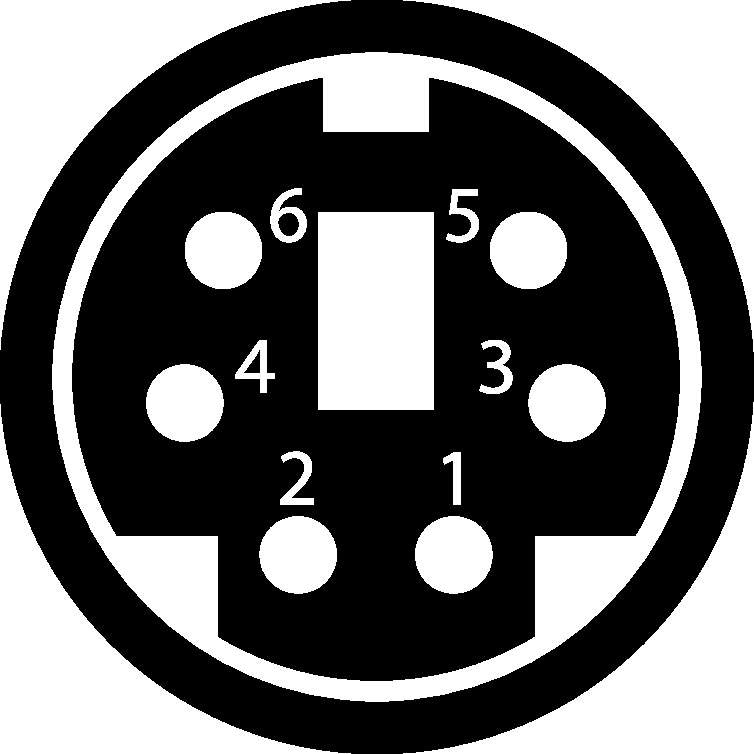
\includegraphics[width=2cm]{figs/MiniDIN-6_Socket_Pinout.pdf}
  \vspace{1em}\par

  \zebra
  \begin{tabular}{clll}
    Pin & Keyboard Port & Mouse Port & Keyboard/Mouse Port \\
    \hline
    1 & Keyboard Data & Mouse Data    & Keyboard Data \\
    2 & Not Connected & Not Connected & Mouse Data \\
    3 & Ground        & Ground        & Ground \\
    4 & +5V DC, 275~mA & +5V DC, 275~mA & +5V DC, 550~mA \\
    5 & Keyboard Clock & Mouse Clock    & Keyboard Clock \\
    6 & Not Connected & Not Connected & Mouse Clock \\
    \hline
  \end{tabular}
  \caption[PS/2 Connector Pin-Out]{\label{fig:kbd-ps2-pinout}PS/2 Connector
    pin-out. This is a view of the PS/2 socket (female connector on mainboards)
    from the front.}
\end{figure*}

\subsection{Communications Protocol}

Both keyboards and mice use the same protocol to exchange data with the
host. Host-to-device and device-to-host directions differ in a number of ways.

\subsubsection{Receiving from the Device}

A timing diagram of a single byte recepction from a device is shown
in~\fcf{fig:kbd-kbd-to-host}. The device only transmits bytes if the clock line
has been consistently high for at least 50~μs. If the clock line is low, the
host is inhibiting reception of new data. Keyboards typically buffer 16 bytes
of data in this case. Mice usually discard data packets.

If the device is clear to transmit, it signals the beginning with the falling
edge of the clock line, and strobes the clock line a total of eleven times:

\begin{description}
\li{Clock 1}: the data line is driven low by the receiver to signal the
beginning of the transmission. This works as a serial start bit.  \li{Clocks
  2–9}: eight data bits are transmitted, least significant bit first.
\li{Clock 10}: an odd parity bit. This bit is clear (\bin{0}) if the number of
set bits in clocks 2–9 (the transmitted byte) is odd. Otherwise, it is set.
\li{Clock 11}: a stop bit, which is always \bin{1}.
\end{description}

The host may stop the device from transmitting at any time by driving the clock
line down for at least 100~μs. Packets may still be transmitted until this
condition is met. If the condition is met during a packet transmission, the
device aborts it, and will restart the entire transmission once the clock line
is released by the host. If this is part of a multi-byte sequence, it will be
restarted from its first byte.

\begin{figure*}
\centering
\begin{tikztimingtable}
  Clock           & 5H 11{CL CH} 5H \\
  Data            & 4H 4L 4D{D0} 4D{D1} 4D{D2} 4D{D3} 4D{D4} 4D{D5} 4D{D6} 4D{D7} 4D{P} 10H \\
\end{tikztimingtable}
\caption[Keyboard/Mouse to Host Communication]{\label{fig:kbd-kbd-to-host}
  Timing of Device (keyboard or mouse) to Host communication. Every byte sent
  includes a start bit (always low), eight bits of data (least significant bit
  first), an odd parity bit, and a stop bit (always high). Eleven clock pulses
  are sent in all. The host clocks data in on the falling edge of the clock
  signal.}
\end{figure*}



\subsubsection{Transmitting to the Device}

A timing diagram of a single byte recepction from the host to a device is shown
in~\fcf{fig:kbd-host-to-kbd}. A host-to-device packet consists of 12 bits. Data
is set while the clock line is low and is read by the device while the clock
is high. The bits sent are as follows:

\begin{description}
\li{Clock 1}: a start bit, always \bin{0}.
\li{Clocks 2–9}: eight data bits are transmitted, least significant bit first.
\li{Clock 10}: an odd parity bit. This bit is clear (\bin{0}) if the number of
set bits in clocks 2–9 (the transmitted byte) is odd. Otherwise, it is set.
\li{Clock 11}: a stop bit, which is always \bin{1}.
\li{Clock 12}: an acknowledge bit, {\em transmitted by the device to the host}.
\end{description}

To transmit a byte to the device, the following sequence of actions must be
performed:

\begin{enumerate}
\item Drive the clock line low for at least 100~μs. This inhibits data
transmission from the device.
\item Drive the data line low. This is the start bit of the transmission.
\item Release the clock line. This signals the device that a host transmission
  is taking place. 
\item Wait for the device to drive the clock line low.
\item Set the data line to the first bit of the byte to send.
\item Wait for the device to release the clock line.
\item Repeat the last three steps to send each bit of the byte and the parity bit.
\item Release the data line.
\item Wait for the device to drive data low.
\item Wait for the device to drive clock low. This is the acknowledge bit from the device.
\item Wait for the device to release the clock and data lines.
\end{enumerate}

There are two timeouts to protect against broken transmissions: the time
between the host driving the clock low for the first time and the device first
driving the clock low should be no greater than 15~ms, and the time between the
device first driving the clock low and the end of the transmission of the stop
bit should be no more than 2~ms. If either of these timeouts occurs, the host
should abort the transmission with an error.

If the command sent to the device requires a response, the response should
arrive within 20~ms, or the host may abort the transaction and generate an
error.

\begin{figure*}
\centering
\begin{tikztimingtable}
  Host Clock           & 2Z 4L 50Z \\
  Host Data            & 4Z 4L 4D{D0} 4D{D1} 4D{D2} 4D{D3} 4D{D4} 4D{D5} 4D{D6} 4D{D7} 4D{P} 4H 8Z \\
  Device Clock           & 7Z LL CH 9{CL CH} CL 7Z \\
  Device Data            & 46Z 4L 6Z \\
\end{tikztimingtable}
\caption[Host to Keyboard/Mouse Communication]{\label{fig:kbd-host-to-kbd}
  Timing of Host to Device (keyboard or mouse) communication. The host
  initiates the transmission, and the device drives the clock signal. Every
  byte sent includes a start bit (always low), eight bits of data (least
  significant bit first), an odd parity bit, a stop bit (always high), and a
  low acknowledge bit (from the keyboard to the host). Twelve clock pulses are
  sent in total. The host writes data when the clock is low and the device
  clocks data in on the rising edge of the clock signal.}
\end{figure*}


\subsection{Keyboard Data Protocol}

Keyboards send data packets on two events: key presses and key
releases. Typematic (auto-repeat) events are sent as multiple press events
followed by a single release event. Each key is identified by its keyboard
matrix scan code, commonly known as simply a scancode. The original IBM PS/2
standard specified three supported sets of scancodes:

\begin{description}
\li{Set 1}: the original IBM PC/XT set of scancodes. Since the original IBM PC
keyboard only had 84 keys, a number of keys on a PS/2 keyboard are not
encoded. Many modern keyboards do not support this set.

\li{Set 2}: this is the default boot-time set of all modern keyboards
attached to the PS/2 port. Scancodes are numbered in a much less rational
way than PC/XT scancodes, but this set is globally supported.

\li{Set 3}: this is the original PS/2 scancode set, which simplifies both
scancodes and the requirements on host-side state machines. Unfortunately, like
set 1, not all keyboards support this scancode set.
\end{description}

Due to its global availability, set 2 is discussed here, and this is the set
the CFT ROM uses.

Set 2 scancodes are variable-width. They come in two varieties: one-byte and
two-byte ones. For two-byte scancodes, the first byte received is {\em
  always\/} \hex{E0}. This value is {\em only\/} encountered for this purpose,
which makes state machines self-synchronising.\footnote{This scheme originates
  in the original Set 1 and is used as a form of aliasing. Naïve software would
  ignore \hex{E0} and operate on the second byte. For instance, by makin the
  Return key issue scancode \hex{5A} and the numeric keypad issue \hex{E0 5A},
  both keys would be interpreted as Return unless the software is purposefully
  trying to distinguish between them.}

Events are either ‘make’ (key press) or ‘break’ (key release) events. Make
events simply report the scancode of the key pressed. A break event is denoted
by the keyboard sending the byte \hex{F0} before the last byte of the
scancode. For single-byte scancodes, this sequence is simply \hex{F0 xx}. For
double scancodes, the sequence is counter-intuitively \hex{E0 F0 xx}. Like
\hex{E0}, \hex{F0} is never used by the keyboard for any purpose other than
break codes.

There are two notable exceptions to the key handling:

\begin{itemize}
\item The ‘Print Screen’ (often marked ‘PrtSc’) key sends {\em two\/}
  keystrokes when pressed, and the keyboard emits the make sequence \hex{E0 12
    E0 7C}. The break sequence is, as expected, \hex{E0 F0 12 E0 F0 7C}. The
  scancode \hex{7C} is the scancode of the numeric keypad multiply (\textsf{*})
  key. On the original IBM PC keyboard, the Print Screen function was accessed
  using Shift and that key. The PS/2 keyboard simulates the AT keyboard in this
  respect, which simulates the XT keyboard: pressing the Print Screen key
  issues an shift-\textsf{*} sequence, using \hex{E0} extensions so that code
  aware of this protocol can detect the key, while code unaware of it (notably
  running on IBM PC/XT or compatible machines) can still function.

\item When pressed, the ‘Pause’ key (used with Control to obtain the ‘Break’
  function) emits the sequence \hex{E1 14 77 E1 F0 14 F0 77}, which includes
  the make {\em and break\/} sequences of two keys. As a result, it is not
  possible to detect whether this key is held down or not because no further
  break packet is sent on its release. On computers unaware of PS/2 keyboards,
  this simulates pressing the Control key if the Control key is not pressed.

  If the Control key {\em is\/} pressed, this key issues the Break\footnote{As
    in ‘stop immediately’, not ‘break’ as in key release.} function with
  scancode \hex{7E}. Somewhat ironically, Break has no break code, which is the
  reason for the Pause button immediately simulating a release.
\end{itemize}

A number of other keys on the keyboard behave in a seemingly erratic function
depending on what modifier keys are active. These are means of making Set 2
keyboards compatible with computers older than the IBM PS/2.

A US keyboard and its scancodes is illustrated in~\fcf{fig:kbd-us}. A
UK keyboard is shown in~\fcf{fig:kbd-uk}. Keys that differ in
function, location or scancode from the US layout are highlighted in
red.


\begin{figure}
  \centering
  % -*- latex -*-
\documentclass[class=memoir]{standalone}
% -*- latex -*-
\usepackage{pgf}
\usepackage{tikz}
%\usetikzlibrary{arrows,positioning,automata,shadows,fit,shapes,counters}
\usetikzlibrary{arrows,positioning,automata,shadows,fit,shapes,patterns}
%\usetikzlibrary{external}
%\tikzexternalize[prefix=tikz/]
%\tikzset{external/system call={xelatex \tikzexternalcheckshellescape -halt-on-error -interaction=batchmode -jobname "\image" "\texsource"}}
\usepackage{standalone}

\usepackage{layout}

%\usepackage[tocindentauto]{tocstyle}

%\usepackage[cam,a4,center]{crop}

\hypersetup{
    pdftitle={CFT Minicomputer Programming Guide},
    pdfauthor={Alexios Chouchoulas},
    pdfkeywords={},
    bookmarksnumbered,
    pagebackref=true,
    breaklinks=true,
%    pdfview=FitH,       % Or try pdfstartview={FitV}, This lead to uncorrect bookmarks
    urlcolor=darkblue,
    colorlinks=true,
    citecolor=cftoutline,          %citeref's color
    linkcolor=cftoutline,
        }

\makeindex
\makeglossaries
% -*- latex -*-

\renewcommand\glspostdescription{}

\newcommand\newglossaryabbr[3]{%
  \newglossaryentry{abbr#1}{name=\glslink{#1}{#2}, text={#2}, description={#3}}
  \newacronym[description={\glslink{abbr#1}{#2}}]{#1}{#1}{#2}
}

\newglossaryentry{IBUS}{name=IBUS,
  description={
  Internal Bus: the single, internal 16-bit bus of the CFT processor.
  }}
  
\newglossaryentry{Data Bus}{name=Data Bus, description={ A
    16-bit bus used to move data between the processor and
    peripherals.  }}
  
\newglossaryentry{Address Bus}{name=Address Bus, description={A
    16-bit bus used to select a peripheral nor memory location to
    access.}}
  
\newglossaryentry{Video Display Unit}{name=Video Display Unit,
  description={ Video Display Unit (VDU): a device that drives a
    display monitor to show character or graphics data on a
    screen. Often also contains one or more input devices (keyboard,
    mouse).}}
  
\newglossaryentry{von Neumann architecture}{name=Von Neumann architecture,
  description={ Named after the work of
    John von Neumann, the von Neumann architecture is a ‘modern’
    computer architecture that includes a register file, arithmetic
    and logic units, memory and input/output, and uses the same
    storage for programs and data.}}

\newglossaryentry{stored program computer}{name=Stored program computer,
  description={ A type of computer that
    uses the same storage for programs and data. All modern computers
    are stored program computers, allowing self-modification of their
    programs. Early designs and many modern microcontrollers stored
    programs and data in separate media, and did not or could not
    treat programs as data.}}

\newglossaryabbr{ALU}{Arithmetic/Logic Unit}{Describe this!}
\newglossaryabbr{ISR}{Interrupt Service Routine}{Describe this!}
\newglossaryentry{UART}{name=UART, description={
    Short for Universal Asynchronous Receiver/Transmitter. UARTs are
    devices that handle asynchronous serial communications such as RS-232, RS-485 or USB.
    }
}
%% \newglossaryentry{alu}{name=\glslink{ALU}{Arithmetic/Logic Unit}, text=Arithmetic/Logic Unit,
%%   description={TODO}}
%% \newacronym[description={\glslink{alu}{Arithmetic/Logic Unit}}]{ALU}{ALU}{Arithmetic/Logic Unit}

\newacronym{SBU}{SBU}{Skip/Branch Unit}

\newacronym{AGL}{AGL}{Address Generation Logic}

\newglossaryentry{DEB}{name=DEB, description={
    Designation of the CFT Debugging/Testing board, a peripheral that
    allows remote control and testing of the computer and its
    peripherals in the style of a virtual front panel. The DEB board
    is discussed in~\ccf{chap:deb}.
}}

\newglossaryentry{VDU}{name=VDU, description={ Video Display
    Unit. Designation of the CFT graphic card and keyboard
    controller. The VDU board is discussed in~\ccf{chap:vdu}.  }}

\newglossaryentry{MSB}{name=MSB, description={
    Most Significant Bits. Usually used to refer to the upper eight bits of a CFT word.
}}
\newglossaryentry{LSB}{name=LSB, description={
    Least Significant Bits. Usually used to refer to the lower eight bits of a CFT word.
}}

\newglossaryentry{NYBBLE}{name=Nybble, description={Sometimes
    nibble. A four-bit quantity, represented as a single hexadecimal
    digit.
}}

% \newacronym{MCU}{MCU}{Micro-Controller Unit}

\newglossaryabbr{MCU}{Micro-Controller Unit}{A single-chip device
  containing a simple microprocessor, general purpose input/output,
  serial input/output, timers, and other useful devices.}

\newacronym{USB}{USB}{Universal Serial Bus}

\newacronym{GPIO}{GPIO}{General-Purpose Input/Output}

\newglossaryentry{Verilog}{name=Verilog,
  description={
    One of the two major hardware
    description languages, the other being VHDL. In the CFT project,
    Verilog is used to perform 74xxx chip-level simulation and
    verification of the CFT processor.
}}

\newglossaryentry{I2C}{name=I²C, description={A two-wire, open-drain
    bus, often used for communication between \gls{MCU}s and
    peripheral chips, including EEPROMs and sensors. For more
    information, please consult
    \url{http://en.wikipedia.org/wiki/I2C}.}}

\newglossaryentry{data stack}{name=Data Stack,
  description=To Do}

\newglossaryentry{postfix}{name=postfix,
  description=To Do}

\newglossaryentry{stack effect comment}{name=stack effect comment,
  description=To Do}

\newglossaryentry{Wait State}{name=Wait State, 
  description={An additional state added to the processor state machine
  to accommodate slow devices. External devices signal their need for a
  wait state to the processor using an appropriate procotol. The
  processor then enters the Wait State and does not leave until the
  device is ready. The processor performs no action during this time,
  hence the name.}}


\newglossaryentry{Twos Complement}{name=Two's Complement,
  description={Currently the most popular means of representing signed
    integers in binary. For a bit width $n$, non-negative numbers $0 \leq
    x < 2^{n-1}$ are represented as unsigned $n$-bit binary
    integers. Negative numbers $-2^{n-1} \leq x < 0$ are represented in
    the form $2^n - x$, with the most significant bit set. On the CFT,
    with $n=16$, this provides a signed range of $[-32,768,
      32,767]$. Two's complement has many useful mathematical
    properties: only one representation of zero, the most significant
    bit also acts as a sign bit, and both addition and subtraction can
    be performed by the same circuitry. For a full discussion, please refer
    to \url{http://en.wikipedia.org/wiki/Two's\_complement}.  }}

\newglossaryentry{Assembly}{name=Assembly, description={A symbolic form of
    \gls{machine code}, meant to be used by humans. Some architectures,
    including the CFT, have simple machine code that can be learned in minutes,
    but the human brain deals better with symbols. Assembly languages also
    provide productivity enhancing features like comments, labels, macros,
    simple arithmetic for literals, and other such facilities. The CFT
    Assembler provides all of these facilities.  }}

\newglossaryentry{DIP}{name=DIP, description={Dual In-line Package, the
    most common integrated circuit package until the introduction of
    Surface Mount Technology: DIP chips have two rows of pins, with pins
    set at distances of 2.54~mm (0.1~inch).
}}

\newglossaryentry{PLCC}{name=PLCC, description={Plastic Leaded Chip
    Carrier, a square surface mount chip packaging easily adapted to
    2.54mm grids by means of suitable IC sockets. The CFT uses
    numerous PLCC chips to save board space and because they offer
    more choice of chips, and thus better value for money. All CFT
    PLCC packages are either Flash devices or UARTs.}}

\newglossaryentry{MEM}{name=MEM, description={ Designation of the
    memory board, which, depending on construction details provides up
    to 512 or 1,024 kWords of RAM and/or ROM. The MEM board is
    discussed in~\ccf{chap:mem}.
}}

\newglossaryentry{MBU}{name=MBU, description={Designation of the
    Memory Banking Unit. This was originally slated to be a separate
    peripheral, but has become so important to the project that it is
    now considered to be part of the processor, and constructed as
    such. The MBU breaks memory space in logical and physical
    addresses, and allows the processor's limited 64 kWord address
    space to be expanded to a 21 bit, 2,048 kWord address space using
    memory banking techniques. More details may be found in
    \ccf{chap:mbu}.  }}

\newglossaryentry{Interrupt Service Routine}{name=Interrupt Service Routine (ISR),
  description={TO DO}}

\newglossaryentry{Page}{name=Page, description={The CFT instruction set allows
    for a 10-bit operand, which allows instructions to address up to
    $2^{10}=1024$ locations. This 1,024-word range is known as a page. The CFT
    address space contains 64 such 1 kWord pages. \gls{Page Zero} at addresses
    \hex{0000}–\hex{03FF} has special significance in the programming model, as
    discussed in~\cf{sec:memory-space}.
 }}

\newglossaryentry{Page Zero}{name=Page Zero, description={Page Zero occupies
    the first 1,024 addresses (\hex{0000}–\hex{03FFF}) of the memory address
    space. It is used to simulate 1,024 registers, global variables or
    constants accessible from anywhere in memory. Addresses
    \hex{0080}–\hex{00FF} are autoindex locations: they increment when accessed
    in \gls{Indirect Mode}.}}

\newglossaryentry{Addressing Mode}{name=Addressing Mode, description={An
    addressing mode is the method in which an instruction operand is
    interpreted. The CFT can treat operands as literal values (\gls{Literal
      Mode}), addresses of data (\gls{Direct Mode}), or addresses of addresses
    of data (\gls{Indirect Mode}), similar to pointersin high-level languages
    such as C and Pascal. Addressing modes are discussed
    in~\cf{sec:addressing-modes}}.}

\newglossaryentry{Indirect Mode}{name=Indirect Mode, description={An addressing
    mode where an instruction operand identifies the memory location which
    contains the address of the data to access. Compare \gls{Direct
      Mode}. Addressing modes are discussed in~\cf{sec:addressing-modes}.}}

\newglossaryentry{Direct Mode}{name=Direct Mode, description={An addressing
    mode where an instruction operand identifies the memory location of the
    data to access. Compare \gls{Indirect Mode}. Addressing modes are discussed
    in~\cf{sec:addressing-modes}.}}

\newglossaryentry{Literal Mode}{name=Literal Mode, description={An addressing
    mode where an instruction operand identifies the memory location of the
    data to access. Compare \gls{Indirect Mode}. Addressing modes are discussed
    in~\cf{sec:addressing-modes}.}}

\newglossaryentry{register}{name=Register, description={ A data storage device
    inside a processor. Registers are usually faster than memory, and so are
    used to store intermediate results. In many architectures, notably
    \glspl{ABA}, the only way for the processor to
    manipulate data is to transfer it to a register, operate on the register,
    then transfer it back to its intended location. CFT registers are discussed
    in~\cf{sec:registers}.}}

\newglossaryentry{Accumulator}{name=Accumulator, description={The main
    \gls{register} in an \gls{ABA}. Data must be transferred to the Accumulator
    before it can be operated on by the processor. In the CFT, the Accumulator
    is the only such general purpose register available. The term comes from
    the days of tabulating machines, which used accumulators to accumulate
    (sum) numbers. The Accumulator is designated ‘\AC’ on the CFT. Its hardware
    design is discussed in~\cf{sec:major-registers} and its operation from a
    programmer's point of view is discussed in~\cf{sec:accumulator}.}}

\newglossaryabbr{ABA}{Accumulator-Based Architecture}{A processor architecture
  built around a single (or in some cases, a few) accumulators. Most early
  computers followed this design because of its simplicity, and the CFT does
  too. Having a single register draastically simplifies the instruction format,
  too: from a two-operand instruction format (source, destination), we move to
  a single operand (source or destination). The other operand is always the
  accumulator.  }

\newglossaryentry{nybble}{name=Nybble, description={(sometimes nibble)
    A 4-bit quantity, corresponding to one hexadecimal digit, half a
    byte, or one quarter of a CFT \gls{Word}.}}

\newglossaryentry{Word}{name=Word, description={One CFT Word is a
    16-bit quantity. CFT memory and I/O accesses transfer exactly one
    word each. CFT instructions are also one Word wide. This is not to
    be confused with the Forth concept of a \gls{word} (an identifier).}}

\newglossaryentry{word}{name=Word, description={A Forth word is any
    sequence of non-whitespace characters that is not a number. This
    is not to be confused with the more common concept of the
    \gls{Word} as a numeric datatype.}}

\newglossaryentry{machine code}{name=Machine code, description={Machine code is
    the native language of every processor, where machine instructions and data
    are represented in binary. Machine code is easy for the computer to
    process, but humans find it useful to apply abstraction layers to it: data
    are represented in other bases (octal, decimal and hexadecimal being the
    most common), and symbolic instruction names (rather than binary
    instruction numbers) are used. This set of abstractions is \gls{Assembly}
    language.}}

\newglossaryentry{disk label}{name=Disk Label, description={ A disk label
    stores information about a storage device (not always a disk), including a
    magic number to help detect the block, some optional boot code, and
    definitions for one to sixteen \glspl{disk slice} (partitions). The disk
    label always resides in the first block of a device. The best-known disk
    label format is the MS-DOS Master Boot Record, MBR. The CFT's disk label is
    discussed in~\cf{sec:disk-label}.}}

\newglossaryentry{disk slice}{name=Disk Slice, description={Part of a disk intended to
    hold a \gls{filesystem} or other data. Disks are sliced to make them easier
    to manage, so different operating systems can be used, to control the size
    of stored data, and to avoid corruption in one filesystem destroying all
    data. In the MS-DOS world, slices are known as ‘partitions’, and the
    \gls{disk label} is known as a ‘partition table’ or ‘Master Boot Record’
    depending whether it resides on a data disk or bootable disk. The CFT's
    slice scheme is discussed in~\cf{sec:disk-slices}}.}

\newglossaryentry{filesystem}{name=Filesystem, description={ A large data
    structure used to view a storage medium as a hierarchical collection of
    data objects called files. The filesystem abstracts the natural
    array-of-blocks structure of the storage medium, and provides the user with
    an interface for creating, reading and otherwise operating on files by
    their name, location and other attributes. Files can be larger than the
    natural block size, and this is again handled transparently by the
    filesystem code. The CFT's filesystem is described in~\cf{sec:fs}}}

\newglossaryabbr{VD}{Volume Directory}{A data structure
  describing a CFT \gls{filesystem}. Comparable to a Unix filesystem
  superblock. The VDD is the exact same data structure as a
  \gls{DD}. The difference is in the magic number and the contents of
  the first directory slot (the header), which contains a volume
  header structure.}

\newglossaryabbr{DD}{Directory Descriptor}{A data structure describing
  a directory in a CFT \gls{filesystem}.}

\newglossaryentry{block pointer}{name=Block Pointer, description={A
    32-bit value (\gls{MSB} first) denoting the number of a filesystem
    block. A filesystem's first block is block \hex{00000000}.}}

\newglossaryabbr{DH}{Directory Header}{A data structure describing a
  CFT directory. This is the first entry of a \gls{DD}.}

\newglossaryabbr{OOP}{Object Oriented Programming}{A programming
  paradigm where data and code are bundled together in data structures
  called objects. Programs are built based on the interactions and
  interrelations of these objects.}

\newglossaryentry{descriptor}{name=Descriptor, description={In the CFT Filesystem, a data structure
    that holds metadata on an object in the CFT filesystem. Descriptors share
    some common metadata (e.g. filenames, flags, creation time and date). They
    are located inside container objects (volumes and directories). Containers
    and descriptors are discussed in~\cfp{sec:fs-containers}.}}

\newglossaryentry{volume}{name=Volume, description={A \gls{disk slice} which
    has been structured according to the CFT Filesystem. In \gls{OOP} terms, a
    volume is the object (instance) and the CFT Filesystem is the class.}}

\newglossaryentry{container}{name=Container, description={In the CFT
    Filesystem, a data structure that contains other filesystem objects. Entire
    filesystem \glspl{volume} are containers, and so are directories. Each
    container owns a maximum number of \glspl{descriptor}, identifying the
    contained objects. Once this limit is reached, continuation blocks are
    allocated for the container. These continuation blocks form a doubly linked
    list. Containers are discussed in~\fcf{sec:fs-containers}.}}

\newglossaryabbr{PEL}{Picture Element}{The smallest addressable
  picture element of a display mode. A PEL is usually a block of
  multiple pixels.}

\newglossaryabbr{MTBF}{Mean Time Between Failures}{The average life
  expectancy of a device.}

\newglossaryentry{codepoint}{name=Codepoint, description={A number
    identifying a character within a character set. For example, in
    the ASCII set, codepoint 65 is the character ‘A’.}}

\newglossaryabbr{SDRAM}{Synchronous Dynamic Random Access Memory}{A
  type of modern dynamic RAM that operates using a clock, not
  asynchronously like original DRAMs. The memory contains a command
  pipeline, because data appears on the bus two to three clock ticks
  after a read is signalled. Multiple reads are pipelined, making the
  memory very fast for many use patterns.}

\newglossaryabbr{SRAM}{Static Random Access Memory}{A type of
  relatively low-density memory that trades off capacity and price for
  speed and interface simplicity. SRAMs do not need to be refreshed
  and are faster than similar dynamic RAMs.}

\newglossaryentry{extended instruction}{name=Instruction!Extended,
  description={An address in I/O space that provides side effects
    useful enough to be seen as extending the processor's instruction
    set. They are usually aliases of single \asm{IN}, \asm{OUT} or
    \asm{IOT} instructions.}}

\newglossaryabbr{SR}{Switch Register}{A 16-bit read-only register that
  provides the value of the 16 data entry switches on the front
  panel.}

\newglossaryabbr{DSR}{DIP Switch Register}{A 12 to 16-bit read-only
  register driven by a bank of DIP switches on the Front Panel
  Controller board. The DSR can be used to set non-volatile prefrences
  for the computer's early boot.}

\newglossaryabbr{MFD}{Multi-Function Display}{A bank of 16 lights on
  the front panel which can display a user-selectable register. The
  user can elect to show the value of the Data Register, Output
  Register, or the 15-bit microcode store address. A switch on the
  front panel is used to do this.}


\usepackage{listings}
\lstset{%
  xleftmargin=35pt,
  xrightmargin=5pt,
  basicstyle={\ttfamily},
  backgroundcolor=\color{cfthl!25},
  rulecolor=\color{cfthl!25},
  framesep=5pt,
  rulesep=5pt,
  frame=tlrb,
  framexleftmargin=10pt,
  flexiblecolumns=true,
  keepspaces=true,
  numbers=left,
  numbersep=5pt,
  numberstyle={\scriptsize\sffamily\color{cftlight}}
}




%%%%%%%%%%%%%%%%%%%%%%%%%%%%%%%%%%%%%%%%%%%%%%%%%%%%%%%%%%%%%%%%%%%%%%%%%%%%%%%
%%
%% LISTS OF THINGS
%%
%%%%%%%%%%%%%%%%%%%%%%%%%%%%%%%%%%%%%%%%%%%%%%%%%%%%%%%%%%%%%%%%%%%%%%%%%%%%%%%

%% %%%\addtolength\cftfignumwidth{1.5em}
\makeatletter
%% \addtolength{\cftchapternumwidth}{0.5em}
%% \addtolength{\cftsectionnumwidth}{0.5em}
%% \addtolength{\cftsubsectionnumwidth}{0.5em}
%% \addtolength{\cftfigurenumwidth}{0.5em}
%% \addtolength{\cfttablenumwidth}{0.5em}
\renewcommand*\l@section{\@dottedtocline{1}{1.5em}{2.3em}}
\renewcommand*\l@subsection{\@dottedtocline{2}{3.8em}{3.2em}}
\renewcommand*\l@subsubsection{\@dottedtocline{3}{7.0em}{4.1em}}
\renewcommand*\l@paragraph{\@dottedtocline{4}{10em}{5em}}
\renewcommand*\l@subparagraph{\@dottedtocline{5}{12em}{6em}}
\setcounter{maxsecnumdepth}{3}

%\addtolength{\cftschematicsnumwidth}{1em}
\renewcommand{\@pnumwidth}{3em}
\renewcommand{\@tocrmarg}{4em}
\makeatother

%\newcommand\listalgname{List of Algorithms} 
%\newlistof{alg}{algorithm}

%
% Schematics
%

\newcommand\listschematicname{List of Schematics} 
\newlistof{listofschematic}{los}{\listschematicname}
\newcounter{schematic}
\newcommand{\schematic}[1]{%
  \refstepcounter{schematic}%
  \par\noindent\textbf{Schematic \theschematic. #1}
  \addcontentsline{los}{section}{\protect\numberline{\theschematic}#1}\par%
}
\newcommand\listofschematics\listofschematic

%
% I/O Ports
%

\newcommand\listioportname{List of Input/Output Ports} 
\newlistof{listofioport}{loioport}{\listioportname}
%% \newcommand{\registerioport}[1]{%
%%   \refstepcounter{ioport}%
%%   \addcontentsline{loioport}{section}{\protect\numberline{\ }%
%% }
\newcommand\listofioports\listofioport



\newcommand\caution[1]{\textcolor{caution}{\textbf{#1}}}
%\newcommand\todo[1]{\textcolor{caution}{\bf{TODO: #1}}}

%
% Tasks
%

\newcommand\listtasksname{List of Incomplete Tasks} 
\newlistof{listoftask}{lotasks}{\listtasksname}
\newcounter{task}
\newcommand{\todo}[1]{%
  \refstepcounter{task}%
  {\textcolor{caution}{\textbf{TODO: #1}}}
  \addcontentsline{lotasks}{section}{\protect\numberline{\arabic{task}}To Do: #1}\par%
}
\newcommand{\bug}[2]{%
  \refstepcounter{task}%
  {\textcolor{caution}{\textbf{BUG: #1 #2}}}
  \addcontentsline{lotasks}{section}{\protect\numberline{\arabic{task}}Bug: #1}\par%
}
\newcommand\listoftasks\listoftask

%
% Data structures
%

\newcommand\listdatastructurename{List of Data Structures} 
\newlistof{listofdatastructure}{lods}{\listdatastructurename}
\newcounter{datastructure}
%\newcommand{\datastructure}[1]{%
%  \refstepcounter{datastructure}%
%  \par\noindent\textbf{Data Structure \thedatastructure. #1}
%  \addcontentsline{lods}{section}{\protect\numberline{\thedatastructure}#1}\par%
%}
\newcommand\listofdatastructures\listofdatastructure



%%%%%%%%%%%%%%%%%%%%%%%%%%%%%%%%%%%%%%%%%%%%%%%%%%%%%%%%%%%%%%%%%%%%%%%%%%%%%%%
%%
%% SECTION STYLING
%%
%%%%%%%%%%%%%%%%%%%%%%%%%%%%%%%%%%%%%%%%%%%%%%%%%%%%%%%%%%%%%%%%%%%%%%%%%%%%%%%



%% \usepackage{kpfonts}
\usepackage[explicit]{titlesec}

\counterwithin*{chapter}{part}
\counterwithin*{figure}{chapter}
\counterwithin*{schematic}{chapter}
\counterwithin*{datastructure}{chapter}
\counterwithin*{table}{chapter}

%%%%%%%%%%%%%%%%%%%%%%%%%%%%%%%%%%%%%%%%%%%%%%%%%%%%%%%%%%%%%%%%%%%%%%%%%%%%%%%

\renewcommand\thepart{\Alph{part}}
\cftpagenumbersoff{part}
%\newcommand*\partlabel{}

\makeatletter
\patchcmd{\l@part}{\hss#2}{}{}{}
\makeatother


\renewcommand\partnamefont{\normalfont\sffamily\Huge\scshape}
\renewcommand\partnumfont{\bfseries}
\renewcommand\printparttitle[1]{
  \thispagestyle{empty}
    \begin{tikzpicture}[remember picture,overlay]
      \node[yshift=-\paperheight, draw opacity=0] at (current page.north west)
           {\begin{tikzpicture}[remember picture, overlay]
               \draw[fill=cftlight] (0,0) rectangle
               (\paperwidth,\paperheight);
               \draw[fill=cftoutline] (0,1cm) rectangle
               (\paperwidth,0);
               \node[anchor=east,yshift=0.5\paperheight,xshift=.87\paperwidth,rectangle]
                    {\scalebox{2}{\color{white}\printpartname~\printpartnum}};
                    \node[anchor=east,yshift=0.43\paperheight,xshift=.87\paperwidth,rectangle]
                         {\scalebox{1.5}{\color{white} #1}};
             \end{tikzpicture}
           };
    \end{tikzpicture}
}


\newcommand*\chapterlabel{}
\titleformat{\chapter}
  {\gdef\chapterlabel{}
   \normalfont\sffamily\Huge}
  {\gdef\chapterlabel{\thechapter\ }}{0pt}
  {%
    \setcounter{page}{1}
    \begin{tikzpicture}[remember picture,overlay]
    \node[yshift=-5cm, draw opacity=0] at (current page.north west)
      {\begin{tikzpicture}[remember picture, overlay]
        \draw[fill=cftlight] (0,0) rectangle
          (\paperwidth,5cm);
        \draw[fill=cftoutline] (0,0.25cm) rectangle
          (\paperwidth,0);
        \node[anchor=east,yshift=2cm,xshift=.87\paperwidth,rectangle]
              {\color{white}\chapterlabel#1};
       \end{tikzpicture}
      };
   \end{tikzpicture}
  }
\titlespacing*{\chapter}{0pt}{50pt}{20pt}

\titleformat{\section}
            {\gdef\sectionlabel{}\normalfont\sffamily\Large}
            {\gdef\sectionlabel{\thesection\ }}{0pt}
            {\color{cftoutline}\thesection\quad #1\\
              \titlerule[2pt]
            }[{\vspace{-30pt}\color{cftoutline}\rule{\textwidth}{2pt}}]


\titleformat{\subsection}
  {\gdef\subsectionlabel{}
   \normalfont\sffamily\bfseries\large}
  {\gdef\subsectionlabel{\thesubsection\ }}{0pt}
  {\color{cftoutline}\thesubsection\quad #1}


\titleformat{\subsubsection}
  {\gdef\subsubsectionlabel{}
   \normalfont\sffamily\large}
  {\gdef\subsubsectionlabel{\thesubsubsection\ }}{0pt}
  {\color{cftoutline}#1}


%%%%%%%%%%%%%%%%%%%%%%%%%%%%%%%%%%%%%%%%%%%%%%%%%%%%%%%%%%%%%%%%%%%%%%%%%%%%%%%










%% \titleformat{\paragraph}
%%   {\gdef\chapterlabel{}
%%    \normalfont\bfseries}
%%   {\gdef\chapterlabel{\theparagraph\ }}{0pt}
%%   {\color{cftoutline}#1}



%\geometry{a4paper, hoffset=0in, voffset=-.25in, left=1.5cm, right=1.5cm,
%  top=2.5cm, bottom=2.5cm}
%\geometry{paperwidth=17.5cm, paperheight=23.1cm, hoffset=0in, voffset=-.25in, left=1in, right=1in,
%  top=1in, bottom=1in}
\geometry{a4paper, hoffset=0in, left=1.2in, right=1.2in,
  top=1.2in, bottom=1.2in, includefoot, footskip=40pt}
%\sloppy


% Fonts
%\defaultfontfeatures{Mapping=tex-text}
\setmainfont{Minion Pro}
\setsansfont{Myriad Pro}
\setmonofont[]{Inconsolata}


% Not really used here, but never mind.
\setlength\columnsep{7mm}


% Input our local macro definitions
% -*- latex -*-

\definecolor{caution}{RGB}{192,0,0}

\newcommand\textcond{\fontspec{Myriad Pro Condensed}}

% Primary index entries
\newcommand\pie[1]{\textbf{\hyperpage{#1}}}

% Use hyperlinking when rendering PDFs
\newcommand{\barecf}[1]{\hyperref[#1]{\ref*{#1}}}
\newcommand{\cf}[2][section]{\hyperref[#2]{%
        \ifthenelse{\equal{\pageref*{#2}}{\thepage}}%
        {#1 \ref*{#2}}%
        {#1 \ref*{#2} (p.~\pageref*{#2})}%
}}
\newcommand{\cfp}[2][section]{\hyperref[#2]{%
        \ifthenelse{\equal{\pageref*{#2}}{\thepage}}%
        {#1 \ref*{#2}}%
        {#1 \ref*{#2}, p.~\pageref*{#2}}%
}}
\newcommand{\fcf}[1]{\cf[figure]{#1}}
\newcommand{\fcfp}[1]{\cfp[figure]{#1}}
\newcommand{\tcf}[1]{\cf[table]{#1}}
\newcommand{\tcfp}[1]{\cfp[table]{#1}}
\newcommand{\ccf}[1]{\cf[chapter]{#1}}
\newcommand{\ccfp}[1]{\cfp[chapter]{#1}}
%
\newcommand{\npcf}[2][section]{\hyperref[#2]{#1 \ref*{#2}}}
\newcommand{\appcf}[1]{\cf[appendix]{#1}}
\newcommand{\ecf}[1]{\cf[equation]{#1}}
\newcommand{\algcf}[1]{\cf[algorithm]{#1}}
\newcommand{\npappcf}[1]{\npcf[appendix]{#1}}
\newcommand{\npccf}[1]{\npcf[chapter]{#1}}
\newcommand{\npfcf}[1]{\npcf[figure]{#1}}
\newcommand{\nptcf}[1]{\npcf[table]{#1}}
\newcommand{\npecf}[1]{\npcf[equation]{#1}}
\newcommand{\npalgcf}[1]{\npcf[algorithm]{#1}}

\newcommand\hyperemail[1]{\sffamily\href{mailto:#1}{#1}}
\newcommand\link[1]{\sffamily\href{http://#1}{#1}}
\newcommand\ahref[2]{\sffamily\href{#1}{#2}}

\newcommand\op[1]{{\ttfamily #1}}
\newcommand\fwni[1]{{\ttfamily{#1}}}
\newcommand\fw[1]{\fwni{#1}\index{#1@\protect\fwni{#1}}}
%                           \index{#1@\fwni{#1}|(pie}%

\newcommand\f[1]{{\texttt{#1}}}
\newcommand\hex[1]{\textsf{#1}}
\newcommand\bin[1]{\textsf{#1}}
\newcommand\bitmap[1]{\texttt{#1}}
\newcommand\bus[1]{{#1}}
\newcommand\unit[1]{{#1}}
\newcommand\IBUS{\bus{\gls{IBUS}\index{IBUS}}}
\newcommand\DBUS{\bus{\gls{Data Bus}\index{Data Bus}}}
\newcommand\ABUS{\bus{\gls{Address Bus}\index{Address Bus}}}
\newcommand\ALU{\unit{\gls{ALU}\index{ALU}}}
\newcommand\SBU{\unit{\gls{SBU}\index{SBU}}}
\newcommand\AGL{\unit{\gls{AGL}\index{AGL}}}
\newcommand\register[1]{\textsf{#1}\index{Registers!#1}}
\newcommand\A{\register{AC}}
\newcommand\AC{\A}
\newcommand\Areg{\A}
\newcommand\Lreg{\register{L}}
\newcommand\Ireg{\register{I}}
\newcommand\Zreg{\register{Z}}
\newcommand\Vreg{\register{V}}
\newcommand\Nreg{\register{N}}
\newcommand\AR{\register{AR}}
\newcommand\MAR{\AR}
\newcommand\DR{\register{DR}}
\newcommand\PC{\register{PC}}
\newcommand\IR{\register{IR}}

\newcommand{\asm}[1]{\texttt{#1}}
\newcommand{\instr}[1]{\asm{#1}}
\newcommand{\nsni}[1]{$\overline{\mbox{\textsf{{#1}}}}$}
\newcommand{\ns}[1]{\nsni{#1}\index{#1@{$\protect\overline{\protect\mbox{\textsf{#1}}}$}}}
\newcommand{\psni}[1]{\textsf{#1}}
\newcommand{\ps}[1]{\psni{#1}\index{#1@\psni{#1}}}
\newcommand{\lt}[1]{\textsf{#1}}
\newcommand{\sw}[1]{\textsf{#1\index{Switch, front panel!#1}}}
\newcommand{\HC}[1]{\chip{74HC{#1}}}
\newcommand{\HCT}[1]{\chip{74HCT{#1}}}
\newcommand{\chip}[1]{#1\index{#1}}

\newcommand{\schpt}[1]{#1\textsf{#1}}
\newcommand{\farnell}[1]{#1}

\newcommand\BUS[2]{\ps{#1}$_{\mbox{\scriptsize #2}}$}
\newcommand\nBUS[2]{\ns{#1}$_{\mbox{\scriptsize #2}}$}

\newcommand\UINSTR{\ns{uINSTR18}}
\newcommand\HALT{\ns{HALT}}
\newcommand\END{\ns{END}}
\newcommand\IRQ{\ns{IRQ}}
\newcommand\IRQS{\ns{IRQS}}
\newcommand\IRQn[1]{\nBUS{IRQ}{#1}}
\newcommand\RUNITn[1]{\BUS{RUNIT}{#1}}
\newcommand\WUNITn[1]{\BUS{WUNIT}{#1}}
\newcommand\TPA{\ps{TPA}}
\newcommand\TPC{\ps{TPC}}
\newcommand\WAC{\ns{WAC}}
\newcommand\WALU{\ns{WALU}}
\newcommand\WDR{\ns{WDR}}
\newcommand\WIR{\ns{WIR}}
\newcommand\WMAR{\ns{WMAR}}
\newcommand\WPC{\ns{WPC}}
\newcommand\SYSDEV{\ns{SYSDEV}}
\newcommand\IODEV[1]{\ns{IODEV{#1}XX}}
\newcommand\OPIFn[1]{\BUS{OPIF}{#1}}
\newcommand\OPIF{\ps{OPIF}}
\newcommand\GUARDPULSE{\ns{GUARD}}
\newcommand\GP{\GUARDPULSE}
\newcommand\CLOCK[1]{\BUS{CLK}{#1}}
\newcommand\RSTHOLD{\ns{RSTHOLD}}
\newcommand\BOE{\ns{BOE}}
\newcommand\UOE{\ns{UOE}}
\newcommand\SKIP{\ns{SKIP}}
\newcommand\AINDEX{\ps{AINDEX}}
\newcommand\CLL{\ns{CLL}}
\newcommand\CPL{\ns{CPL}}
\newcommand\CLI{\ns{CLI}}
\newcommand\STI{\ns{STI}}
\newcommand\IRn[1]{\BUS{IR}{#1}}
\newcommand\PCn[1]{\BUS{PC}{#1}}
\newcommand\IBUSn[1]{\BUS{IBUS}{#1}}
\newcommand\DBUSn[1]{\BUS{DBUS}{#1}}
\newcommand\ABUSn[1]{\BUS{AB}{#1}}
\newcommand\AEXTn[1]{\BUS{AEXT}{#1}}
\newcommand\ISROLL{\ps{ISROLL}}
\newcommand\RAC{\ns{RAC}}
\newcommand\RAGL{\ns{RAGL}}
\newcommand\RDR{\ns{RDR}}
\newcommand\RPC{\ns{RPC}}
\newcommand\INCPC{\ns{INCPC}}
\newcommand\STPAC{\ns{STPAC}}
\newcommand\STPDR{\ns{STPDR}}
\newcommand\INCAC{\STPAC}
\newcommand\INCDR{\STPDR}
\newcommand\DEC{\ns{DEC}}
\newcommand\MEM{\ns{MEM}}
\newcommand\IO{\ns{IO}}
\newcommand\R{\ns{R}}
\newcommand\WRITE{\ns{W}}
\newcommand\WEN{\ns{WEN}}
\newcommand\READ{\ns{R}}
\newcommand\FL{\ps{FL}}
\newcommand\FV{\ps{FV}}
\newcommand\FZERO{\ps{FZERO}}
\newcommand\FNEG{\ps{FNEG}}
\newcommand\RESET{\ns{RESET}}
\newcommand\abbr[1]{#1}
\newcommand\SKIPEXT{\ns{SKIPEXT}}
\newcommand\ENDEXT{\ns{ENDEXT}}
\newcommand\WS{\ns{WS}}
\newcommand\UPC{\ps{µPC}}
\newcommand\UCB{\ps{µCB}}

\newcommand\NB{\textbf{Nota Bene:\ }}

\newcommand\bit[1]{{\texttt{#1}}}

\newcommand\notes[1]{{\small\verbatiminput{#1}}}

\newcommand\field[1]{\textsf{#1}}
\newcommand\port[1]{\textsf{#1}}

\newcommand\cftin[1]{\textsf{#1}}
\newcommand\cftout[1]{\textsf{#1}}
\let\cftcode\cftout
\let\cftkbd\cftin

\newcommand\li[1]{\item{\bfseries #1}}

% Temporary question environment
\newcommand\question[2]{\textbf{#1} #2}


%%%%%%%%%%%%%%%%%%%%%%%%%%%%%%%%%%%%%%%%%%%%%%%%%%%%%%%%%%%%%%%%%%%%%%%%%%%%%%%
%
% THE I/O PORT AND EXTENDED COMMAND INDEX
%
%%%%%%%%%%%%%%%%%%%%%%%%%%%%%%%%%%%%%%%%%%%%%%%%%%%%%%%%%%%%%%%%%%%%%%%%%%%%%%%

%% \makeatletter
%% \newcommand\ioport@[4]{%
%%   \label{ioport:#1-#4}
%%   \vspace{0.5em}
%%   \noindent\hex{\bfseries{#2}} (\texttt{#1}): {\bfseries\asm{\bfseries{#3}}} — {#4}
%%   \vspace{0.5em}
%% }
%
%
% \ioport{port}{crwvehf}{regname}{descr}
%
%% \newcommand\ioport[4]{%
%%   \ioport@{#1}{#2}{#3}{#4}
%%   \addcontentsline{loioport}{section}{\hex{#2} (\texttt{#1}) \textbf{\asm{#3}} — soup}%
%% }

% \begin{ioport}{VDU}{1F0}{--wvehf}{MCR0}{Mode Control Register 0}
% ...
% \end{ioport}

\newenvironment{ioport}[5]{%
  \vspace{0.5em}
  \addcontentsline{loioport}{section}{\hex{#2} (\texttt{#3}) \textbf{\cftout{#1} \cftout{#4} — #5}}%
  \noindent\hex{\bfseries{#2}} (\texttt{#3}): {\bfseries\asm{\bfseries{#4}}} — {#5}%
  \noindent%
}{%
  \vspace{0.5em}
}

% \begin{extcmd}{PFP}{SR1}{4409}{009}{--wvehf}{Mode Control Register 0}
% ...
% \end{extcmd}
\newenvironment{extcmd}[7]{%
  \vspace{0.5em}
  \addcontentsline{loioport}{section}{\hex{#2} (\texttt{#4}) \textbf{\cftout{#1} \cftout{#2} — #6}}%
  \noindent\hex{\bfseries{#2}} \hex{#3} (I/O port \hex{#4} — \texttt{#5}): {\bfseries{#6}}%
  \noindent%
}{%
  \vspace{0.5em}
}

%\newcommand\extcmda[7]{%
%  \label{ioport:#5-#2}
%  \vspace{0.5em}
%  \noindent\hex{\bfseries{#2}} (\texttt{#1}): {\bfseries\asm{\bfseries{#3}}} — {#4}
%  \vspace{0.5em}
%  \ioport{#4}{#5}{#1}{#7}
%}
%\newcommand\extcmd[7]{% 
%  \extcmda{#1}{#2}{#3}{#4}{#5}{#6}{#7}
%  \addcontentsline{loioport}{section}{\hex{#5} (\texttt{#4}) \textbf{\asm{#1}} — {#6}}%
%  \addcontentsline{loioport}{section}{\protect\numberline{\ }%
%}
\makeatother


%%%%%%%%%%%%%%%%%%%%%%%%%%%%%%%%%%%%%%%%%%%%%%%%%%%%%%%%%%%%%%%%%%%%%%%%%%%%%%%
%
% CODE FOR DISPLAYING AND INDEXING SCHEMATICS
%
%%%%%%%%%%%%%%%%%%%%%%%%%%%%%%%%%%%%%%%%%%%%%%%%%%%%%%%%%%%%%%%%%%%%%%%%%%%%%%%


% \schematic{page number}{description}{label}
\def\schematicsFile{figs/schematics.pdf}
\newcommand\includesch[3]{%
  \stepcounter{subsection}%
  \phantomsection%
  \addcontentsline{toc}{subsection}{\protect\numberline{\thesubsection} #2}%
  \includeschns{#1}{#2}{#3}
}

\newcommand\includeschns[3]{%
  \label{#3}%
  \stepcounter{schematic}%
  \addcontentsline{los}{section}{\protect\numberline{\theschematic} #2}%
  \includepdf[
    pages={#1}
    ,landscape,
    ,fitpaper=true,
%    ,pagecommand={\thispagestyle{lscape}}  
    ,pagecommand={\thispagestyle{empty}}  
  ]{\schematicsFile}%
}


\newcommand\tU{$\uparrow$}
\newcommand\tD{$\downarrow$}

\newcommand\lstkbd[1]{\mathbf{\textbf{#1}}}
%\newcommand\lstfkbd[1]{\underline{\mathbf{\textbf{#1}}}}
\newcommand\lstfkbd[1]{\color{cftoutline}{\mathbf{\textbf{#1}}}}
\lstset{%
        keywordstyle=\fontspec{Inconsolata Bold},%
        keywordstyle=[2]\color{cftoutline}\fontspec{Inconsolata Bold},%
        keywordstyle=[3]\fontspec{Inconsolata Bold},%
        commentstyle=\color{cftlight}%
}
\lstdefinestyle{deb}{mathescape=true,numbers=none}
\lstdefinestyle{forthprogram}{}
\lstdefinelanguage{cftasm}{%
        mathescape=true,
        morekeywords={TRAP,IOT,LOAD,STORE,IN,OUT,JMP,JSR,ADD,AND,OR,%
                      XOR,OP1,OP2,ISZ,LIA,R,I,IFL,IFV,CLA,CLL,NOT,%
                      INC,CPL,RBL,RBR,RNL,RNR,NOP,SNA,SZA,SSL,SSV,SKIP,%
                      SNN,SNZ,SCL,SCV,CLI,SEI,SEL,NEG,ING,LI,SPA,SNP,RET,%
                      RTT,RTI,SBL,SBR},%
        morekeywords=[2]{.equ,.reg,.include,.word,.fill,%
                      .str,.data,.strp,.strn,.page,.macro,.end},%
        alsoletter=.,%
        sensitive=false,%
        morecomment=[l]{/},%
        morecomment=[l]{;},%
}

\lstdefinestyle{longmcasm}{%
        language=mcasm,
        xleftmargin=25pt,
        xrightmargin=5pt,
        framexleftmargin=20pt,
        basicstyle={\footnotesize\ttfamily},
}
\lstdefinelanguage{mcasm}{%
        mathescape=false,
        morekeywords={cond,field,signal,start,hold},%
        morekeywords=[2]{\#define,\#ifdef,\#endif,\#if,\#undef,\#line,\#warning,\#warn,\#error},%
        morekeywords=[3]{INT,RST,V,L,OP,I,SKIP,INC,uaddr},%
        alsoletter=\#,%
        sensitive=false,%
        morecomment=[l]{//},%
        %morecomment=[s]{( }{ )},%
}


\lstdefinelanguage{forth}{%
        mathescape=true,
        %morekeywords={TRAP,IOT,LOAD,STORE,IN,OUT,JMP,JSR,ADD,AND,OR,%
        %              XOR,OP1,OP2,ISZ,LIA,R,I,IFL,IFV,CLA,CLL,NOT,%
        %              INC,CPL,RBL,RBR,RNL,RNR,NOP,SNA,SZA,SSL,SSV,SKIP,%
        %              SNN,SNZ,SCL,SCV,CLI,SEI,SEL,NEG,ING,LI,SPA,SNP,RET,%
        %              RTT,RTI,SBL,SBR},%
        morekeywords=[3]{ok}
        %alsoletter=.,%
        sensitive=false,%
        %morecomment=[l]{\},%
        %morecomment=[s]{( }{ )},%
}

% Machine Code Semantics

\newcommand\mem[1]{\mbox{\bfseries mem}\left[#1\right]}
\newcommand\memmem[1]{\mbox{\bfseries mem}\left[\mbox{\bfseries mem}\left[{#1}\right]\right]}
\newcommand\io[1]{\mbox{\bfseries io}\left[#1\right]}
\newcommand\eq{\leftarrow}

%%%%%%%%%%%%%%%%%%%%%%%%%%%%%%%%%%%%%%%%%%%%%%%%%%%%%%%%%%%%%%%%%%%%%%%%%%%%%%%
%
% DATA STRUCTURES
%
%%%%%%%%%%%%%%%%%%%%%%%%%%%%%%%%%%%%%%%%%%%%%%%%%%%%%%%%%%%%%%%%%%%%%%%%%%%%%%%

% Data structures
\newcommand\ds[1]{{\ttfamily #1\index{#1@{\texttt{#1}}}}}
\makeatletter
\newcommand{\simpledatastructure}[1]{%
  \label{ds:#1}
  \refstepcounter{datastructure}%
  \addcontentsline{lods}{section}{\protect\numberline{\thedatastructure}{\ttfamily #1}}%
  \index{#1@{\texttt{#1}}|(pie}%
  {\textbf{\texttt{#1}:}}
}
\newenvironment{datastructure}[2][Address]{%
  \refstepcounter{datastructure}%
  \addcontentsline{lods}{section}{\protect\numberline{\thedatastructure}{\ttfamily #2}}%
  \index{#2@{\texttt{#2}}|(pie}%
  \label{ds:#1}
  \begin{center}
    \zebrarow{10}
    \begin{longtable}{>{\textbf\bgroup}r<{\egroup}lp{.7\columnwidth}}
      %
      % First header
      %
      \hiderowcolors
      {#1} & Type & Description\\
      \hline
      \noalign{\global\rownum 0\relax}\showrowcolors
      \endfirsthead
      %
      % Subsequent headers
      %
      \hiderowcolors
      \multicolumn{3}{l}{\em Continued from previous page.}\\
      \noalign{\smallskip\smallskip}
      {#1} & Type & Description\\
      \hline
      \noalign{\global\rownum 1\relax}\showrowcolors
      \endhead
      %
      % Footer
      %
      \hiderowcolors
      \hline\noalign{\smallskip\smallskip}
      \multicolumn{3}{r}{\em Continued on next page.}\\
      \endfoot
      %
      % Last footer
      %
      \hiderowcolors
      \hline
      \endlastfoot
      %
      % Content
      %
      \showrowcolors
}{%
    \end{longtable}
  \end{center}%
  \@afterindentfalse%
  \@afterheading%
}
\makeatother
\newcommand\dsdesc[3]{
{#1}&\ds{#2}&{#3}\\
}


%%%%%%%%%%%%%%%%%%%%%%%%%%%%%%%%%%%%%%%%%%%%%%%%%%%%%%%%%%%%%%%%%%%%%%%%%%%%%%%
%
% BITFIELDS
%
%%%%%%%%%%%%%%%%%%%%%%%%%%%%%%%%%%%%%%%%%%%%%%%%%%%%%%%%%%%%%%%%%%%%%%%%%%%%%%%

\newcounter{bitfieldBit}
\makeatletter
\def\bitfieldHeight{0.7}
\def\bitfieldHeightText{0.225}
\def\bitfieldTickMark{0.15}
\def\bitfieldBits{16}

\newenvironment{bitfield@}[1][]{%
  \pgfmathsetmacro{\bitfieldBitsMinusOne}{\bitfieldBits - 1}
  \pgfmathsetmacro{\bitfieldBitsMinusTwo}{\bitfieldBits - 2}
  \pgfmathsetmacro{\bitfieldStep}{\bitfieldWidth / \bitfieldBits}
  \vspace{0.5em}
  \setcounter{bitfieldBit}{0}
  \begin{tikzpicture}
    \draw[fill=white, heavy] (0,0) rectangle (\bitfieldWidth,\bitfieldHeight);
    \foreach \x in {0, ..., \bitfieldBitsMinusOne}{
      \begin{scope}[xshift=\bitfieldWidth cm - \bitfieldStep * (\x cm + 1 cm)]
        \draw(0,0) -- +(0,\bitfieldHeight);
        \draw(\bitfieldStep / 2, \bitfieldHeight / 2) %
        node {\textcond\small\textbf{#1}};
        \draw[color=cftdark!50](\bitfieldStep / 2,\bitfieldHeight) node[above] {\scriptsize\x};
      \end{scope}
      \foreach \x in {0, ..., \bitfieldBitsMinusTwo}{
        \draw[xshift=\bitfieldWidth cm - \bitfieldStep * (\x cm + 1 cm)]%
        (0,\bitfieldHeight) -- +(0, \bitfieldTickMark);
      }
    }
}{%
  \draw[fill=none, heavy] (0,0) rectangle (\bitfieldWidth,\bitfieldHeight);
  \end{tikzpicture}
  \vspace{0.5em}
}
\newenvironment{bitfield}[1][]{%
  \def\bitfieldWidth{10}
  \begin{center}%
    \begin{bitfield@}{#1}%
}{%
    \end{bitfield@}
  \end{center}
}
\newenvironment{cbitfield}[1][]{%
  \def\bitfieldWidth{14}
  \begin{center}%
    \begin{bitfield@}{#1}%
}{%
    \end{bitfield@}
  \end{center}
}

\newenvironment{nbitfield}[2][]{%
  \def\bitfieldWidth{14}
  \def\bitfieldBits{#2}
  \begin{center}%
    \begin{bitfield@}{#1}%
}{%
    \end{bitfield@}
  \end{center}
}


\makeatother

\newcommand\bitfieldItem[3]{%
  \begin{scope}[xshift=\bitfieldWidth cm - \bitfieldStep * (\arabic{bitfieldBit} cm + #1 cm)]
    \draw[fill=#2, draw opacity=0] (0,0) rectangle (\bitfieldStep * #1, \bitfieldHeight);
    \draw(\bitfieldStep * #1 / 2, \bitfieldHeightText) %
    node[anchor=base] {\textcond{\small {#3}}};
    \draw[thick] (0,0) -- +(0, \bitfieldHeight);
    \draw[thick,xshift=\bitfieldStep * #1 cm] (0,0) -- +(0, \bitfieldHeight);
  \end{scope}
  \addtocounter{bitfieldBit}{#1}
}

\newcommand\bitfieldGroup[3]{%
  \begin{scope}[xshift=\bitfieldWidth cm - \bitfieldStep * (\arabic{bitfieldBit} cm + #1 cm)]
    \draw[fill=#2, draw opacity=0] (0,0) rectangle (\bitfieldStep * #1, \bitfieldHeight);
    \draw(\bitfieldStep * #1 / 2, \bitfieldHeightText) %
    node[anchor=base] {\textcond{\small{#3}} };
    \draw[thick] (0,0) -- +(0, \bitfieldHeight);
    \draw[heavy,xshift=\bitfieldStep * #1 cm] (0,0) -- +(0, \bitfieldHeight);
  \end{scope}
  \addtocounter{bitfieldBit}{#1}
}

\newcommand\bitfieldConst[1]{\bitfieldItem{1}{white}{\textbf{#1}}}
\newcommand\bitfieldRepConst[2]{%
  \foreach \x in {1,...,#1} \bitfieldConst{#2};
  \draw[heavy,xshift=\bitfieldStep * #1 cm] (0,0) -- +(0, \bitfieldHeight);
}




% End of file.

%%%%%%%%%%%%%%%%%%%%%%%%%%%%%%%%%%%%%%%%%%%%%%%%%%%%%%%%%%%%%%%%%%%%%%%%%%%%%%%
%
% BILL OF MATERIALS (AUTOMATICALLY GENERATED)
%
%%%%%%%%%%%%%%%%%%%%%%%%%%%%%%%%%%%%%%%%%%%%%%%%%%%%%%%%%%%%%%%%%%%%%%%%%%%%%%%

\newcommand\bomv[1]{{%
    \footnotesize
    \zebrarow{10}
    \begin{longtable}{r%
        %@{{\scriptsize(line \number\rownum)\ }}%
        P{0.2\textwidth}P{0.2\textwidth}P{0.15\textwidth}P{0.2\textwidth}}
      %
      % First header
      %
      \hiderowcolors
    \noalign{\smallskip}\hline\noalign{\smallskip}
    \textbf{Qty} & \textbf{Description} & \textbf{Parts} & \textbf{Order No} & \textbf{Notes} \\
    \noalign{\smallskip}\hline\noalign{\smallskip}
    \noalign{\global\rownum 0\relax}\showrowcolors
    \endfirsthead
    %
    % Subsequent headers
    %
    \hiderowcolors
    \multicolumn{5}{l}{\em Continued from previous page.}\\
    \noalign{\smallskip\smallskip}\hline\noalign{\smallskip}
    \textbf{Qty} & \textbf{Description} & \textbf{Parts} & \textbf{Order No} & \textbf{Notes} \\
    \noalign{\smallskip}\hline\noalign{\smallskip}
    \noalign{\global\rownum 1\relax}\showrowcolors
    \endhead
    %
    % Footer
    %
    \hiderowcolors
    \noalign{\smallskip\smallskip}
    \multicolumn{5}{l}{\em Continued on next page.}\\
    \endfoot
    %
    % Last footer
    %
    \hiderowcolors
    \noalign{\smallskip}\hline\noalign{\smallskip}
    \endlastfoot
    %
    % Content
    %
    \showrowcolors
    \input{../generated/#1-bom-values}
  \end{longtable}
}}

%%%%%%%%%%%%%%%%%%%%%%%%%%%%%%%%%%%%%%%%%%%%%%%%%%%%%%%%%%%%%%%%%%%%%%%%%%%%%%%
%
% INDEX OF PARTS (AUTOMATICALLY GENERATED)
%
%%%%%%%%%%%%%%%%%%%%%%%%%%%%%%%%%%%%%%%%%%%%%%%%%%%%%%%%%%%%%%%%%%%%%%%%%%%%%%%

\newcommand\bomp[1]{{%
  \footnotesize
  \zebra
  \begin{longtable}{P{0.15\textwidth}P{0.3\textwidth}P{0.2\textwidth}P{0.2\textwidth}}
    %
    % First header
    %
    \hiderowcolors
    \noalign{\smallskip}\hline\noalign{\smallskip}
    {\textbf{Part}} & {\textbf{Description}} & {\textbf{Order No}} & {\textbf{Notes}}\\
    \noalign{\smallskip}\hline\noalign{\smallskip}
    \noalign{\global\rownum 1\relax}\showrowcolors
    \endfirsthead
    %
    % Subsequent headers
    %
    \hiderowcolors
    \multicolumn{4}{l}{\em Continued from previous page.}\\
    \noalign{\smallskip\smallskip}\hline\noalign{\smallskip}
    {\textbf{Part}} & {\textbf{Description}} & {\textbf{Order No}} & {\textbf{Notes}}\\
    \noalign{\smallskip}\hline\noalign{\smallskip}
    \noalign{\global\rownum 1\relax}\showrowcolors
    \endhead
    %
    % Footer
    %
    \hiderowcolors
    \noalign{\smallskip\smallskip}
    \multicolumn{4}{l}{\em Continued on next page.}\\
    \endfoot
    %
    % Last footer
    %
    \hiderowcolors
    \noalign{\smallskip}\hline\noalign{\smallskip}
    \endlastfoot
    %
    % Content
    %
    \showrowcolors
    \input{../generated/#1-bom-parts}
  \end{longtable}
}}


% End of file.


%%%%%%%%%%%%%%%%%%%%%%%%%%%%%%%%%%%%%%%%%%%%%%%%%%%%%%%%%%%%%%%%%%%%%%%%%%%%%%%
%%%%%%%%%%%%%%%%%%%%%%%%%%%%%%%%%%%%%%%%%%%%%%%%%%%%%%%%%%%%%%%%%%%%%%%%%%%%%%%
%%%%%%%%%%%%%%%%%%%%%%%%%%%%%%%%%%%%%%%%%%%%%%%%%%%%%%%%%%%%%%%%%%%%%%%%%%%%%%%
%%%%%%%%%%%%%%%%%%%%%%%%%%%%%%%%%%%%%%%%%%%%%%%%%%%%%%%%%%%%%%%%%%%%%%%%%%%%%%%




\begin{document}%
%\tikzexternaldisable%
\begin{tikzpicture}%

    \tikzstyle{state} = [draw, heavy, fill=white, rectangle, minimum height=2.5em, minimum width=7em, node distance=3em, text depth=2pt]
    \tikzstyle{terminal state} = [state, rounded corners=4mm, fill=cfthl!50]
    \tikzstyle{if} = [state, diamond, fill=cfthl!25]
    \tikzstyle{edge} = [thick arrow, draw, heavy, -stealth]
    %% \draw[cfthl,thick,step=5mm] (-5,-5) grid (10,5);

    \node[terminal state] (S) {Read Byte};
    \node[if, below=of S] (E) {Byte = \hex{E0}?};
    \node[if, right=of E] (B) {Byte = \hex{F0}?};
    \node[state, below=of E] (ME) {\ \ Set ‘extended’ flag\ \ };
    \node[state, above=of B] (MB) {\ \ Set ‘break’ flag\ \ };
    \node[terminal state, right=of B] (R) {\ \ Report flags \& Byte\ \ };

    \path (S.south) edge[edge] (E.north);
    \path (E.south) edge[edge] node [left] {yes} (ME);
    \path (E.east) edge[edge] node [above] {no} (B);
    \path (B) edge[edge] node [left] {yes} (MB);
    \path (B.east) edge[edge] node [above] {no} (R.west);

    \path (ME.west) [edge] -- ++(180:5mm) |- (S.west);
    \path (MB.west) edge[edge] (S.east);

    \draw[heavy] (E.east) -- +(180:1.5pt);
    \draw[heavy] (E.south) -- +(90:1.5pt);
    \draw[heavy] (B.north) -- +(270:1.5pt);
    \draw[heavy] (B.east) -- +(180:1.5pt);

\end{tikzpicture}%
%\tikzexternalenable%
\end{document}

% End of file.


  \caption[PS/2 Set 2 State Machine
    Flowchart]{\label{fig:kbd-key-fsm-flowchart}Operation of the PS/2
    keyboard reader state machine.}
\end{figure}

\subsection{Mouse Data Protocol}

\section{Implementation}

\section{Operation}


%% \newcounter{x}
%% \newcounter{y}
\begin{figure}
  \centering
  % -*- latex -*-
\documentclass[class=memoir,border=200pt]{standalone}
% -*- latex -*-

%%%%%%%%%%%%%%%%%%%%%%%%%%%%%%%%%%%%%%%%%%%%%%%%%%%%%%%%%%%%%%%%%%%%%%%%%%%%%%%
%%
%% PACKAGES
%%
%%%%%%%%%%%%%%%%%%%%%%%%%%%%%%%%%%%%%%%%%%%%%%%%%%%%%%%%%%%%%%%%%%%%%%%%%%%%%%%

\usepackage{ifxetex}
\usepackage{graphicx}

\usepackage{verbatim}
\usepackage{ifthen}
\usepackage{float}
\usepackage{floatflt}
\usepackage{lipsum}
\usepackage{layout}
\usepackage{calc}
\usepackage{rotating}
\usepackage{array}
\usepackage{color}
\usepackage[table]{xcolor}
\usepackage[includefoot]{geometry}

% Conditional packages
\ifxetex
  % Load fontspec and set fonts
  \usepackage{fontspec}
  \setmainfont{Minion Pro}
  \setsansfont{Myriad Pro}
  \setmonofont[]{Inconsolata}

  \usepackage{pdftricks}
  \usepackage{pdfpages}

  \def\HCode#1{}

\else
  \newcounter{Hfootnote}
  \newcommand\fontspec[1]{}
  %\usepackage[main=english,greek]{babel}
  \usepackage[utf8]{inputenc}
  \usepackage{newunicodechar}
  \newunicodechar{®}{\HCode{&reg;}}
  \newunicodechar{µ}{\HCode{&mu;}} % ‘micro’ (from latin-1 plane)
  \newunicodechar{μ}{\HCode{&mu;}} % mu (from Greek plane)
  \newunicodechar{–}{--}
  \newunicodechar{—}{---}
  \newunicodechar{×}{\ensuremath{\times}}
  \newunicodechar{°}{\HCode{&deg;}}
  \newunicodechar{±}{\HCode{&plusm;}}
  \newunicodechar{Ω}{\ensuremath{\Omega}}
  \newunicodechar{÷}{\ensuremath{\div}}
  %\newunicodechar{²}{\HCode{&sup2;}}
  \newunicodechar{²}{*2*}
  \newunicodechar{¼}{\HCode{&\#188;}}
  \newunicodechar{½}{\HCode{&\#189;}}
  \newunicodechar{≤}{\HCode{ &le; }}
  \newunicodechar{≥}{\HCode{ &ge; }}
  \newunicodechar{≠}{\HCode{ &ne; }}
\fi

%%%%%%%%%%%%%%%%%%%%%%%%%%%%%%%%%%%%%%%%%%%%%%%%%%%%%%%%%%%%%%%%%%%%%%%%%%%%%%%
%%
%% TABLES
%%
%%%%%%%%%%%%%%%%%%%%%%%%%%%%%%%%%%%%%%%%%%%%%%%%%%%%%%%%%%%%%%%%%%%%%%%%%%%%%%%

\renewcommand*\arraystretch{1.25}
\newcolumntype{P}[1]{>{\raggedright\arraybackslash}p{#1}}


%%%%%%%%%%%%%%%%%%%%%%%%%%%%%%%%%%%%%%%%%%%%%%%%%%%%%%%%%%%%%%%%%%%%%%%%%%%%%%%
%%
%% FIGURE DRAWING WITH PGF/TIKZ
%%
%%%%%%%%%%%%%%%%%%%%%%%%%%%%%%%%%%%%%%%%%%%%%%%%%%%%%%%%%%%%%%%%%%%%%%%%%%%%%%%

\ifxetex
  \usepackage{pgf}
  \usepackage{tikz}
  \usepackage{rotating}
  \usepackage[absolute]{textpos}

  %\usetikzlibrary{arrows,positioning,automata,shadows,fit,shapes,counters}
  \usetikzlibrary{arrows,positioning,automata,shadows,fit,shapes,patterns}
  \usetikzlibrary{shadows.blur}
  %\usetikzlibrary{external}
  %\tikzexternalize[prefix=tikz/]
  %\tikzset{external/system call={xelatex \tikzexternalcheckshellescape -halt-on-error -interaction=batchmode -jobname "\image" "\texsource"}}
  \usepackage{standalone}

  \usepackage{tikz-timing}[2009/07/28]
  \usetikztiminglibrary{either}[2009/07/28]
  \tikzset{>=latex}
  \tikzset{timing/z/.append style={black},}
  \tikzset{timing/.append style={x=1ex, y=2ex, line cap=round, line join=round, line width=1.3pt}}
  \tikzset{timing/slope=0.33}
  \tikzstyle{semithick}=[line width=1pt]
  \tikzstyle{heavy}=[line width=2pt]
  \tikzstyle{heavy outline}=[line width=3.5pt]
  \tikzstyle{plot line}=[line width=4pt]
  \tikzstyle{arrow}=[semithick]
  \tikzstyle{thick arrow}=[heavy]
  \tikzstyle{thick outline arrow}=[thick arrow, heavy outline, color=white, draw opacity=0.8]
  \tikzstyle{help lines}=[dotted, line width=0.5pt]
  \tikzstyle{col1}=[draw=p1,fill=p1!60]
  \tikzstyle{col2}=[draw=p2,fill=p2!60]
  \tikzstyle{col3}=[draw=p3,fill=p3!60]
  \tikzstyle{col4}=[draw=p4,fill=p4!60]
  \tikzstyle{col5}=[draw=p5,fill=p5!60]
  \tikzstyle{col6}=[draw=p6,fill=p6!60]
  \tikzstyle{dropshadow}=[] % shade,blur shadow={shadow blur steps=5, shadow blur extra rounding=1.3pt}]
  \tikzset{fsmstate/.style={state,rectangle,rounded corners,dropshadow,minimum width=10em,line width=1pt}}
  % Create a hatch pattern
  \newlength{\hatchspread}
  \newlength{\hatchthickness}
  % declaring the keys in tikz
  \tikzset{hatchspread/.code={\setlength{\hatchspread}{#1}},
           hatchthickness/.code={\setlength{\hatchthickness}{#1}}}
  \tikzset{hatchspread=3pt,
           hatchthickness=0.4pt}
  \pgfdeclarepatternformonly[\hatchspread,\hatchthickness]% variables
     {hatch}% name
     {\pgfqpoint{-2\hatchthickness}{-2\hatchthickness}}% lower left corner
     {\pgfqpoint{\dimexpr\hatchspread+2\hatchthickness}{\dimexpr\hatchspread+2\hatchthickness}}% upper right corner
     {\pgfqpoint{\hatchspread}{\hatchspread}}% tile size
     {% shape description
      \pgfsetlinewidth{\hatchthickness}
      \pgfpathmoveto{\pgfqpoint{0pt}{\hatchspread}}
      \pgfpathlineto{\pgfqpoint{\dimexpr\hatchspread+0.15pt}{-0.15pt}}
      \pgfusepath{stroke}
     }
\fi


%%%%%%%%%%%%%%%%%%%%%%%%%%%%%%%%%%%%%%%%%%%%%%%%%%%%%%%%%%%%%%%%%%%%%%%%%%%%%%%
%%
%% HYPERREF
%%
%%%%%%%%%%%%%%%%%%%%%%%%%%%%%%%%%%%%%%%%%%%%%%%%%%%%%%%%%%%%%%%%%%%%%%%%%%%%%%%

\makeatletter
\@ifpackageloaded{standalone}{}{
  \ifxetex
    \usepackage[CJKbookmarks,bookmarks=true,bookmarksopen=true,pdfpagelabels,pdfstartpage=1]{hyperref}
  \else
    \usepackage[tex4ht]{hyperref}
  \fi
}

\let\old@part\part
\renewcommand\part[1]{%
  \setcounter{chapter}{0}%
  \old@part{#1}%
}
%\renewcommand*{\theHchapter}{\thepart.\thechapter}
\makeatother


%%%%%%%%%%%%%%%%%%%%%%%%%%%%%%%%%%%%%%%%%%%%%%%%%%%%%%%%%%%%%%%%%%%%%%%%%%%%%%%
%%
%% INDEX AND GLOSSARY
%%
%%%%%%%%%%%%%%%%%%%%%%%%%%%%%%%%%%%%%%%%%%%%%%%%%%%%%%%%%%%%%%%%%%%%%%%%%%%%%%%

\usepackage{makeidx}
% Glossaries
\usepackage[acronym]{glossaries}
%\makeindex
%\makeglossaries
% -*- latex -*-

\renewcommand\glspostdescription{}

\newcommand\newglossaryabbr[3]{%
  \newglossaryentry{abbr#1}{name=\glslink{#1}{#2}, text={#2}, description={#3}}
  \newacronym[description={\glslink{abbr#1}{#2}}]{#1}{#1}{#2}
}

\newglossaryentry{IBUS}{name=IBUS,
  description={
  Internal Bus: the single, internal 16-bit bus of the CFT processor.
  }}
  
\newglossaryentry{Data Bus}{name=Data Bus, description={ A
    16-bit bus used to move data between the processor and
    peripherals.  }}
  
\newglossaryentry{Address Bus}{name=Address Bus, description={A
    16-bit bus used to select a peripheral nor memory location to
    access.}}
  
\newglossaryentry{Video Display Unit}{name=Video Display Unit,
  description={ Video Display Unit (VDU): a device that drives a
    display monitor to show character or graphics data on a
    screen. Often also contains one or more input devices (keyboard,
    mouse).}}
  
\newglossaryentry{von Neumann architecture}{name=Von Neumann architecture,
  description={ Named after the work of
    John von Neumann, the von Neumann architecture is a ‘modern’
    computer architecture that includes a register file, arithmetic
    and logic units, memory and input/output, and uses the same
    storage for programs and data.}}

\newglossaryentry{stored program computer}{name=Stored program computer,
  description={ A type of computer that
    uses the same storage for programs and data. All modern computers
    are stored program computers, allowing self-modification of their
    programs. Early designs and many modern microcontrollers stored
    programs and data in separate media, and did not or could not
    treat programs as data.}}

\newglossaryabbr{ALU}{Arithmetic/Logic Unit}{Describe this!}
\newglossaryabbr{ISR}{Interrupt Service Routine}{Describe this!}
\newglossaryentry{UART}{name=UART, description={
    Short for Universal Asynchronous Receiver/Transmitter. UARTs are
    devices that handle asynchronous serial communications such as RS-232, RS-485 or USB.
    }
}
%% \newglossaryentry{alu}{name=\glslink{ALU}{Arithmetic/Logic Unit}, text=Arithmetic/Logic Unit,
%%   description={TODO}}
%% \newacronym[description={\glslink{alu}{Arithmetic/Logic Unit}}]{ALU}{ALU}{Arithmetic/Logic Unit}

\newacronym{SBU}{SBU}{Skip/Branch Unit}

\newacronym{AGL}{AGL}{Address Generation Logic}

\newglossaryentry{DEB}{name=DEB, description={
    Designation of the CFT Debugging/Testing board, a peripheral that
    allows remote control and testing of the computer and its
    peripherals in the style of a virtual front panel. The DEB board
    is discussed in~\ccf{chap:deb}.
}}

\newglossaryentry{VDU}{name=VDU, description={ Video Display
    Unit. Designation of the CFT graphic card and keyboard
    controller. The VDU board is discussed in~\ccf{chap:vdu}.  }}

\newglossaryentry{MSB}{name=MSB, description={
    Most Significant Bits. Usually used to refer to the upper eight bits of a CFT word.
}}
\newglossaryentry{LSB}{name=LSB, description={
    Least Significant Bits. Usually used to refer to the lower eight bits of a CFT word.
}}

\newglossaryentry{NYBBLE}{name=Nybble, description={Sometimes
    nibble. A four-bit quantity, represented as a single hexadecimal
    digit.
}}

% \newacronym{MCU}{MCU}{Micro-Controller Unit}

\newglossaryabbr{MCU}{Micro-Controller Unit}{A single-chip device
  containing a simple microprocessor, general purpose input/output,
  serial input/output, timers, and other useful devices.}

\newacronym{USB}{USB}{Universal Serial Bus}

\newacronym{GPIO}{GPIO}{General-Purpose Input/Output}

\newglossaryentry{Verilog}{name=Verilog,
  description={
    One of the two major hardware
    description languages, the other being VHDL. In the CFT project,
    Verilog is used to perform 74xxx chip-level simulation and
    verification of the CFT processor.
}}

\newglossaryentry{I2C}{name=I²C, description={A two-wire, open-drain
    bus, often used for communication between \gls{MCU}s and
    peripheral chips, including EEPROMs and sensors. For more
    information, please consult
    \url{http://en.wikipedia.org/wiki/I2C}.}}

\newglossaryentry{data stack}{name=Data Stack,
  description=To Do}

\newglossaryentry{postfix}{name=postfix,
  description=To Do}

\newglossaryentry{stack effect comment}{name=stack effect comment,
  description=To Do}

\newglossaryentry{Wait State}{name=Wait State, 
  description={An additional state added to the processor state machine
  to accommodate slow devices. External devices signal their need for a
  wait state to the processor using an appropriate procotol. The
  processor then enters the Wait State and does not leave until the
  device is ready. The processor performs no action during this time,
  hence the name.}}


\newglossaryentry{Twos Complement}{name=Two's Complement,
  description={Currently the most popular means of representing signed
    integers in binary. For a bit width $n$, non-negative numbers $0 \leq
    x < 2^{n-1}$ are represented as unsigned $n$-bit binary
    integers. Negative numbers $-2^{n-1} \leq x < 0$ are represented in
    the form $2^n - x$, with the most significant bit set. On the CFT,
    with $n=16$, this provides a signed range of $[-32,768,
      32,767]$. Two's complement has many useful mathematical
    properties: only one representation of zero, the most significant
    bit also acts as a sign bit, and both addition and subtraction can
    be performed by the same circuitry. For a full discussion, please refer
    to \url{http://en.wikipedia.org/wiki/Two's\_complement}.  }}

\newglossaryentry{Assembly}{name=Assembly, description={A symbolic form of
    \gls{machine code}, meant to be used by humans. Some architectures,
    including the CFT, have simple machine code that can be learned in minutes,
    but the human brain deals better with symbols. Assembly languages also
    provide productivity enhancing features like comments, labels, macros,
    simple arithmetic for literals, and other such facilities. The CFT
    Assembler provides all of these facilities.  }}

\newglossaryentry{DIP}{name=DIP, description={Dual In-line Package, the
    most common integrated circuit package until the introduction of
    Surface Mount Technology: DIP chips have two rows of pins, with pins
    set at distances of 2.54~mm (0.1~inch).
}}

\newglossaryentry{PLCC}{name=PLCC, description={Plastic Leaded Chip
    Carrier, a square surface mount chip packaging easily adapted to
    2.54mm grids by means of suitable IC sockets. The CFT uses
    numerous PLCC chips to save board space and because they offer
    more choice of chips, and thus better value for money. All CFT
    PLCC packages are either Flash devices or UARTs.}}

\newglossaryentry{MEM}{name=MEM, description={ Designation of the
    memory board, which, depending on construction details provides up
    to 512 or 1,024 kWords of RAM and/or ROM. The MEM board is
    discussed in~\ccf{chap:mem}.
}}

\newglossaryentry{MBU}{name=MBU, description={Designation of the
    Memory Banking Unit. This was originally slated to be a separate
    peripheral, but has become so important to the project that it is
    now considered to be part of the processor, and constructed as
    such. The MBU breaks memory space in logical and physical
    addresses, and allows the processor's limited 64 kWord address
    space to be expanded to a 21 bit, 2,048 kWord address space using
    memory banking techniques. More details may be found in
    \ccf{chap:mbu}.  }}

\newglossaryentry{Interrupt Service Routine}{name=Interrupt Service Routine (ISR),
  description={TO DO}}

\newglossaryentry{Page}{name=Page, description={The CFT instruction set allows
    for a 10-bit operand, which allows instructions to address up to
    $2^{10}=1024$ locations. This 1,024-word range is known as a page. The CFT
    address space contains 64 such 1 kWord pages. \gls{Page Zero} at addresses
    \hex{0000}–\hex{03FF} has special significance in the programming model, as
    discussed in~\cf{sec:memory-space}.
 }}

\newglossaryentry{Page Zero}{name=Page Zero, description={Page Zero occupies
    the first 1,024 addresses (\hex{0000}–\hex{03FFF}) of the memory address
    space. It is used to simulate 1,024 registers, global variables or
    constants accessible from anywhere in memory. Addresses
    \hex{0080}–\hex{00FF} are autoindex locations: they increment when accessed
    in \gls{Indirect Mode}.}}

\newglossaryentry{Addressing Mode}{name=Addressing Mode, description={An
    addressing mode is the method in which an instruction operand is
    interpreted. The CFT can treat operands as literal values (\gls{Literal
      Mode}), addresses of data (\gls{Direct Mode}), or addresses of addresses
    of data (\gls{Indirect Mode}), similar to pointersin high-level languages
    such as C and Pascal. Addressing modes are discussed
    in~\cf{sec:addressing-modes}}.}

\newglossaryentry{Indirect Mode}{name=Indirect Mode, description={An addressing
    mode where an instruction operand identifies the memory location which
    contains the address of the data to access. Compare \gls{Direct
      Mode}. Addressing modes are discussed in~\cf{sec:addressing-modes}.}}

\newglossaryentry{Direct Mode}{name=Direct Mode, description={An addressing
    mode where an instruction operand identifies the memory location of the
    data to access. Compare \gls{Indirect Mode}. Addressing modes are discussed
    in~\cf{sec:addressing-modes}.}}

\newglossaryentry{Literal Mode}{name=Literal Mode, description={An addressing
    mode where an instruction operand identifies the memory location of the
    data to access. Compare \gls{Indirect Mode}. Addressing modes are discussed
    in~\cf{sec:addressing-modes}.}}

\newglossaryentry{register}{name=Register, description={ A data storage device
    inside a processor. Registers are usually faster than memory, and so are
    used to store intermediate results. In many architectures, notably
    \glspl{ABA}, the only way for the processor to
    manipulate data is to transfer it to a register, operate on the register,
    then transfer it back to its intended location. CFT registers are discussed
    in~\cf{sec:registers}.}}

\newglossaryentry{Accumulator}{name=Accumulator, description={The main
    \gls{register} in an \gls{ABA}. Data must be transferred to the Accumulator
    before it can be operated on by the processor. In the CFT, the Accumulator
    is the only such general purpose register available. The term comes from
    the days of tabulating machines, which used accumulators to accumulate
    (sum) numbers. The Accumulator is designated ‘\AC’ on the CFT. Its hardware
    design is discussed in~\cf{sec:major-registers} and its operation from a
    programmer's point of view is discussed in~\cf{sec:accumulator}.}}

\newglossaryabbr{ABA}{Accumulator-Based Architecture}{A processor architecture
  built around a single (or in some cases, a few) accumulators. Most early
  computers followed this design because of its simplicity, and the CFT does
  too. Having a single register draastically simplifies the instruction format,
  too: from a two-operand instruction format (source, destination), we move to
  a single operand (source or destination). The other operand is always the
  accumulator.  }

\newglossaryentry{nybble}{name=Nybble, description={(sometimes nibble)
    A 4-bit quantity, corresponding to one hexadecimal digit, half a
    byte, or one quarter of a CFT \gls{Word}.}}

\newglossaryentry{Word}{name=Word, description={One CFT Word is a
    16-bit quantity. CFT memory and I/O accesses transfer exactly one
    word each. CFT instructions are also one Word wide. This is not to
    be confused with the Forth concept of a \gls{word} (an identifier).}}

\newglossaryentry{word}{name=Word, description={A Forth word is any
    sequence of non-whitespace characters that is not a number. This
    is not to be confused with the more common concept of the
    \gls{Word} as a numeric datatype.}}

\newglossaryentry{machine code}{name=Machine code, description={Machine code is
    the native language of every processor, where machine instructions and data
    are represented in binary. Machine code is easy for the computer to
    process, but humans find it useful to apply abstraction layers to it: data
    are represented in other bases (octal, decimal and hexadecimal being the
    most common), and symbolic instruction names (rather than binary
    instruction numbers) are used. This set of abstractions is \gls{Assembly}
    language.}}

\newglossaryentry{disk label}{name=Disk Label, description={ A disk label
    stores information about a storage device (not always a disk), including a
    magic number to help detect the block, some optional boot code, and
    definitions for one to sixteen \glspl{disk slice} (partitions). The disk
    label always resides in the first block of a device. The best-known disk
    label format is the MS-DOS Master Boot Record, MBR. The CFT's disk label is
    discussed in~\cf{sec:disk-label}.}}

\newglossaryentry{disk slice}{name=Disk Slice, description={Part of a disk intended to
    hold a \gls{filesystem} or other data. Disks are sliced to make them easier
    to manage, so different operating systems can be used, to control the size
    of stored data, and to avoid corruption in one filesystem destroying all
    data. In the MS-DOS world, slices are known as ‘partitions’, and the
    \gls{disk label} is known as a ‘partition table’ or ‘Master Boot Record’
    depending whether it resides on a data disk or bootable disk. The CFT's
    slice scheme is discussed in~\cf{sec:disk-slices}}.}

\newglossaryentry{filesystem}{name=Filesystem, description={ A large data
    structure used to view a storage medium as a hierarchical collection of
    data objects called files. The filesystem abstracts the natural
    array-of-blocks structure of the storage medium, and provides the user with
    an interface for creating, reading and otherwise operating on files by
    their name, location and other attributes. Files can be larger than the
    natural block size, and this is again handled transparently by the
    filesystem code. The CFT's filesystem is described in~\cf{sec:fs}}}

\newglossaryabbr{VD}{Volume Directory}{A data structure
  describing a CFT \gls{filesystem}. Comparable to a Unix filesystem
  superblock. The VDD is the exact same data structure as a
  \gls{DD}. The difference is in the magic number and the contents of
  the first directory slot (the header), which contains a volume
  header structure.}

\newglossaryabbr{DD}{Directory Descriptor}{A data structure describing
  a directory in a CFT \gls{filesystem}.}

\newglossaryentry{block pointer}{name=Block Pointer, description={A
    32-bit value (\gls{MSB} first) denoting the number of a filesystem
    block. A filesystem's first block is block \hex{00000000}.}}

\newglossaryabbr{DH}{Directory Header}{A data structure describing a
  CFT directory. This is the first entry of a \gls{DD}.}

\newglossaryabbr{OOP}{Object Oriented Programming}{A programming
  paradigm where data and code are bundled together in data structures
  called objects. Programs are built based on the interactions and
  interrelations of these objects.}

\newglossaryentry{descriptor}{name=Descriptor, description={In the CFT Filesystem, a data structure
    that holds metadata on an object in the CFT filesystem. Descriptors share
    some common metadata (e.g. filenames, flags, creation time and date). They
    are located inside container objects (volumes and directories). Containers
    and descriptors are discussed in~\cfp{sec:fs-containers}.}}

\newglossaryentry{volume}{name=Volume, description={A \gls{disk slice} which
    has been structured according to the CFT Filesystem. In \gls{OOP} terms, a
    volume is the object (instance) and the CFT Filesystem is the class.}}

\newglossaryentry{container}{name=Container, description={In the CFT
    Filesystem, a data structure that contains other filesystem objects. Entire
    filesystem \glspl{volume} are containers, and so are directories. Each
    container owns a maximum number of \glspl{descriptor}, identifying the
    contained objects. Once this limit is reached, continuation blocks are
    allocated for the container. These continuation blocks form a doubly linked
    list. Containers are discussed in~\fcf{sec:fs-containers}.}}

\newglossaryabbr{PEL}{Picture Element}{The smallest addressable
  picture element of a display mode. A PEL is usually a block of
  multiple pixels.}

\newglossaryabbr{MTBF}{Mean Time Between Failures}{The average life
  expectancy of a device.}

\newglossaryentry{codepoint}{name=Codepoint, description={A number
    identifying a character within a character set. For example, in
    the ASCII set, codepoint 65 is the character ‘A’.}}

\newglossaryabbr{SDRAM}{Synchronous Dynamic Random Access Memory}{A
  type of modern dynamic RAM that operates using a clock, not
  asynchronously like original DRAMs. The memory contains a command
  pipeline, because data appears on the bus two to three clock ticks
  after a read is signalled. Multiple reads are pipelined, making the
  memory very fast for many use patterns.}

\newglossaryabbr{SRAM}{Static Random Access Memory}{A type of
  relatively low-density memory that trades off capacity and price for
  speed and interface simplicity. SRAMs do not need to be refreshed
  and are faster than similar dynamic RAMs.}

\newglossaryentry{extended instruction}{name=Instruction!Extended,
  description={An address in I/O space that provides side effects
    useful enough to be seen as extending the processor's instruction
    set. They are usually aliases of single \asm{IN}, \asm{OUT} or
    \asm{IOT} instructions.}}

\newglossaryabbr{SR}{Switch Register}{A 16-bit read-only register that
  provides the value of the 16 data entry switches on the front
  panel.}

\newglossaryabbr{DSR}{DIP Switch Register}{A 12 to 16-bit read-only
  register driven by a bank of DIP switches on the Front Panel
  Controller board. The DSR can be used to set non-volatile prefrences
  for the computer's early boot.}

\newglossaryabbr{MFD}{Multi-Function Display}{A bank of 16 lights on
  the front panel which can display a user-selectable register. The
  user can elect to show the value of the Data Register, Output
  Register, or the 15-bit microcode store address. A switch on the
  front panel is used to do this.}

%\newcommand\gls[1]{#1}
%\newcommand\glsresetall{}
\ifxetex
  \glsSetCompositor{-}
  \renewcommand{\delimR}{–}
\fi


%%%%%%%%%%%%%%%%%%%%%%%%%%%%%%%%%%%%%%%%%%%%%%%%%%%%%%%%%%%%%%%%%%%%%%%%%%%%%%%
%%
%% LISTINGS OF THINGS
%%
%%%%%%%%%%%%%%%%%%%%%%%%%%%%%%%%%%%%%%%%%%%%%%%%%%%%%%%%%%%%%%%%%%%%%%%%%%%%%%%

% Lists of things (memoir already includes this if running XeTeX)
\ifxetex
  \relax
\else
  \usepackage{tocloft}
\fi


% Listings
\usepackage{minted}
\newminted{deb}{fontsize=\small}
\newminted{cftasm}{fontsize=\small}
\newminted{c}{fontsize=\small}
\newminted{forth}{fontsize=\small}
\newminted{intr}{fontsize=\small}
\newminted{mcasm}{fontsize=\small}
\newmintedfile{mcasm}{linenos=true,fontsize=\small}

\ifxetex
  \relax
\else

% Modify the minted way of invoking pygmentize if running with
% HTLatex. We'll be converting listings DIRECTLY to HTML and importing
% them into the TeX4ht output with specials.
  \makeatletter
  \newcounter{minted@temp}
  \renewcommand\minted@pygmentize[2][\jobname.pyg]{
    \stepcounter{minted@temp}
    \def\minted@cmd{pygmentize -l #2 -f html -F tokenmerge
      \minted@opt{gobble} \minted@opt{texcl} \minted@opt{mathescape}
      \minted@opt{startinline} \minted@opt{funcnamehighlighting}
      \minted@opt{linenos} -P "verboptions=\minted@opt{extra}"
      -o \jobname-\arabic{minted@temp}.out.pyg #1}
    \immediate\write18{\minted@cmd}
    % Remove kludgy markup hints (four or more @)
    \immediate\write18{sed -i -e s/@@@@//g \jobname-\arabic{minted@temp}.out.pyg}
    % For debugging, uncomment:
    %\immediate\typeout{\minted@cmd}
    \ifthenelse{\equal{\minted@opt@bgcolor}{}}
     {}
     {\begin{minted@colorbg}{\minted@opt@bgcolor}}
     \HCode{<div class="minted #2">}
     \special{t4ht*<\jobname-\arabic{minted@temp}.out.pyg} % Import the HTML output
     \HCode{</div>}
    \ifthenelse{\equal{\minted@opt@bgcolor}{}}
     {}
     {\end{minted@colorbg}}
    %\DeleteFile{\jobname.out.pyg}
  }
  \makeatother
\fi


% Old-style listings
\usepackage{listings}
\lstset{%
  xleftmargin=35pt,
  xrightmargin=5pt,
  basicstyle={\ttfamily},
  backgroundcolor=\color{cfthl!25},
  rulecolor=\color{cfthl!25},
  framesep=5pt,
  rulesep=5pt,
  frame=tlrb,
  framexleftmargin=10pt,
  flexiblecolumns=true,
  keepspaces=true,
  numbers=left,
  numbersep=5pt,
  numberstyle={\scriptsize\sffamily\color{cftlight}}
}


%%%%%%%%%%%%%%%%%%%%%%%%%%%%%%%%%%%%%%%%%%%%%%%%%%%%%%%%%%%%%%%%%%%%%%%%%%%%%%%
%%
%% COLOURS
%%
%%%%%%%%%%%%%%%%%%%%%%%%%%%%%%%%%%%%%%%%%%%%%%%%%%%%%%%%%%%%%%%%%%%%%%%%%%%%%%%

\definecolor{r0}{rgb}{0.33, 0.1, 0.1}
\definecolor{r1}{rgb}{1, 0.3, 0.3}

\definecolor{g0}{rgb}{0.1, 0.33, 0.1}
\definecolor{g1}{rgb}{0.3, 1, 0.3}

\definecolor{cftdark}{cmyk}{0,0.42,0.72,0.84}
\definecolor{cftoutline}{cmyk}{0,0.43,0.72,0.53}
\definecolor{cftlight}{cmyk}{0,0.43,0.72,0.22}
\definecolor{cfthl}{rgb}{.89,.698,.529}

\definecolor{darkblue}{RGB}{0,0,128}
\definecolor{caution}{RGB}{192,0,0}

% Graph colours

\definecolor{p1}{rgb}{0.863, .729, .318} % dcb951
\definecolor{p2}{rgb}{.792, .514, .251}  % c98340
\definecolor{p3}{rgb}{.667, .314, .176}  % aa502c
%\definecolor{p4}{rgb}{.475, .102, .098}
\definecolor{p4}{rgb}{.675, .239, .239}  % ac3d3b
\definecolor{p5}{rgb}{.435, .443, .267}  % 8e9158
\definecolor{p6}{rgb}{.345, .427, .568}  % 586d91


% End of file.

% -*- latex -*-


%%%%%%%%%%%%%%%%%%%%%%%%%%%%%%%%%%%%%%%%%%%%%%%%%%%%%%%%%%%%%%%%%%%%%%%%%%%%%%%
%%
%% WORKAROUNDS
%%
%%%%%%%%%%%%%%%%%%%%%%%%%%%%%%%%%%%%%%%%%%%%%%%%%%%%%%%%%%%%%%%%%%%%%%%%%%%%%%%

%% \ifxetex
%%   % XeTeX doesn't have HTML output, of course.
%%   \def\HCode#1{}
%% \else
%%   % This is a hack.
%%   \newcounter{Hfootnote}
%% \fi



%%%%%%%%%%%%%%%%%%%%%%%%%%%%%%%%%%%%%%%%%%%%%%%%%%%%%%%%%%%%%%%%%%%%%%%%%%%%%%%
%%
%% HTML GENERATION
%%
%%%%%%%%%%%%%%%%%%%%%%%%%%%%%%%%%%%%%%%%%%%%%%%%%%%%%%%%%%%%%%%%%%%%%%%%%%%%%%%

\ifxetex
  \def\texonly#1{#1}
  \def\htmlonly#1{}
  \newenvironment{htmldiv}[1]{}{}
  \newcommand{\htmlspan}[2]{#2}
  \newcommand{\htmlbreak}{}
\else
  \def\texonly#1{}
  \def\htmlonly#1{#1}
  \newenvironment{htmldiv}[1]{\HCode{<div class="#1">}}{\HCode{</div>}}
  \newcommand{\htmlspan}[2]{\HCode{<span class="#1">}{#2}\HCode{</span>}}
  \newcommand{\htmlbreak}{\HCode{<div class="break" />}}
\fi


%%%%%%%%%%%%%%%%%%%%%%%%%%%%%%%%%%%%%%%%%%%%%%%%%%%%%%%%%%%%%%%%%%%%%%%%%%%%%%%
%%
%% LINKING TO LOCATIONS IN THE DOCUMENT
%%
%%%%%%%%%%%%%%%%%%%%%%%%%%%%%%%%%%%%%%%%%%%%%%%%%%%%%%%%%%%%%%%%%%%%%%%%%%%%%%%

% Use hyperlinking when rendering PDFs
\newcommand{\barecf}[1]{\hyperref[#1]{\ref*{#1}}}

\newcommand{\cf}[2][section]{\hyperref[#2]{%
  \ifxetex%
    \ifthenelse{\equal{\pageref*{#2}}{\thepage}}%
               {#1 \ref*{#2}}%
               {#1 \ref*{#2} (p.~\pageref*{#2})}%
  \else%
               {#1 \ref*{#2}}%
  \fi%
}}

\newcommand{\cfp}[2][section]{\hyperref[#2]{%
  \ifxetex%
    \ifthenelse{\equal{\pageref*{#2}}{\thepage}}%
      {#1 \ref*{#2}}%
      {#1 \ref*{#2}, p.~\pageref*{#2}}%
  \else
     {#1 \ref*{#2}}%
  \fi%
}}

\newcommand{\fcf}[1]{\cf[figure]{#1}}
\newcommand{\fcfp}[1]{\cfp[figure]{#1}}
\newcommand{\tcf}[1]{\cf[table]{#1}}
\newcommand{\tcfp}[1]{\cfp[table]{#1}}
\newcommand{\ccf}[1]{\cf[chapter]{#1}}
\newcommand{\ccfp}[1]{\cfp[chapter]{#1}}
%
\newcommand{\npcf}[2][section]{\hyperref[#2]{#1 \ref*{#2}}}
\newcommand{\appcf}[1]{\cf[appendix]{#1}}
\newcommand{\ecf}[1]{\cf[equation]{#1}}
\newcommand{\algcf}[1]{\cf[algorithm]{#1}}
\newcommand{\npappcf}[1]{\npcf[appendix]{#1}}
\newcommand{\npccf}[1]{\npcf[chapter]{#1}}
\newcommand{\npfcf}[1]{\npcf[figure]{#1}}
\newcommand{\nptcf}[1]{\npcf[table]{#1}}
\newcommand{\npecf}[1]{\npcf[equation]{#1}}
\newcommand{\npalgcf}[1]{\npcf[algorithm]{#1}}



%%%%%%%%%%%%%%%%%%%%%%%%%%%%%%%%%%%%%%%%%%%%%%%%%%%%%%%%%%%%%%%%%%%%%%%%%%%%%%%
%%
%% LISTS OF THINGS
%%
%%%%%%%%%%%%%%%%%%%%%%%%%%%%%%%%%%%%%%%%%%%%%%%%%%%%%%%%%%%%%%%%%%%%%%%%%%%%%%%

%% %%%\addtolength\cftfignumwidth{1.5em}
\ifxetex
  \makeatletter
  \renewcommand*\l@section{\@dottedtocline{1}{1.5em}{2.3em}}
  \renewcommand*\l@subsection{\@dottedtocline{2}{3.8em}{3.2em}}
  \renewcommand*\l@subsubsection{\@dottedtocline{3}{7.0em}{4.1em}}
  \renewcommand*\l@paragraph{\@dottedtocline{4}{10em}{5em}}
  \renewcommand*\l@subparagraph{\@dottedtocline{5}{12em}{6em}}
  \setcounter{maxsecnumdepth}{3}

  \renewcommand{\@pnumwidth}{3em}
  \renewcommand{\@tocrmarg}{4em}
  \makeatother
\else
  \relax
\fi

%
% Schematics
%

\newcommand\listschematicname{List of Schematics} 
\newcommand{\schematic}[1]{%
  \refstepcounter{schematic}%
  \par\noindent\textbf{Schematic \theschematic. #1}
  \addcontentsline{los}{section}{\protect\numberline{\theschematic}#1}\par%
}
\newcommand{\listofschematics}{\listofschematic}

%
% I/O Ports
%

\newcommand\listioportname{List of Input/Output Ports} 
\newlistof{listofioport}{loioport}{\listioportname}
%% \newcommand{\registerioport}[1]{%
%%   \refstepcounter{ioport}%
%%   \addcontentsline{loioport}{section}{\protect\numberline{\ }%
%% }
\newcommand\listofioports\listofioport



\newcommand\caution[1]{\textcolor{caution}{\textbf{#1}}}
%\newcommand\todo[1]{\textcolor{caution}{\bf{TODO: #1}}}

\ifxetex
  \newenvironment{obsoleted}{}{}
\else
  \newenvironment{obsoleted}{\begin{htmldiv}{obsoleted box}}{\end{htmldiv}}
\fi

%
% Tasks
%

\newcommand\listtasksname{List of Incomplete Tasks} 
\newlistof{listoftask}{lotasks}{\listtasksname}
\newcounter{task}

\ifxetex
  \newcommand{\todo}[1]{%
    \refstepcounter{task}%
    {\textcolor{caution}{\textbf{TODO: #1}}}
    \addcontentsline{lotasks}{section}{\protect\numberline{\arabic{task}}To Do: #1}\par%
  }
  \newcommand{\bug}[2]{%
    \refstepcounter{task}%
    {\textcolor{caution}{\textbf{BUG: #1 #2}}}
    \addcontentsline{lotasks}{section}{\protect\numberline{\arabic{task}}Bug: #1}\par%
  }
\else
  \newcommand{\todo}[1]{%
    \refstepcounter{task}%
    {\htmlspan{todo}{#1}}%
  }
  \newcommand{\bug}[2]{%
    \refstepcounter{task}%
    {\htmlspan{bug}{#1 #2}}%
  }
\fi
\newcommand\listoftasks\listoftask

%
% Data structures
%

\newcommand\listdatastructurename{List of Data Structures} 
\newlistof{listofdatastructure}{lods}{\listdatastructurename}
\newcounter{datastructure}
%\newcommand{\datastructure}[1]{%
%  \refstepcounter{datastructure}%
%  \par\noindent\textbf{Data Structure \thedatastructure. #1}
%  \addcontentsline{lods}{section}{\protect\numberline{\thedatastructure}#1}\par%
%}
\newcommand\listofdatastructures\listofdatastructure


%%%%%%%%%%%%%%%%%%%%%%%%%%%%%%%%%%%%%%%%%%%%%%%%%%%%%%%%%%%%%%%%%%%%%%%%%%%%%%%
%%
%% LISTINGS
%%
%%%%%%%%%%%%%%%%%%%%%%%%%%%%%%%%%%%%%%%%%%%%%%%%%%%%%%%%%%%%%%%%%%%%%%%%%%%%%%%

\newcommand\lstkbd[1]{%
  \ifxetex%
    \ensuremath{\mathbf{\textbf{#1}}}%
  \else%
    \htmlspan{input}{#1 }%
  \fi%
}
%\newcommand\lstfkbd[1]{\underline{\mathbf{\textbf{#1}}}}
\newcommand\lstfkbd[1]{\color{cftoutline}{\mathbf{\textbf{#1}}}}
\ifxetex
  \lstset{%
          keywordstyle=\fontspec{Inconsolata Bold},%
          keywordstyle=[2]\color{cftoutline}\fontspec{Inconsolata Bold},%
          keywordstyle=[3]\fontspec{Inconsolata Bold},%
          commentstyle=\color{cftlight}%
  }
\else
  \lstset{%
          keywordstyle=\textbf,%
          keywordstyle=[2]\textbf,%
          keywordstyle=[3]\textit,%
          commentstyle=\texttt%
  }
\fi
\lstdefinestyle{deb}{
  mathescape=true,
  numbers=none,
  moredelim=*[s][\textbf]{[}{]}
}
\lstdefinestyle{forthprogram}{}
\lstdefinelanguage{cftasm}{%
        mathescape=true,
        morekeywords={TRAP,IOT,LOAD,STORE,IN,OUT,JMP,JSR,ADD,AND,OR,%
                      XOR,OP1,OP2,ISZ,LIA,R,I,IFL,IFV,CLA,CLL,NOT,%
                      INC,CPL,RBL,RBR,RNL,RNR,NOP,SNA,SZA,SSL,SSV,SKIP,%
                      SNN,SNZ,SCL,SCV,CLI,SEI,SEL,NEG,ING,LI,SPA,SNP,RET,%
                      RTT,RTI,SBL,SBR},%
        morekeywords=[2]{.equ,.reg,.include,.word,.fill,%
                      .str,.data,.strp,.strn,.page,.macro,.end},%
        alsoletter=.,%
        sensitive=false,%
        morecomment=[l]{/},%
        morecomment=[l]{;},%
}

\lstdefinestyle{longmcasm}{%
        language=mcasm,
        xleftmargin=25pt,
        xrightmargin=5pt,
        framexleftmargin=20pt,
        basicstyle={\footnotesize\ttfamily},
}
\lstdefinelanguage{mcasm}{%
        mathescape=false,
        morekeywords={cond,field,signal,start,hold},%
        morekeywords=[2]{\#define,\#ifdef,\#endif,\#if,\#undef,\#line,\#warning,\#warn,\#error},%
        morekeywords=[3]{INT,RST,V,L,OP,I,SKIP,INC,uaddr},%
        alsoletter=\#,%
        sensitive=false,%
        morecomment=[l]{//},%
        %morecomment=[s]{( }{ )},%
}


\lstdefinelanguage{forth}{%
        mathescape=true,
        %morekeywords={TRAP,IOT,LOAD,STORE,IN,OUT,JMP,JSR,ADD,AND,OR,%
        %              XOR,OP1,OP2,ISZ,LIA,R,I,IFL,IFV,CLA,CLL,NOT,%
        %              INC,CPL,RBL,RBR,RNL,RNR,NOP,SNA,SZA,SSL,SSV,SKIP,%
        %              SNN,SNZ,SCL,SCV,CLI,SEI,SEL,NEG,ING,LI,SPA,SNP,RET,%
        %              RTT,RTI,SBL,SBR},%
        morekeywords=[3]{ok}
        %alsoletter=.,%
        sensitive=false,%
        %morecomment=[l]{\},%
        %morecomment=[s]{( }{ )},%
}
\newcommand\notes[1]{{\small\verbatiminput{#1}}}


%%%%%%%%%%%%%%%%%%%%%%%%%%%%%%%%%%%%%%%%%%%%%%%%%%%%%%%%%%%%%%%%%%%%%%%%%%%%%%%
%%
%% GRAPHICS
%%
%%%%%%%%%%%%%%%%%%%%%%%%%%%%%%%%%%%%%%%%%%%%%%%%%%%%%%%%%%%%%%%%%%%%%%%%%%%%%%%

% This includes a TikZ figure (if compiling with XeTeX), or a static
% PNG image (for htLaTeX).
\ifxetex
  \newcommand{\inputfigure}[2][]{\input{#2}}
\else
  %% \newcommand{\inputfigure}[2][]{%
  %%   \begin{htmldiv}{includegraphics png}%
  %%     \includegraphics{#2.png}%
  %%   \end{htmldiv}%
  %% }
  \newcommand{\inputfigure}[2][]{%
    \begin{htmldiv}{includegraphics svg}%
      %\special{t4ht*<#2.svg}
      \HCode{<img src="#2.svg" />}
    \end{htmldiv}%
  }
\fi


% This includes a PDF image (for PDF generation), or a PNG
% (autoconverted from the PDF).
\ifxetex
  \newcommand{\includeimage}[2]{\includegraphics[#1]{#2.pdf}}
\else
  \newcommand{\includeimage}[2][]{%
    \begin{htmldiv}{includegraphics png}%
      \includegraphics[#1]{#2.png}%
    \end{htmldiv}%
  }
\fi

\ifxetex
  \newcommand{\includelarge}[2]{\includegraphics[#1]{#2}}
\else
  \newcommand{\includelarge}[2][]{%
    \begin{htmldiv}{includegraphics large jpeg}%
      \includegraphics[#1]{#2}%
    \end{htmldiv}%
  }
\fi

\ifxetex
  \newcommand{\includesmall}[2]{\includegraphics[#1]{#2}}
\else
  \newcommand{\includesmall}[2][]{%
    \begin{htmldiv}{includegraphics small jpeg}%
      \includegraphics[#1]{#2}%
    \end{htmldiv}%
  }
\fi

%%%%%%%%%%%%%%%%%%%%%%%%%%%%%%%%%%%%%%%%%%%%%%%%%%%%%%%%%%%%%%%%%%%%%%%%%%%%%%%
%%
%% TYPOGRAPHY
%%
%%%%%%%%%%%%%%%%%%%%%%%%%%%%%%%%%%%%%%%%%%%%%%%%%%%%%%%%%%%%%%%%%%%%%%%%%%%%%%%

\newcommand\textcond{%
  \ifxetex%
    \fontspec{Myriad Pro Condensed}%
  \else%
    \relax%
  \fi%
}


% Hypertext
\newcommand\hyperemail[1]{\sffamily\href{mailto:#1}{#1}}
\newcommand\link[1]{\sffamily\href{http://#1}{#1}}
\newcommand\ahref[2]{\sffamily\href{#1}{#2}}

% Basic stuff
\newcommand\hex[1]{\textsf{#1}}
\newcommand\bin[1]{\textsf{#1}}

% Signals
\newcommand\tU{$\uparrow$}
\newcommand\tD{$\downarrow$}
\ifxetex
  \newcommand{\nsni}[1]{$\overline{\mbox{\textsf{{#1}}}}$}
  \newcommand{\psni}[1]{\textsf{#1}}
\else
  \newcommand{\nsni}[1]{\htmlspan{signal neg}{#1}}
  \newcommand{\psni}[1]{\htmlspan{signal}{#1}}
\fi
\newcommand{\ps}[1]{\index{#1@\psni{#1}}%
  \psni{#1}}
\newcommand{\ns}[1]{\index{#1@{$\protect\overline{\protect\mbox{\textsf{#1}}}$}}%
  \nsni{#1}}
\newcommand\BUS[2]{\ps{#1}$_{\mbox{\scriptsize #2}}$}
\newcommand\nBUS[2]{\ns{#1}$_{\mbox{\scriptsize #2}}$}

% Less than basic stuff
\newcommand{\asm}[1]{\texttt{#1}}
\newcommand{\register}[1]{\textsf{#1}\index{Registers!#1}}
\newcommand{\bus}[1]{{#1}}
\newcommand{\unit}[1]{{#1}}
\newcommand{\board}[1]{#1\index{Boards!#1}}
\newcommand{\lt}[1]{\textsf{#1}}
\newcommand{\sw}[1]{\textsf{#1\index{Switch, front panel!#1}}}
\newcommand{\instr}[1]{\asm{#1}}
\newcommand{\HC}[1]{\chip{74HC{#1}}}
\newcommand{\HCT}[1]{\chip{74HCT{#1}}}
\newcommand{\chip}[1]{#1\index{#1}}
\newcommand{\schpt}[1]{#1\textsf{#1}}
\newcommand\field[1]{\textsf{#1}}
\newcommand\port[1]{\textsf{#1}}
\newcommand\bit[1]{{\texttt{#1}}}

% CFT input and output typesetting
\newcommand\cftin[1]{\textsf{#1}}
\newcommand\cftout[1]{\textsf{#1}}
\let\cftcode\cftout
\let\cftkbd\cftin

% Machine registers
\newcommand\A{\register{AC}}
\newcommand\AC{\A}
\newcommand\DR{\register{DR}}
\newcommand\PC{\register{PC}}
\newcommand\IR{\register{IR}}
\newcommand\AR{\register{AR}}
\newcommand\MAR{\AR}
\newcommand\Areg{\A}
\newcommand\Ireg{\register{I}}
\newcommand\Lreg{\register{L}}
\newcommand\Zreg{\register{Z}}
\newcommand\Vreg{\register{V}}
\newcommand\Nreg{\register{N}}

% Buses and units
\newcommand\IBUS{\bus{\gls{IBUS}\index{IBUS}}}
\newcommand\DBUS{\bus{\gls{Data Bus}\index{Data Bus}}}
\newcommand\AEXT{\bus{\gls{AExt}\index{AExt}}}
\newcommand\ABUS{\bus{\gls{Address Bus}\index{Address Bus}}}
\newcommand\ALU{\unit{\gls{ALU}\index{ALU}}}

\newcommand\SBU{\unit{\gls{SBU}\index{SBU}}}
\newcommand\AGL{\unit{\gls{AGL}\index{AGL}}}

% Signals
\newcommand\CLOCK[1]{\BUS{CLK}{#1}}
\newcommand\CLKn[1]{\CLOCK{#1}}
\newcommand\CLL{\ns{CLL}}
\newcommand\CPL{\ns{CPL}}
\newcommand\STPAC{\ns{STPAC}}
\newcommand\STPDR{\ns{STPDR}}
\newcommand\UINSTR{\ns{uINSTR18}}
\newcommand\HALT{\ns{HALT}}
\newcommand\END{\ns{END}}
\newcommand\IRQ{\ns{IRQ}}
\newcommand\IRQS{\ns{IRQS}}
\newcommand\IRQn[1]{\nBUS{IRQ}{#1}}
\newcommand\RUNITn[1]{\BUS{RUNIT}{#1}}
\newcommand\WUNITn[1]{\BUS{WUNIT}{#1}}
\newcommand\TPA{\ps{TPA}}
\newcommand\TPC{\ps{TPC}}
\newcommand\WAC{\ns{WAC}}
\newcommand\WALU{\ns{WALU}}
\newcommand\WDR{\ns{WDR}}
\newcommand\WIR{\ns{WIR}}
\newcommand\WMAR{\ns{WMAR}}
\newcommand\WPC{\ns{WPC}}
\newcommand\SYSDEV{\ns{SYSDEV}}
\newcommand\IODEV[1]{\ns{IODEV{#1}XX}}
\newcommand\OPIFn[1]{\BUS{OPIF}{#1}}
\newcommand\OPIF{\ps{OPIF}}
\newcommand\GUARDPULSE{\ns{GUARD}}
\newcommand\GP{\GUARDPULSE}
\newcommand\RSTHOLD{\ns{RSTHOLD}}
\newcommand\BOE{\ns{BOE}}
\newcommand\UOE{\ns{UOE}}
\newcommand\SKIP{\ns{SKIP}}
\newcommand\AINDEX{\ps{AINDEX}}
\newcommand\CLI{\ns{CLI}}
\newcommand\STI{\ns{STI}}
\newcommand\IRn[1]{\BUS{IR}{#1}}
\newcommand\PCn[1]{\BUS{PC}{#1}}
\newcommand\IBUSn[1]{\BUS{IBUS}{#1}}
\newcommand\ACn[1]{\BUS{AC}{#1}}
\newcommand\DBUSn[1]{\BUS{DBUS}{#1}}
\newcommand\ABUSn[1]{\BUS{AB}{#1}}
\newcommand\AEXTn[1]{\BUS{AEXT}{#1}}
\newcommand\ISROLL{\ps{ISROLL}}
\newcommand\RAC{\ns{RAC}}
\newcommand\RAGL{\ns{RAGL}}
\newcommand\RDR{\ns{RDR}}
\newcommand\RPC{\ns{RPC}}
\newcommand\INCPC{\ns{INCPC}}
\newcommand\INCAC{\STPAC}
\newcommand\INCDR{\STPDR}
\newcommand\DEC{\ns{DEC}}
\newcommand\MEM{\ns{MEM}}
\newcommand\IO{\ns{IO}}
\newcommand\R{\ns{R}}
\newcommand\WRITE{\ns{W}}
\newcommand\WEN{\ns{WEN}}
\newcommand\WAR{\ns{WAR}}
\newcommand\READ{\ns{R}}
\newcommand\FL{\ps{FL}}
\newcommand\FV{\ps{FV}}
\newcommand\FZERO{\ps{FZERO}}
\newcommand\FNEG{\ps{FNEG}}
\newcommand\RESET{\ns{RESET}}
\newcommand\abbr[1]{#1}
\newcommand\SKIPEXT{\ns{SKIPEXT}}
\newcommand\ENDEXT{\ns{ENDEXT}}
\newcommand\WS{\ns{WS}}
\newcommand\UPC{\ps{µPC}}
\newcommand\UCB{\ps{µCB}}
\newcommand\ACCPL{\ns{ACCPL}}

% Semantics
\newcommand\mem[1]{\mbox{\bfseries mem}\left[#1\right]}
\newcommand\memmem[1]{\mbox{\bfseries mem}\left[\mbox{\bfseries mem}\left[{#1}\right]\right]}
\newcommand\io[1]{\mbox{\bfseries io}\left[#1\right]}
\newcommand\eq{\leftarrow}

% Forth
\newcommand\f[1]{{\texttt{#1}}}



%%%%%%%%%%%%%%%%%%%%%%%%%%%%%%%%%%%%%%%%%%%%%%%%%%%%%%%%%%%%%%%%%%%%%%%%%%%%%%%
%%
%% MEMORY LOCATIONS
%%
%%%%%%%%%%%%%%%%%%%%%%%%%%%%%%%%%%%%%%%%%%%%%%%%%%%%%%%%%%%%%%%%%%%%%%%%%%%%%%%

\makeatletter
\newcommand\ioport@[4]{%
  \label{ioport:#1-#4}
  \vspace{0.5em}
  \noindent\hex{\bfseries{#2}} (\texttt{#1}): {\bfseries\asm{\bfseries{#3}}} — {#4}
  \vspace{0.5em}
}

% \ioport{port}{crwvehf}{regname}{descr}
%
%% \newcommand\ioport[4]{%
%%   \ioport@{#1}{#2}{#3}{#4}
%%   \addcontentsline{loioport}{section}{\hex{#2} (\texttt{#1}) \textbf{\asm{#3}} — soup}%
%% }

\newenvironment{ioport}[5]{%
  \begin{htmldiv}{ioport}
    \vspace{0.5em}
    \addcontentsline{loioport}{section}{\hex{#2} (\texttt{#3}) \textbf{\cftout{#1} \cftout{#4} — #5}}%
    \noindent\hex{\bfseries{#2}} (\texttt{#3}): {\bfseries\asm{\bfseries{#4}}} — {#5}%
    \noindent%
}{%
    \vspace{0.5em}
  \end{htmldiv}
}

\ifxetex
  \newenvironment{extcmd}[7]{%
    \vspace{0.5em}
    %% \addcontentsline{loioport}{section}{\hex{#2} (\texttt{#4}) \textbf{\cftout{#1} \cftout{#2} — #6}}%
    \noindent\hex{\bfseries{#2}} \hex{#3} (I/O port \hex{#4} — \texttt{#5}): {\bfseries{#6}}%
    \noindent%
  }{%
    \vspace{0.5em}
  }
\else
  \newenvironment{extcmd}[6]{%
    \begin{htmldiv}{extcmd}
      \begin{htmldiv}{header}
        %% \addcontentsline{loioport}{section}{\hex{#2} (\texttt{#4}) \textbf{\cftout{#1} \cftout{#2} — #6}}%
        \noindent%
        \htmlspan{instruction}{#2}
        \htmlspan{addr}{I/O port \hex{#3}}
        \htmlspan{flags}{#4}
        \htmlspan{title}{#6}
      \end{htmldiv}
      \begin{htmldiv}{body}
  }{%
      \end{htmldiv}
    \end{htmldiv}
  }
\fi


% \extcmda{HALT}{OUT R 000A}{540A}{crwvehf}{00a}{Short Descr}{Long Descr}
\newcommand\extcmda[7]{%
  \begin{htmldiv}{extcmda}
    \label{ioport:#5-#2}
    \vspace{0.5em}
    \noindent\hex{\bfseries{#2}} (\texttt{#1}): {\bfseries\asm{\bfseries{#3}}} — {#4}
    \vspace{0.5em}
    #1 #2 #3 #4 #5 #6 #7
    %% \ioport{#4}{#5}{#1}{#7}
  \end{htmldiv}
}
\makeatother


%%%%%%%%%%%%%%%%%%%%%%%%%%%%%%%%%%%%%%%%%%%%%%%%%%%%%%%%%%%%%%%%%%%%%%%%%%%%%%%
%%
%% TABLES
%%
%%%%%%%%%%%%%%%%%%%%%%%%%%%%%%%%%%%%%%%%%%%%%%%%%%%%%%%%%%%%%%%%%%%%%%%%%%%%%%%

\ifxetex
  \newcommand{\zebrarow}[1]{\rowcolors{#1}{cfthl!50}{cfthl!25}}
  \newcommand\zebra{\zebrarow{2}}
  \newcommand\zebrahdr{\zebrarow{1}}
  %\newcommand\zebra*[1]{\rowcolors{#1}{gray!10}{white}}
\else
  \newcommand{\zebrarow}[1]{}
  \newcommand\zebra{\zebrarow{2}}
  \newcommand\zebrahdr{\zebrarow{1}}
\fi


%%%%%%%%%%%%%%%%%%%%%%%%%%%%%%%%%%%%%%%%%%%%%%%%%%%%%%%%%%%%%%%%%%%%%%%%%%%%%%%
%
% DISPLAYING AND INDEXING SCHEMATICS
%
%%%%%%%%%%%%%%%%%%%%%%%%%%%%%%%%%%%%%%%%%%%%%%%%%%%%%%%%%%%%%%%%%%%%%%%%%%%%%%%


% \schematic{page number}{description}{label}
\newcounter{schematic}
\def\schematicsFile{figs/schematics}
\newcommand\includesch[3]{%
  \stepcounter{subsection}%
  \phantomsection%
  \addcontentsline{toc}{subsection}{\protect\numberline{\thesubsection} #2}%
  \includeschns{#1}{#2}{#3}
}

\newcommand\includeschns[3]{%
  \label{#3}%
  \stepcounter{schematic}%
  \addcontentsline{los}{section}{\protect\numberline{\theschematic} #2}%
  \ifxetex
    \includepdf[
      pages={#1}
      ,landscape,
      ,fitpaper=true,
  %    ,pagecommand={\thispagestyle{lscape}}  
      ,pagecommand={\thispagestyle{empty}}  
    ]{\schematicsFile.pdf}%
  \else
    \begin{htmldiv}{includegraphics large landscape schematic}
      \includegraphics{\schematicsFile-#1.png}%
    \end{htmldiv}
  \fi
}


%%%%%%%%%%%%%%%%%%%%%%%%%%%%%%%%%%%%%%%%%%%%%%%%%%%%%%%%%%%%%%%%%%%%%%%%%%%%%%%
%%
%% BITFIELDS
%%
%%%%%%%%%%%%%%%%%%%%%%%%%%%%%%%%%%%%%%%%%%%%%%%%%%%%%%%%%%%%%%%%%%%%%%%%%%%%%%%

\newcounter{bitfieldBit}
\makeatletter
\def\bitfieldHeight{0.7}
\def\bitfieldHeightText{0.225}
\def\bitfieldTickMark{0.15}
\def\bitfieldBits{16}
\ifxetex
\else
  \newcommand\bitfield@cells{}
\fi

\newenvironment{bitfield@}[1][]{%
  \ifxetex
    \pgfmathsetmacro{\bitfieldBitsMinusOne}{\bitfieldBits - 1}
    \pgfmathsetmacro{\bitfieldBitsMinusTwo}{\bitfieldBits - 2}
    \pgfmathsetmacro{\bitfieldStep}{\bitfieldWidth / \bitfieldBits}
    \vspace{0.5em}
    \setcounter{bitfieldBit}{0}
    \begin{tikzpicture}
      \draw[fill=white, heavy] (0,0) rectangle (\bitfieldWidth,\bitfieldHeight);
      \foreach \x in {0, ..., \bitfieldBitsMinusOne}{
        \begin{scope}[xshift=\bitfieldWidth cm - \bitfieldStep * (\x cm + 1 cm)]
          \draw(0,0) -- +(0,\bitfieldHeight);
          \draw(\bitfieldStep / 2, \bitfieldHeight / 2) %
          node {\textcond\small\textbf{#1}};
          \draw[color=cftdark!50](\bitfieldStep / 2,\bitfieldHeight) node[above] {\scriptsize\x};
        \end{scope}
        \foreach \x in {0, ..., \bitfieldBitsMinusTwo}{
          \draw[xshift=\bitfieldWidth cm - \bitfieldStep * (\x cm + 1 cm)]%
          (0,\bitfieldHeight) -- +(0, \bitfieldTickMark);
        }
      }
  \else
    \HCode{<table class="bitfield"><thead><tr class="bitnumbers">}
    % Print out the bit numbers
    \count@\bitfieldBits
    \loop\ifnum\count@>0
      \advance\count@-1
      \HCode{<th class="b\the\count@">\the\count@</th>}
    \repeat
    % Print out the tick marks
    \HCode{</tr><tr class="ticks">}
    \count@\bitfieldBits
    \loop\ifnum\count@>0
      \advance\count@-1
      \HCode{<th></th>}
    \repeat
    \HCode{</tr></thead><tbody><tr class="fields">}
    % Bits come in the reverse order of what HTML tables expect, so
    % store the cells in a LIFO macro.
    \def\bitfield@cells{}
  \fi
}{%
  \ifxetex
    \draw[fill=none, heavy] (0,0) rectangle (\bitfieldWidth,\bitfieldHeight);
    \end{tikzpicture}
    \vspace{0.5em}
  \else
    \bitfield@cells
    \HCode{</tr></tbody></table>}
  \fi
}
\newenvironment{bitfield}[1][]{%
  \def\bitfieldWidth{10}
  \begin{center}%
    \begin{bitfield@}{#1}%
}{%
    \end{bitfield@}
  \end{center}
}
\newenvironment{cbitfield}[1][]{%
  \def\bitfieldWidth{14}
  \begin{center}%
    \begin{bitfield@}{#1}%
}{%
    \end{bitfield@}
  \end{center}
}

\newenvironment{nbitfield}[2][]{%
  \def\bitfieldWidth{14}
  \def\bitfieldBits{#2}
  \begin{center}%
    \begin{bitfield@}{#1}%
}{%
    \end{bitfield@}
  \end{center}
}

\newcommand\bitfieldItem[3]{%
  \ifxetex
    \begin{scope}[xshift=\bitfieldWidth cm - \bitfieldStep * (\arabic{bitfieldBit} cm + #1 cm)]
      \draw[fill=#2, draw opacity=0] (0,0) rectangle (\bitfieldStep * #1, \bitfieldHeight);
      \draw(\bitfieldStep * #1 / 2, \bitfieldHeightText) %
      node[anchor=base] {\textcond{\small {#3}}};
      \draw[thick] (0,0) -- +(0, \bitfieldHeight);
      \draw[thick,xshift=\bitfieldStep * #1 cm] (0,0) -- +(0, \bitfieldHeight);
    \end{scope}
    \addtocounter{bitfieldBit}{#1}
  \else
    \edef\bitfield@cells{\HCode{<td colspan="#1" data-color="#2" class="condensed">#3</td>}\bitfield@cells}
  \fi
}

\newcommand\bitfieldGroup[3]{%
  \ifxetex
    \begin{scope}[xshift=\bitfieldWidth cm - \bitfieldStep * (\arabic{bitfieldBit} cm + #1 cm)]
      \draw[fill=#2, draw opacity=0] (0,0) rectangle (\bitfieldStep * #1, \bitfieldHeight);
      \draw(\bitfieldStep * #1 / 2, \bitfieldHeightText) %
      node[anchor=base] {\textcond{\small{#3}} };
      \draw[thick] (0,0) -- +(0, \bitfieldHeight);
      \draw[heavy,xshift=\bitfieldStep * #1 cm] (0,0) -- +(0, \bitfieldHeight);
    \end{scope}
    \addtocounter{bitfieldBit}{#1}
  \else 
    \edef\bitfield@cells{\HCode{<td data-bg="#2" class="condensed" colspan="#1">#3</td>}\bitfield@cells}
  \fi
}

\newcommand\bitfieldConst[1]{%
  \ifxetex
    \bitfieldItem{1}{white}{\textbf{#1}}
  \else
    \edef\bitfield@cells{\HCode{<td class="constant">#1</td>}\bitfield@cells}
  \fi
}
\newcommand\bitfieldRepConst[2]{%
  \ifxetex
    \foreach \x in {1,...,#1} \bitfieldConst{#2};
    \draw[heavy,xshift=\bitfieldStep * #1 cm] (0,0) -- +(0, \bitfieldHeight);
  \else
    \count@#1
    \loop\ifnum\count@>0
      \advance\count@-1
      \edef\bitfield@cells{\HCode{<td class="condensed constant">#2</td>}\bitfield@cells}
    \repeat
  \fi
}

\makeatother



%%%%%%%%%%%%%%%%%%%%%%%%%%%%%%%%%%%%%%%%%%%%%%%%%%%%%%%%%%%%%%%%%%%%%%%%%%%%%%%
%
% DATA STRUCTURES
%
%%%%%%%%%%%%%%%%%%%%%%%%%%%%%%%%%%%%%%%%%%%%%%%%%%%%%%%%%%%%%%%%%%%%%%%%%%%%%%%

% Data structures
\newcommand\ds[1]{{\ttfamily #1\index{#1@{\texttt{#1}}}}}
\makeatletter
\newcommand{\simpledatastructure}[1]{%
  \label{ds:#1}
  \refstepcounter{datastructure}%
  \addcontentsline{lods}{section}{\protect\numberline{\thedatastructure}{\ttfamily #1}}%
  \index{#1@{\texttt{#1}}|(pie}%
  {\textbf{\texttt{#1}:}}
}
\newenvironment{datastructure}[2][Address]{%
  \refstepcounter{datastructure}%
  \addcontentsline{lods}{section}{\protect\numberline{\thedatastructure}{\ttfamily #2}}%
  \index{#2@{\texttt{#2}}|(pie}%
  \label{ds:#1}%
  \begin{htmldiv}{datastructure}%
    \begin{center}%
      \zebrarow{10}%
      \begin{longtable}{>{\textbf\bgroup}r<{\egroup}lp{.7\columnwidth}}
        %
        % First header
        %
        \hiderowcolors
        {#1} & Type & Description\\
        \hline
        \noalign{\global\rownum 0\relax}\showrowcolors
        \endfirsthead
        %
        % Subsequent headers
        %
        \hiderowcolors
        \multicolumn{3}{l}{\em Continued from previous page.}\\
        \noalign{\smallskip\smallskip}
        {#1} & Type & Description\\
        \hline
        \noalign{\global\rownum 1\relax}\showrowcolors
        \endhead
        %
        % Footer
        %
        \hiderowcolors
        \hline\noalign{\smallskip\smallskip}
        \multicolumn{3}{r}{\em Continued on next page.}\\
        \endfoot
        %
        % Last footer
        %
        \hiderowcolors
        \hline
        \endlastfoot
        %
        % Content
        %
        \showrowcolors
}{%
      \end{longtable}
    \end{center}%
  \end{htmldiv}%
  \@afterindentfalse%
  \@afterheading%
}
\makeatother
\newcommand\dsdesc[3]{
{#1}&\ds{#2}&{#3}\\
}


%%%%%%%%%%%%%%%%%%%%%%%%%%%%%%%%%%%%%%%%%%%%%%%%%%%%%%%%%%%%%%%%%%%%%%%%%%%%%%%
%%
%% CONVENIENCE
%%
%%%%%%%%%%%%%%%%%%%%%%%%%%%%%%%%%%%%%%%%%%%%%%%%%%%%%%%%%%%%%%%%%%%%%%%%%%%%%%%

\newcommand\op[1]{{\ttfamily #1}}
\newcommand\fwni[1]{{\ttfamily{#1}}}
\newcommand\fw[1]{\fwni{#1}\index{#1@\protect\fwni{#1}}}
%                           \index{#1@\fwni{#1}|(pie}%




\newcommand\li[1]{\item[\bfseries #1]}
\newcommand\NB{\textbf{Nota Bene:\ }}



% End of file.


\begin{document}%
%\tikzexternaldisable%
\begin{tikzpicture}%

  % Definitions used for keyboard layouts.

\def\s{8mm}
\def\sy{\s * 1.15}
\def\step{\s * 0.4}
\def\stepy{\sy * 0.4 + 0.1}
\makeatletter
\ifdefined\c@x\setcounter{x}{0}\else\newcounter{x}\fi
\ifdefined\c@y\setcounter{y}{0}\else\newcounter{y}\fi
\makeatother

\newcommand\key[4]{
  \begin{scope}[xshift=\value{x} * \step, yshift=\value{y} * -1 * \stepy]
    \draw[line width=1pt, rounded corners=0.75mm, fill=\colour] (0,0) rectangle %
    (#1 * \step - 1mm, #2);
    \draw(-0.05, #2) node[transform shape, below right] {\scriptsize\textcond{\bfseries #3}};
    \draw(-0.05, #2 - 2.5mm) node[transform shape, below right] {\scriptsize\textcond{\bfseries #4}};
    \addtocounter{x}{#1}
  \end{scope}
}
\renewcommand\sc[1]{
  \begin{scope}[xshift=\value{x} * \step, yshift=\value{y} * -1 * \stepy]
    \draw(-0.5mm,-0.5mm) node[transform shape, above left] {\scriptsize{\hex{#1}}};
  \end{scope}
}

\renewcommand\k[1]{\key{3}{\sy}{#1}{~}}
\newcommand\sk[2]{\key{3}{\sy}{#1}{#2}}
\newcommand\gap[1]{\addtocounter{x}{#1}}
\newcommand\row{\setcounter{x}{0}\addtocounter{y}{3}}

% End of file.

  \begin{scope}[rotate=90]
    % Top row
    \def\colour{cfthl}\k{Esc}\sc{76}\gap{3}
    \def\colour{cfthl!25}
    \k{F1}\sc{05}
    \k{F2}\sc{06}
    \k{F3}\sc{04}
    \k{F4}\sc{0C}\gap{1}
    \def\colour{cfthl}
    \k{F5}\sc{03}
    \k{F6}\sc{0B}
    \k{F7}\sc{83}
    \k{F8}\sc{0A}\gap{1}
    \def\colour{cfthl!25}
    \k{F9}\sc{01}
    \k{F10}\sc{09}
    \k{F11}\sc{78}
    \k{F12}\sc{07}\gap{1}
    \def\colour{cfthl}
    
    \key{3}{\sy}{Print}{Screen}
    \begin{scope}[xshift=\value{x} * \step, yshift=\value{y} * -1 * \stepy]
      \draw[align=right](-4 * \step,4 * \stepy) node[left,transform shape] (P) %
           {\footnotesize The Print Screen key sends two key presses: \hex{E0 12}, \hex{E0 7C}.} [heavy,-stealth] -- (-1.75 * \step, 4*\stepy) -- ++(0,-1.5 *\stepy);
    \end{scope}
    
    \key{3}{\sy}{Scroll}{Lock}\sc{7E}
    
    \key{3}{\sy}{Pause}{}
    \begin{scope}[xshift=\value{x} * \step, yshift=\value{y} * -1 * \stepy]
      \draw[align=right](-10 * \step,5 * \stepy) node[left,transform shape] (P) %
           {\footnotesize Pressing Pause sends two key presses {\em and releases\/}: \hex{E1 14}, \hex{77}, \hex{E1 F0 14}, \hex{F0 77}.} [heavy,-stealth] -- (-1.75 * \step, 5*\stepy) -- ++(0,-2.5 *\stepy);
    \end{scope}
    
    % Number row
    \row\addtocounter{y}{1}
    \def\colour{cfthl!25}
    \sk{`}{\char126}\sc{0E}
    \sk{!}{1}\sc{1E}
    \sk{@}{2}\sc{16}
    \sk{\#}{3}\sc{26}
    \sk{\char36}{4}\sc{25}
    \sk{\%}{5}\sc{2E}
    \sk{\char94}{6}\sc{36}
    \sk{\&}{7}\sc{3D}
    \sk{*}{8}\sc{3E}
    \sk{(}{9}\sc{46}
    \sk{)}{0}\sc{45}
    \sk{\_}{-}\sc{4E}
    \sk{+}{=}\sc{55}
    \def\colour{cfthl}
    \key{5}{\sy}{Backspace}{}\sc{66}
    \gap{1}
    %
    \k{Ins}\sc{E0 70}
    \k{Home}\sc{E0 6C}
    \sk{Page}{Up}\sc{E0 7D}
    \gap{1}
    %
    \key{3}{\sy}{Num}{Lock}\sc{77}
    \k{/}\sc{E0 4A}
    \k{*}\sc{7C}
    \k{-}\sc{7B}

    % Q row
    \row
    \def\colour{cfthl}
    \key{4}{\sy}{Tab}{}\sc{0D}
    \def\colour{cfthl!25}
    \k{Q}\sc{15}
    \k{W}\sc{1D}
    \k{E}\sc{24}
    \k{R}\sc{2D}
    \k{T}\sc{2C}
    \k{Y}\sc{35}
    \k{U}\sc{3C}
    \k{I}\sc{43}
    \k{O}\sc{44}
    \k{P}\sc{4D}
    \sk{\char123}{\char91}\sc{54}
    \sk{\char125}{\char93}\sc{5B}
    % US keyboard: backslash
    \key{4}{\sy}{\char124}{\char92}\sc{5D}
    \gap{1}

    % Inverted L enter key
    %% \begin{scope}[xshift=\value{x} * \step + 2mm, yshift=\value{y} * -1 * \stepy]
    %%   \draw[line width=1pt, rounded corners=0.75mm, fill=cfthl] %
    %%   (0,\sy) -- ++(3 * \step, 0) -- ++(0, -\sy -3 *\step) %
    %%   -- ++(-3*\step - \sy, 0) -- ++(0,\sy) -- ++(2 *\step, 0) -- ++(0, 3*\step) -- cycle;
    %%   \draw(-\s, -\sy) node[transform shape, above right] {\scriptsize\textcond{Return}};
    %% \end{scope}
    %% \gap{5}
    \def\colour{cfthl}
    \k{Del}\sc{E0 71}
    \k{End}\sc{E0 69}
    \sk{Page}{Down}\sc{E0 7A}
    \gap{1}
    %
    \def\colour{cfthl!25}
    \sk{7}{Home}\sc{6C}
    \sk{8}{$\uparrow$}\sc{75}
    \sk{9}{PgUp}\sc{79}%

    % A row
    \row
    \def\colour{cfthl}
    \key{5}{\sy}{Caps}{Lock}\sc{58}
    \def\colour{cfthl!25}\k{A}\sc{1C}
    \k{S}\sc{1B}
    \k{D}\sc{23}
    \k{F}\sc{2B}
    \k{G}\sc{34}
    \k{H}\sc{33}
    \k{J}\sc{3B}
    \k{K}\sc{42}
    \k{L}\sc{4B}
    \sk{:}{;}\sc{4C}
    \sk{"}{'}\sc{52}
    % US enter key
    \def\colour{cfthl}
    \key{6}{\sy}{Return}{}\sc{5A}
    \gap{11}\def\colour{cfthl!25}
    %\gap{17}
    \def\colour{cfthl!25}
    %
    \sk{4}{$\leftarrow$}\sc{6B}
    \k{5}\sc{73}
    \sk{6}{$\rightarrow$}\sc{74}
    % + key, bottom
    \def\colour{cfthl}\key{3}{\sy + 3 * \stepy}{+}{}\sc{79}
    
    % Z row
    \row
    \def\colour{cfthl}
    \key{6}{\sy}{Shift}{}\sc{12}
    \def\colour{cfthl!25}\k{Z}\sc{1A}
    \k{X}\sc{22}
    \k{C}\sc{21}
    \k{V}\sc{2A}
    \k{B}\sc{32}
    \k{N}\sc{31}
    \k{M}\sc{3A}
    \sk{<}{,}\sc{41}
    \sk{>}{.}\sc{49}
    \sk{?}{/}\sc{4A}
    \def\colour{cfthl}\key{8}{\sy}{Shift}{}\sc{59}
    \gap{4}
    %
    \def\colour{cfthl}\k{$\uparrow$}\sc{E0 75}
    \def\colour{cfthl!25}\gap{4}
    %
    \sk{1}{End}\sc{69}
    \sk{2}{$\downarrow$}\sc{72}
    \sk{3}{PgDn}\sc{7A}% Enter key, top

    % bottom row
    \row
    \def\colour{cfthl}
    \key{5}{\sy}{Control}{}\sc{14}
    \key{4}{\sy}{Super}{}\sc{E0 1F}
    \key{4}{\sy}{Alt}{}\sc{11}
    % space
    \def\colour{cfthl!25}\key{17}{\sy}{Space}{}\sc{29}\def\colour{cfthl}
    \key{4}{\sy}{Alt}{}\sc{E0 11}
    \key{3}{\sy}{Super}{}\sc{E0 27}
    \key{3}{\sy}{Apps}{}\sc{E0 2F}
    \key{4}{\sy}{Control}{}\sc{E0 14}
    \gap{1}
    
    \k{$\leftarrow$}\sc{E0 6B}
    \k{$\downarrow$}\sc{E0 72}
    \k{$\rightarrow$}\sc{E0 74}
    \gap{1}
    
    \key{6}{\sy}{0}{}\sc{70}
    \k{.}\sc{71}
    \key{3}{\sy + 3 * \stepy}{Enter}{}\sc{E0 5A}

  \end{scope}

\end{tikzpicture}%
%\tikzexternalenable%
\end{document}

% End of file.

  \caption{\label{fig:kbd-us} The commonly encountered  US layout PS/2-style keyboard.}
\end{figure}

\begin{figure}
  \centering
  % -*- latex -*-
\documentclass[class=memoir,preview]{standalone}
% -*- latex -*-
\usepackage{pgf}
\usepackage{tikz}
%\usetikzlibrary{arrows,positioning,automata,shadows,fit,shapes,counters}
\usetikzlibrary{arrows,positioning,automata,shadows,fit,shapes,patterns}
%\usetikzlibrary{external}
%\tikzexternalize[prefix=tikz/]
%\tikzset{external/system call={xelatex \tikzexternalcheckshellescape -halt-on-error -interaction=batchmode -jobname "\image" "\texsource"}}
\usepackage{standalone}

\usepackage{layout}

%\usepackage[tocindentauto]{tocstyle}

%\usepackage[cam,a4,center]{crop}

\hypersetup{
    pdftitle={CFT Minicomputer Programming Guide},
    pdfauthor={Alexios Chouchoulas},
    pdfkeywords={},
    bookmarksnumbered,
    pagebackref=true,
    breaklinks=true,
%    pdfview=FitH,       % Or try pdfstartview={FitV}, This lead to uncorrect bookmarks
    urlcolor=darkblue,
    colorlinks=true,
    citecolor=cftoutline,          %citeref's color
    linkcolor=cftoutline,
        }

\makeindex
\makeglossaries
% -*- latex -*-

\renewcommand\glspostdescription{}

\newcommand\newglossaryabbr[3]{%
  \newglossaryentry{abbr#1}{name=\glslink{#1}{#2}, text={#2}, description={#3}}
  \newacronym[description={\glslink{abbr#1}{#2}}]{#1}{#1}{#2}
}

\newglossaryentry{IBUS}{name=IBUS,
  description={
  Internal Bus: the single, internal 16-bit bus of the CFT processor.
  }}
  
\newglossaryentry{Data Bus}{name=Data Bus, description={ A
    16-bit bus used to move data between the processor and
    peripherals.  }}
  
\newglossaryentry{Address Bus}{name=Address Bus, description={A
    16-bit bus used to select a peripheral nor memory location to
    access.}}
  
\newglossaryentry{Video Display Unit}{name=Video Display Unit,
  description={ Video Display Unit (VDU): a device that drives a
    display monitor to show character or graphics data on a
    screen. Often also contains one or more input devices (keyboard,
    mouse).}}
  
\newglossaryentry{von Neumann architecture}{name=Von Neumann architecture,
  description={ Named after the work of
    John von Neumann, the von Neumann architecture is a ‘modern’
    computer architecture that includes a register file, arithmetic
    and logic units, memory and input/output, and uses the same
    storage for programs and data.}}

\newglossaryentry{stored program computer}{name=Stored program computer,
  description={ A type of computer that
    uses the same storage for programs and data. All modern computers
    are stored program computers, allowing self-modification of their
    programs. Early designs and many modern microcontrollers stored
    programs and data in separate media, and did not or could not
    treat programs as data.}}

\newglossaryabbr{ALU}{Arithmetic/Logic Unit}{Describe this!}
\newglossaryabbr{ISR}{Interrupt Service Routine}{Describe this!}
\newglossaryentry{UART}{name=UART, description={
    Short for Universal Asynchronous Receiver/Transmitter. UARTs are
    devices that handle asynchronous serial communications such as RS-232, RS-485 or USB.
    }
}
%% \newglossaryentry{alu}{name=\glslink{ALU}{Arithmetic/Logic Unit}, text=Arithmetic/Logic Unit,
%%   description={TODO}}
%% \newacronym[description={\glslink{alu}{Arithmetic/Logic Unit}}]{ALU}{ALU}{Arithmetic/Logic Unit}

\newacronym{SBU}{SBU}{Skip/Branch Unit}

\newacronym{AGL}{AGL}{Address Generation Logic}

\newglossaryentry{DEB}{name=DEB, description={
    Designation of the CFT Debugging/Testing board, a peripheral that
    allows remote control and testing of the computer and its
    peripherals in the style of a virtual front panel. The DEB board
    is discussed in~\ccf{chap:deb}.
}}

\newglossaryentry{VDU}{name=VDU, description={ Video Display
    Unit. Designation of the CFT graphic card and keyboard
    controller. The VDU board is discussed in~\ccf{chap:vdu}.  }}

\newglossaryentry{MSB}{name=MSB, description={
    Most Significant Bits. Usually used to refer to the upper eight bits of a CFT word.
}}
\newglossaryentry{LSB}{name=LSB, description={
    Least Significant Bits. Usually used to refer to the lower eight bits of a CFT word.
}}

\newglossaryentry{NYBBLE}{name=Nybble, description={Sometimes
    nibble. A four-bit quantity, represented as a single hexadecimal
    digit.
}}

% \newacronym{MCU}{MCU}{Micro-Controller Unit}

\newglossaryabbr{MCU}{Micro-Controller Unit}{A single-chip device
  containing a simple microprocessor, general purpose input/output,
  serial input/output, timers, and other useful devices.}

\newacronym{USB}{USB}{Universal Serial Bus}

\newacronym{GPIO}{GPIO}{General-Purpose Input/Output}

\newglossaryentry{Verilog}{name=Verilog,
  description={
    One of the two major hardware
    description languages, the other being VHDL. In the CFT project,
    Verilog is used to perform 74xxx chip-level simulation and
    verification of the CFT processor.
}}

\newglossaryentry{I2C}{name=I²C, description={A two-wire, open-drain
    bus, often used for communication between \gls{MCU}s and
    peripheral chips, including EEPROMs and sensors. For more
    information, please consult
    \url{http://en.wikipedia.org/wiki/I2C}.}}

\newglossaryentry{data stack}{name=Data Stack,
  description=To Do}

\newglossaryentry{postfix}{name=postfix,
  description=To Do}

\newglossaryentry{stack effect comment}{name=stack effect comment,
  description=To Do}

\newglossaryentry{Wait State}{name=Wait State, 
  description={An additional state added to the processor state machine
  to accommodate slow devices. External devices signal their need for a
  wait state to the processor using an appropriate procotol. The
  processor then enters the Wait State and does not leave until the
  device is ready. The processor performs no action during this time,
  hence the name.}}


\newglossaryentry{Twos Complement}{name=Two's Complement,
  description={Currently the most popular means of representing signed
    integers in binary. For a bit width $n$, non-negative numbers $0 \leq
    x < 2^{n-1}$ are represented as unsigned $n$-bit binary
    integers. Negative numbers $-2^{n-1} \leq x < 0$ are represented in
    the form $2^n - x$, with the most significant bit set. On the CFT,
    with $n=16$, this provides a signed range of $[-32,768,
      32,767]$. Two's complement has many useful mathematical
    properties: only one representation of zero, the most significant
    bit also acts as a sign bit, and both addition and subtraction can
    be performed by the same circuitry. For a full discussion, please refer
    to \url{http://en.wikipedia.org/wiki/Two's\_complement}.  }}

\newglossaryentry{Assembly}{name=Assembly, description={A symbolic form of
    \gls{machine code}, meant to be used by humans. Some architectures,
    including the CFT, have simple machine code that can be learned in minutes,
    but the human brain deals better with symbols. Assembly languages also
    provide productivity enhancing features like comments, labels, macros,
    simple arithmetic for literals, and other such facilities. The CFT
    Assembler provides all of these facilities.  }}

\newglossaryentry{DIP}{name=DIP, description={Dual In-line Package, the
    most common integrated circuit package until the introduction of
    Surface Mount Technology: DIP chips have two rows of pins, with pins
    set at distances of 2.54~mm (0.1~inch).
}}

\newglossaryentry{PLCC}{name=PLCC, description={Plastic Leaded Chip
    Carrier, a square surface mount chip packaging easily adapted to
    2.54mm grids by means of suitable IC sockets. The CFT uses
    numerous PLCC chips to save board space and because they offer
    more choice of chips, and thus better value for money. All CFT
    PLCC packages are either Flash devices or UARTs.}}

\newglossaryentry{MEM}{name=MEM, description={ Designation of the
    memory board, which, depending on construction details provides up
    to 512 or 1,024 kWords of RAM and/or ROM. The MEM board is
    discussed in~\ccf{chap:mem}.
}}

\newglossaryentry{MBU}{name=MBU, description={Designation of the
    Memory Banking Unit. This was originally slated to be a separate
    peripheral, but has become so important to the project that it is
    now considered to be part of the processor, and constructed as
    such. The MBU breaks memory space in logical and physical
    addresses, and allows the processor's limited 64 kWord address
    space to be expanded to a 21 bit, 2,048 kWord address space using
    memory banking techniques. More details may be found in
    \ccf{chap:mbu}.  }}

\newglossaryentry{Interrupt Service Routine}{name=Interrupt Service Routine (ISR),
  description={TO DO}}

\newglossaryentry{Page}{name=Page, description={The CFT instruction set allows
    for a 10-bit operand, which allows instructions to address up to
    $2^{10}=1024$ locations. This 1,024-word range is known as a page. The CFT
    address space contains 64 such 1 kWord pages. \gls{Page Zero} at addresses
    \hex{0000}–\hex{03FF} has special significance in the programming model, as
    discussed in~\cf{sec:memory-space}.
 }}

\newglossaryentry{Page Zero}{name=Page Zero, description={Page Zero occupies
    the first 1,024 addresses (\hex{0000}–\hex{03FFF}) of the memory address
    space. It is used to simulate 1,024 registers, global variables or
    constants accessible from anywhere in memory. Addresses
    \hex{0080}–\hex{00FF} are autoindex locations: they increment when accessed
    in \gls{Indirect Mode}.}}

\newglossaryentry{Addressing Mode}{name=Addressing Mode, description={An
    addressing mode is the method in which an instruction operand is
    interpreted. The CFT can treat operands as literal values (\gls{Literal
      Mode}), addresses of data (\gls{Direct Mode}), or addresses of addresses
    of data (\gls{Indirect Mode}), similar to pointersin high-level languages
    such as C and Pascal. Addressing modes are discussed
    in~\cf{sec:addressing-modes}}.}

\newglossaryentry{Indirect Mode}{name=Indirect Mode, description={An addressing
    mode where an instruction operand identifies the memory location which
    contains the address of the data to access. Compare \gls{Direct
      Mode}. Addressing modes are discussed in~\cf{sec:addressing-modes}.}}

\newglossaryentry{Direct Mode}{name=Direct Mode, description={An addressing
    mode where an instruction operand identifies the memory location of the
    data to access. Compare \gls{Indirect Mode}. Addressing modes are discussed
    in~\cf{sec:addressing-modes}.}}

\newglossaryentry{Literal Mode}{name=Literal Mode, description={An addressing
    mode where an instruction operand identifies the memory location of the
    data to access. Compare \gls{Indirect Mode}. Addressing modes are discussed
    in~\cf{sec:addressing-modes}.}}

\newglossaryentry{register}{name=Register, description={ A data storage device
    inside a processor. Registers are usually faster than memory, and so are
    used to store intermediate results. In many architectures, notably
    \glspl{ABA}, the only way for the processor to
    manipulate data is to transfer it to a register, operate on the register,
    then transfer it back to its intended location. CFT registers are discussed
    in~\cf{sec:registers}.}}

\newglossaryentry{Accumulator}{name=Accumulator, description={The main
    \gls{register} in an \gls{ABA}. Data must be transferred to the Accumulator
    before it can be operated on by the processor. In the CFT, the Accumulator
    is the only such general purpose register available. The term comes from
    the days of tabulating machines, which used accumulators to accumulate
    (sum) numbers. The Accumulator is designated ‘\AC’ on the CFT. Its hardware
    design is discussed in~\cf{sec:major-registers} and its operation from a
    programmer's point of view is discussed in~\cf{sec:accumulator}.}}

\newglossaryabbr{ABA}{Accumulator-Based Architecture}{A processor architecture
  built around a single (or in some cases, a few) accumulators. Most early
  computers followed this design because of its simplicity, and the CFT does
  too. Having a single register draastically simplifies the instruction format,
  too: from a two-operand instruction format (source, destination), we move to
  a single operand (source or destination). The other operand is always the
  accumulator.  }

\newglossaryentry{nybble}{name=Nybble, description={(sometimes nibble)
    A 4-bit quantity, corresponding to one hexadecimal digit, half a
    byte, or one quarter of a CFT \gls{Word}.}}

\newglossaryentry{Word}{name=Word, description={One CFT Word is a
    16-bit quantity. CFT memory and I/O accesses transfer exactly one
    word each. CFT instructions are also one Word wide. This is not to
    be confused with the Forth concept of a \gls{word} (an identifier).}}

\newglossaryentry{word}{name=Word, description={A Forth word is any
    sequence of non-whitespace characters that is not a number. This
    is not to be confused with the more common concept of the
    \gls{Word} as a numeric datatype.}}

\newglossaryentry{machine code}{name=Machine code, description={Machine code is
    the native language of every processor, where machine instructions and data
    are represented in binary. Machine code is easy for the computer to
    process, but humans find it useful to apply abstraction layers to it: data
    are represented in other bases (octal, decimal and hexadecimal being the
    most common), and symbolic instruction names (rather than binary
    instruction numbers) are used. This set of abstractions is \gls{Assembly}
    language.}}

\newglossaryentry{disk label}{name=Disk Label, description={ A disk label
    stores information about a storage device (not always a disk), including a
    magic number to help detect the block, some optional boot code, and
    definitions for one to sixteen \glspl{disk slice} (partitions). The disk
    label always resides in the first block of a device. The best-known disk
    label format is the MS-DOS Master Boot Record, MBR. The CFT's disk label is
    discussed in~\cf{sec:disk-label}.}}

\newglossaryentry{disk slice}{name=Disk Slice, description={Part of a disk intended to
    hold a \gls{filesystem} or other data. Disks are sliced to make them easier
    to manage, so different operating systems can be used, to control the size
    of stored data, and to avoid corruption in one filesystem destroying all
    data. In the MS-DOS world, slices are known as ‘partitions’, and the
    \gls{disk label} is known as a ‘partition table’ or ‘Master Boot Record’
    depending whether it resides on a data disk or bootable disk. The CFT's
    slice scheme is discussed in~\cf{sec:disk-slices}}.}

\newglossaryentry{filesystem}{name=Filesystem, description={ A large data
    structure used to view a storage medium as a hierarchical collection of
    data objects called files. The filesystem abstracts the natural
    array-of-blocks structure of the storage medium, and provides the user with
    an interface for creating, reading and otherwise operating on files by
    their name, location and other attributes. Files can be larger than the
    natural block size, and this is again handled transparently by the
    filesystem code. The CFT's filesystem is described in~\cf{sec:fs}}}

\newglossaryabbr{VD}{Volume Directory}{A data structure
  describing a CFT \gls{filesystem}. Comparable to a Unix filesystem
  superblock. The VDD is the exact same data structure as a
  \gls{DD}. The difference is in the magic number and the contents of
  the first directory slot (the header), which contains a volume
  header structure.}

\newglossaryabbr{DD}{Directory Descriptor}{A data structure describing
  a directory in a CFT \gls{filesystem}.}

\newglossaryentry{block pointer}{name=Block Pointer, description={A
    32-bit value (\gls{MSB} first) denoting the number of a filesystem
    block. A filesystem's first block is block \hex{00000000}.}}

\newglossaryabbr{DH}{Directory Header}{A data structure describing a
  CFT directory. This is the first entry of a \gls{DD}.}

\newglossaryabbr{OOP}{Object Oriented Programming}{A programming
  paradigm where data and code are bundled together in data structures
  called objects. Programs are built based on the interactions and
  interrelations of these objects.}

\newglossaryentry{descriptor}{name=Descriptor, description={In the CFT Filesystem, a data structure
    that holds metadata on an object in the CFT filesystem. Descriptors share
    some common metadata (e.g. filenames, flags, creation time and date). They
    are located inside container objects (volumes and directories). Containers
    and descriptors are discussed in~\cfp{sec:fs-containers}.}}

\newglossaryentry{volume}{name=Volume, description={A \gls{disk slice} which
    has been structured according to the CFT Filesystem. In \gls{OOP} terms, a
    volume is the object (instance) and the CFT Filesystem is the class.}}

\newglossaryentry{container}{name=Container, description={In the CFT
    Filesystem, a data structure that contains other filesystem objects. Entire
    filesystem \glspl{volume} are containers, and so are directories. Each
    container owns a maximum number of \glspl{descriptor}, identifying the
    contained objects. Once this limit is reached, continuation blocks are
    allocated for the container. These continuation blocks form a doubly linked
    list. Containers are discussed in~\fcf{sec:fs-containers}.}}

\newglossaryabbr{PEL}{Picture Element}{The smallest addressable
  picture element of a display mode. A PEL is usually a block of
  multiple pixels.}

\newglossaryabbr{MTBF}{Mean Time Between Failures}{The average life
  expectancy of a device.}

\newglossaryentry{codepoint}{name=Codepoint, description={A number
    identifying a character within a character set. For example, in
    the ASCII set, codepoint 65 is the character ‘A’.}}

\newglossaryabbr{SDRAM}{Synchronous Dynamic Random Access Memory}{A
  type of modern dynamic RAM that operates using a clock, not
  asynchronously like original DRAMs. The memory contains a command
  pipeline, because data appears on the bus two to three clock ticks
  after a read is signalled. Multiple reads are pipelined, making the
  memory very fast for many use patterns.}

\newglossaryabbr{SRAM}{Static Random Access Memory}{A type of
  relatively low-density memory that trades off capacity and price for
  speed and interface simplicity. SRAMs do not need to be refreshed
  and are faster than similar dynamic RAMs.}

\newglossaryentry{extended instruction}{name=Instruction!Extended,
  description={An address in I/O space that provides side effects
    useful enough to be seen as extending the processor's instruction
    set. They are usually aliases of single \asm{IN}, \asm{OUT} or
    \asm{IOT} instructions.}}

\newglossaryabbr{SR}{Switch Register}{A 16-bit read-only register that
  provides the value of the 16 data entry switches on the front
  panel.}

\newglossaryabbr{DSR}{DIP Switch Register}{A 12 to 16-bit read-only
  register driven by a bank of DIP switches on the Front Panel
  Controller board. The DSR can be used to set non-volatile prefrences
  for the computer's early boot.}

\newglossaryabbr{MFD}{Multi-Function Display}{A bank of 16 lights on
  the front panel which can display a user-selectable register. The
  user can elect to show the value of the Data Register, Output
  Register, or the 15-bit microcode store address. A switch on the
  front panel is used to do this.}


\usepackage{listings}
\lstset{%
  xleftmargin=35pt,
  xrightmargin=5pt,
  basicstyle={\ttfamily},
  backgroundcolor=\color{cfthl!25},
  rulecolor=\color{cfthl!25},
  framesep=5pt,
  rulesep=5pt,
  frame=tlrb,
  framexleftmargin=10pt,
  flexiblecolumns=true,
  keepspaces=true,
  numbers=left,
  numbersep=5pt,
  numberstyle={\scriptsize\sffamily\color{cftlight}}
}




%%%%%%%%%%%%%%%%%%%%%%%%%%%%%%%%%%%%%%%%%%%%%%%%%%%%%%%%%%%%%%%%%%%%%%%%%%%%%%%
%%
%% LISTS OF THINGS
%%
%%%%%%%%%%%%%%%%%%%%%%%%%%%%%%%%%%%%%%%%%%%%%%%%%%%%%%%%%%%%%%%%%%%%%%%%%%%%%%%

%% %%%\addtolength\cftfignumwidth{1.5em}
\makeatletter
%% \addtolength{\cftchapternumwidth}{0.5em}
%% \addtolength{\cftsectionnumwidth}{0.5em}
%% \addtolength{\cftsubsectionnumwidth}{0.5em}
%% \addtolength{\cftfigurenumwidth}{0.5em}
%% \addtolength{\cfttablenumwidth}{0.5em}
\renewcommand*\l@section{\@dottedtocline{1}{1.5em}{2.3em}}
\renewcommand*\l@subsection{\@dottedtocline{2}{3.8em}{3.2em}}
\renewcommand*\l@subsubsection{\@dottedtocline{3}{7.0em}{4.1em}}
\renewcommand*\l@paragraph{\@dottedtocline{4}{10em}{5em}}
\renewcommand*\l@subparagraph{\@dottedtocline{5}{12em}{6em}}
\setcounter{maxsecnumdepth}{3}

%\addtolength{\cftschematicsnumwidth}{1em}
\renewcommand{\@pnumwidth}{3em}
\renewcommand{\@tocrmarg}{4em}
\makeatother

%\newcommand\listalgname{List of Algorithms} 
%\newlistof{alg}{algorithm}

%
% Schematics
%

\newcommand\listschematicname{List of Schematics} 
\newlistof{listofschematic}{los}{\listschematicname}
\newcounter{schematic}
\newcommand{\schematic}[1]{%
  \refstepcounter{schematic}%
  \par\noindent\textbf{Schematic \theschematic. #1}
  \addcontentsline{los}{section}{\protect\numberline{\theschematic}#1}\par%
}
\newcommand\listofschematics\listofschematic

%
% I/O Ports
%

\newcommand\listioportname{List of Input/Output Ports} 
\newlistof{listofioport}{loioport}{\listioportname}
%% \newcommand{\registerioport}[1]{%
%%   \refstepcounter{ioport}%
%%   \addcontentsline{loioport}{section}{\protect\numberline{\ }%
%% }
\newcommand\listofioports\listofioport



\newcommand\caution[1]{\textcolor{caution}{\textbf{#1}}}
%\newcommand\todo[1]{\textcolor{caution}{\bf{TODO: #1}}}

%
% Tasks
%

\newcommand\listtasksname{List of Incomplete Tasks} 
\newlistof{listoftask}{lotasks}{\listtasksname}
\newcounter{task}
\newcommand{\todo}[1]{%
  \refstepcounter{task}%
  {\textcolor{caution}{\textbf{TODO: #1}}}
  \addcontentsline{lotasks}{section}{\protect\numberline{\arabic{task}}To Do: #1}\par%
}
\newcommand{\bug}[2]{%
  \refstepcounter{task}%
  {\textcolor{caution}{\textbf{BUG: #1 #2}}}
  \addcontentsline{lotasks}{section}{\protect\numberline{\arabic{task}}Bug: #1}\par%
}
\newcommand\listoftasks\listoftask

%
% Data structures
%

\newcommand\listdatastructurename{List of Data Structures} 
\newlistof{listofdatastructure}{lods}{\listdatastructurename}
\newcounter{datastructure}
%\newcommand{\datastructure}[1]{%
%  \refstepcounter{datastructure}%
%  \par\noindent\textbf{Data Structure \thedatastructure. #1}
%  \addcontentsline{lods}{section}{\protect\numberline{\thedatastructure}#1}\par%
%}
\newcommand\listofdatastructures\listofdatastructure



%%%%%%%%%%%%%%%%%%%%%%%%%%%%%%%%%%%%%%%%%%%%%%%%%%%%%%%%%%%%%%%%%%%%%%%%%%%%%%%
%%
%% SECTION STYLING
%%
%%%%%%%%%%%%%%%%%%%%%%%%%%%%%%%%%%%%%%%%%%%%%%%%%%%%%%%%%%%%%%%%%%%%%%%%%%%%%%%



%% \usepackage{kpfonts}
\usepackage[explicit]{titlesec}

\counterwithin*{chapter}{part}
\counterwithin*{figure}{chapter}
\counterwithin*{schematic}{chapter}
\counterwithin*{datastructure}{chapter}
\counterwithin*{table}{chapter}

%%%%%%%%%%%%%%%%%%%%%%%%%%%%%%%%%%%%%%%%%%%%%%%%%%%%%%%%%%%%%%%%%%%%%%%%%%%%%%%

\renewcommand\thepart{\Alph{part}}
\cftpagenumbersoff{part}
%\newcommand*\partlabel{}

\makeatletter
\patchcmd{\l@part}{\hss#2}{}{}{}
\makeatother


\renewcommand\partnamefont{\normalfont\sffamily\Huge\scshape}
\renewcommand\partnumfont{\bfseries}
\renewcommand\printparttitle[1]{
  \thispagestyle{empty}
    \begin{tikzpicture}[remember picture,overlay]
      \node[yshift=-\paperheight, draw opacity=0] at (current page.north west)
           {\begin{tikzpicture}[remember picture, overlay]
               \draw[fill=cftlight] (0,0) rectangle
               (\paperwidth,\paperheight);
               \draw[fill=cftoutline] (0,1cm) rectangle
               (\paperwidth,0);
               \node[anchor=east,yshift=0.5\paperheight,xshift=.87\paperwidth,rectangle]
                    {\scalebox{2}{\color{white}\printpartname~\printpartnum}};
                    \node[anchor=east,yshift=0.43\paperheight,xshift=.87\paperwidth,rectangle]
                         {\scalebox{1.5}{\color{white} #1}};
             \end{tikzpicture}
           };
    \end{tikzpicture}
}


\newcommand*\chapterlabel{}
\titleformat{\chapter}
  {\gdef\chapterlabel{}
   \normalfont\sffamily\Huge}
  {\gdef\chapterlabel{\thechapter\ }}{0pt}
  {%
    \setcounter{page}{1}
    \begin{tikzpicture}[remember picture,overlay]
    \node[yshift=-5cm, draw opacity=0] at (current page.north west)
      {\begin{tikzpicture}[remember picture, overlay]
        \draw[fill=cftlight] (0,0) rectangle
          (\paperwidth,5cm);
        \draw[fill=cftoutline] (0,0.25cm) rectangle
          (\paperwidth,0);
        \node[anchor=east,yshift=2cm,xshift=.87\paperwidth,rectangle]
              {\color{white}\chapterlabel#1};
       \end{tikzpicture}
      };
   \end{tikzpicture}
  }
\titlespacing*{\chapter}{0pt}{50pt}{20pt}

\titleformat{\section}
            {\gdef\sectionlabel{}\normalfont\sffamily\Large}
            {\gdef\sectionlabel{\thesection\ }}{0pt}
            {\color{cftoutline}\thesection\quad #1\\
              \titlerule[2pt]
            }[{\vspace{-30pt}\color{cftoutline}\rule{\textwidth}{2pt}}]


\titleformat{\subsection}
  {\gdef\subsectionlabel{}
   \normalfont\sffamily\bfseries\large}
  {\gdef\subsectionlabel{\thesubsection\ }}{0pt}
  {\color{cftoutline}\thesubsection\quad #1}


\titleformat{\subsubsection}
  {\gdef\subsubsectionlabel{}
   \normalfont\sffamily\large}
  {\gdef\subsubsectionlabel{\thesubsubsection\ }}{0pt}
  {\color{cftoutline}#1}


%%%%%%%%%%%%%%%%%%%%%%%%%%%%%%%%%%%%%%%%%%%%%%%%%%%%%%%%%%%%%%%%%%%%%%%%%%%%%%%










%% \titleformat{\paragraph}
%%   {\gdef\chapterlabel{}
%%    \normalfont\bfseries}
%%   {\gdef\chapterlabel{\theparagraph\ }}{0pt}
%%   {\color{cftoutline}#1}



%\geometry{a4paper, hoffset=0in, voffset=-.25in, left=1.5cm, right=1.5cm,
%  top=2.5cm, bottom=2.5cm}
%\geometry{paperwidth=17.5cm, paperheight=23.1cm, hoffset=0in, voffset=-.25in, left=1in, right=1in,
%  top=1in, bottom=1in}
\geometry{a4paper, hoffset=0in, left=1.2in, right=1.2in,
  top=1.2in, bottom=1.2in, includefoot, footskip=40pt}
%\sloppy


% Fonts
%\defaultfontfeatures{Mapping=tex-text}
\setmainfont{Minion Pro}
\setsansfont{Myriad Pro}
\setmonofont[]{Inconsolata}


% Not really used here, but never mind.
\setlength\columnsep{7mm}


% Input our local macro definitions
% -*- latex -*-

\definecolor{caution}{RGB}{192,0,0}

\newcommand\textcond{\fontspec{Myriad Pro Condensed}}

% Primary index entries
\newcommand\pie[1]{\textbf{\hyperpage{#1}}}

% Use hyperlinking when rendering PDFs
\newcommand{\barecf}[1]{\hyperref[#1]{\ref*{#1}}}
\newcommand{\cf}[2][section]{\hyperref[#2]{%
        \ifthenelse{\equal{\pageref*{#2}}{\thepage}}%
        {#1 \ref*{#2}}%
        {#1 \ref*{#2} (p.~\pageref*{#2})}%
}}
\newcommand{\cfp}[2][section]{\hyperref[#2]{%
        \ifthenelse{\equal{\pageref*{#2}}{\thepage}}%
        {#1 \ref*{#2}}%
        {#1 \ref*{#2}, p.~\pageref*{#2}}%
}}
\newcommand{\fcf}[1]{\cf[figure]{#1}}
\newcommand{\fcfp}[1]{\cfp[figure]{#1}}
\newcommand{\tcf}[1]{\cf[table]{#1}}
\newcommand{\tcfp}[1]{\cfp[table]{#1}}
\newcommand{\ccf}[1]{\cf[chapter]{#1}}
\newcommand{\ccfp}[1]{\cfp[chapter]{#1}}
%
\newcommand{\npcf}[2][section]{\hyperref[#2]{#1 \ref*{#2}}}
\newcommand{\appcf}[1]{\cf[appendix]{#1}}
\newcommand{\ecf}[1]{\cf[equation]{#1}}
\newcommand{\algcf}[1]{\cf[algorithm]{#1}}
\newcommand{\npappcf}[1]{\npcf[appendix]{#1}}
\newcommand{\npccf}[1]{\npcf[chapter]{#1}}
\newcommand{\npfcf}[1]{\npcf[figure]{#1}}
\newcommand{\nptcf}[1]{\npcf[table]{#1}}
\newcommand{\npecf}[1]{\npcf[equation]{#1}}
\newcommand{\npalgcf}[1]{\npcf[algorithm]{#1}}

\newcommand\hyperemail[1]{\sffamily\href{mailto:#1}{#1}}
\newcommand\link[1]{\sffamily\href{http://#1}{#1}}
\newcommand\ahref[2]{\sffamily\href{#1}{#2}}

\newcommand\op[1]{{\ttfamily #1}}
\newcommand\fwni[1]{{\ttfamily{#1}}}
\newcommand\fw[1]{\fwni{#1}\index{#1@\protect\fwni{#1}}}
%                           \index{#1@\fwni{#1}|(pie}%

\newcommand\f[1]{{\texttt{#1}}}
\newcommand\hex[1]{\textsf{#1}}
\newcommand\bin[1]{\textsf{#1}}
\newcommand\bitmap[1]{\texttt{#1}}
\newcommand\bus[1]{{#1}}
\newcommand\unit[1]{{#1}}
\newcommand\IBUS{\bus{\gls{IBUS}\index{IBUS}}}
\newcommand\DBUS{\bus{\gls{Data Bus}\index{Data Bus}}}
\newcommand\ABUS{\bus{\gls{Address Bus}\index{Address Bus}}}
\newcommand\ALU{\unit{\gls{ALU}\index{ALU}}}
\newcommand\SBU{\unit{\gls{SBU}\index{SBU}}}
\newcommand\AGL{\unit{\gls{AGL}\index{AGL}}}
\newcommand\register[1]{\textsf{#1}\index{Registers!#1}}
\newcommand\A{\register{AC}}
\newcommand\AC{\A}
\newcommand\Areg{\A}
\newcommand\Lreg{\register{L}}
\newcommand\Ireg{\register{I}}
\newcommand\Zreg{\register{Z}}
\newcommand\Vreg{\register{V}}
\newcommand\Nreg{\register{N}}
\newcommand\AR{\register{AR}}
\newcommand\MAR{\AR}
\newcommand\DR{\register{DR}}
\newcommand\PC{\register{PC}}
\newcommand\IR{\register{IR}}

\newcommand{\asm}[1]{\texttt{#1}}
\newcommand{\instr}[1]{\asm{#1}}
\newcommand{\nsni}[1]{$\overline{\mbox{\textsf{{#1}}}}$}
\newcommand{\ns}[1]{\nsni{#1}\index{#1@{$\protect\overline{\protect\mbox{\textsf{#1}}}$}}}
\newcommand{\psni}[1]{\textsf{#1}}
\newcommand{\ps}[1]{\psni{#1}\index{#1@\psni{#1}}}
\newcommand{\lt}[1]{\textsf{#1}}
\newcommand{\sw}[1]{\textsf{#1\index{Switch, front panel!#1}}}
\newcommand{\HC}[1]{\chip{74HC{#1}}}
\newcommand{\HCT}[1]{\chip{74HCT{#1}}}
\newcommand{\chip}[1]{#1\index{#1}}

\newcommand{\schpt}[1]{#1\textsf{#1}}
\newcommand{\farnell}[1]{#1}

\newcommand\BUS[2]{\ps{#1}$_{\mbox{\scriptsize #2}}$}
\newcommand\nBUS[2]{\ns{#1}$_{\mbox{\scriptsize #2}}$}

\newcommand\UINSTR{\ns{uINSTR18}}
\newcommand\HALT{\ns{HALT}}
\newcommand\END{\ns{END}}
\newcommand\IRQ{\ns{IRQ}}
\newcommand\IRQS{\ns{IRQS}}
\newcommand\IRQn[1]{\nBUS{IRQ}{#1}}
\newcommand\RUNITn[1]{\BUS{RUNIT}{#1}}
\newcommand\WUNITn[1]{\BUS{WUNIT}{#1}}
\newcommand\TPA{\ps{TPA}}
\newcommand\TPC{\ps{TPC}}
\newcommand\WAC{\ns{WAC}}
\newcommand\WALU{\ns{WALU}}
\newcommand\WDR{\ns{WDR}}
\newcommand\WIR{\ns{WIR}}
\newcommand\WMAR{\ns{WMAR}}
\newcommand\WPC{\ns{WPC}}
\newcommand\SYSDEV{\ns{SYSDEV}}
\newcommand\IODEV[1]{\ns{IODEV{#1}XX}}
\newcommand\OPIFn[1]{\BUS{OPIF}{#1}}
\newcommand\OPIF{\ps{OPIF}}
\newcommand\GUARDPULSE{\ns{GUARD}}
\newcommand\GP{\GUARDPULSE}
\newcommand\CLOCK[1]{\BUS{CLK}{#1}}
\newcommand\RSTHOLD{\ns{RSTHOLD}}
\newcommand\BOE{\ns{BOE}}
\newcommand\UOE{\ns{UOE}}
\newcommand\SKIP{\ns{SKIP}}
\newcommand\AINDEX{\ps{AINDEX}}
\newcommand\CLL{\ns{CLL}}
\newcommand\CPL{\ns{CPL}}
\newcommand\CLI{\ns{CLI}}
\newcommand\STI{\ns{STI}}
\newcommand\IRn[1]{\BUS{IR}{#1}}
\newcommand\PCn[1]{\BUS{PC}{#1}}
\newcommand\IBUSn[1]{\BUS{IBUS}{#1}}
\newcommand\DBUSn[1]{\BUS{DBUS}{#1}}
\newcommand\ABUSn[1]{\BUS{AB}{#1}}
\newcommand\AEXTn[1]{\BUS{AEXT}{#1}}
\newcommand\ISROLL{\ps{ISROLL}}
\newcommand\RAC{\ns{RAC}}
\newcommand\RAGL{\ns{RAGL}}
\newcommand\RDR{\ns{RDR}}
\newcommand\RPC{\ns{RPC}}
\newcommand\INCPC{\ns{INCPC}}
\newcommand\STPAC{\ns{STPAC}}
\newcommand\STPDR{\ns{STPDR}}
\newcommand\INCAC{\STPAC}
\newcommand\INCDR{\STPDR}
\newcommand\DEC{\ns{DEC}}
\newcommand\MEM{\ns{MEM}}
\newcommand\IO{\ns{IO}}
\newcommand\R{\ns{R}}
\newcommand\WRITE{\ns{W}}
\newcommand\WEN{\ns{WEN}}
\newcommand\READ{\ns{R}}
\newcommand\FL{\ps{FL}}
\newcommand\FV{\ps{FV}}
\newcommand\FZERO{\ps{FZERO}}
\newcommand\FNEG{\ps{FNEG}}
\newcommand\RESET{\ns{RESET}}
\newcommand\abbr[1]{#1}
\newcommand\SKIPEXT{\ns{SKIPEXT}}
\newcommand\ENDEXT{\ns{ENDEXT}}
\newcommand\WS{\ns{WS}}
\newcommand\UPC{\ps{µPC}}
\newcommand\UCB{\ps{µCB}}

\newcommand\NB{\textbf{Nota Bene:\ }}

\newcommand\bit[1]{{\texttt{#1}}}

\newcommand\notes[1]{{\small\verbatiminput{#1}}}

\newcommand\field[1]{\textsf{#1}}
\newcommand\port[1]{\textsf{#1}}

\newcommand\cftin[1]{\textsf{#1}}
\newcommand\cftout[1]{\textsf{#1}}
\let\cftcode\cftout
\let\cftkbd\cftin

\newcommand\li[1]{\item{\bfseries #1}}

% Temporary question environment
\newcommand\question[2]{\textbf{#1} #2}


%%%%%%%%%%%%%%%%%%%%%%%%%%%%%%%%%%%%%%%%%%%%%%%%%%%%%%%%%%%%%%%%%%%%%%%%%%%%%%%
%
% THE I/O PORT AND EXTENDED COMMAND INDEX
%
%%%%%%%%%%%%%%%%%%%%%%%%%%%%%%%%%%%%%%%%%%%%%%%%%%%%%%%%%%%%%%%%%%%%%%%%%%%%%%%

%% \makeatletter
%% \newcommand\ioport@[4]{%
%%   \label{ioport:#1-#4}
%%   \vspace{0.5em}
%%   \noindent\hex{\bfseries{#2}} (\texttt{#1}): {\bfseries\asm{\bfseries{#3}}} — {#4}
%%   \vspace{0.5em}
%% }
%
%
% \ioport{port}{crwvehf}{regname}{descr}
%
%% \newcommand\ioport[4]{%
%%   \ioport@{#1}{#2}{#3}{#4}
%%   \addcontentsline{loioport}{section}{\hex{#2} (\texttt{#1}) \textbf{\asm{#3}} — soup}%
%% }

% \begin{ioport}{VDU}{1F0}{--wvehf}{MCR0}{Mode Control Register 0}
% ...
% \end{ioport}

\newenvironment{ioport}[5]{%
  \vspace{0.5em}
  \addcontentsline{loioport}{section}{\hex{#2} (\texttt{#3}) \textbf{\cftout{#1} \cftout{#4} — #5}}%
  \noindent\hex{\bfseries{#2}} (\texttt{#3}): {\bfseries\asm{\bfseries{#4}}} — {#5}%
  \noindent%
}{%
  \vspace{0.5em}
}

% \begin{extcmd}{PFP}{SR1}{4409}{009}{--wvehf}{Mode Control Register 0}
% ...
% \end{extcmd}
\newenvironment{extcmd}[7]{%
  \vspace{0.5em}
  \addcontentsline{loioport}{section}{\hex{#2} (\texttt{#4}) \textbf{\cftout{#1} \cftout{#2} — #6}}%
  \noindent\hex{\bfseries{#2}} \hex{#3} (I/O port \hex{#4} — \texttt{#5}): {\bfseries{#6}}%
  \noindent%
}{%
  \vspace{0.5em}
}

%\newcommand\extcmda[7]{%
%  \label{ioport:#5-#2}
%  \vspace{0.5em}
%  \noindent\hex{\bfseries{#2}} (\texttt{#1}): {\bfseries\asm{\bfseries{#3}}} — {#4}
%  \vspace{0.5em}
%  \ioport{#4}{#5}{#1}{#7}
%}
%\newcommand\extcmd[7]{% 
%  \extcmda{#1}{#2}{#3}{#4}{#5}{#6}{#7}
%  \addcontentsline{loioport}{section}{\hex{#5} (\texttt{#4}) \textbf{\asm{#1}} — {#6}}%
%  \addcontentsline{loioport}{section}{\protect\numberline{\ }%
%}
\makeatother


%%%%%%%%%%%%%%%%%%%%%%%%%%%%%%%%%%%%%%%%%%%%%%%%%%%%%%%%%%%%%%%%%%%%%%%%%%%%%%%
%
% CODE FOR DISPLAYING AND INDEXING SCHEMATICS
%
%%%%%%%%%%%%%%%%%%%%%%%%%%%%%%%%%%%%%%%%%%%%%%%%%%%%%%%%%%%%%%%%%%%%%%%%%%%%%%%


% \schematic{page number}{description}{label}
\def\schematicsFile{figs/schematics.pdf}
\newcommand\includesch[3]{%
  \stepcounter{subsection}%
  \phantomsection%
  \addcontentsline{toc}{subsection}{\protect\numberline{\thesubsection} #2}%
  \includeschns{#1}{#2}{#3}
}

\newcommand\includeschns[3]{%
  \label{#3}%
  \stepcounter{schematic}%
  \addcontentsline{los}{section}{\protect\numberline{\theschematic} #2}%
  \includepdf[
    pages={#1}
    ,landscape,
    ,fitpaper=true,
%    ,pagecommand={\thispagestyle{lscape}}  
    ,pagecommand={\thispagestyle{empty}}  
  ]{\schematicsFile}%
}


\newcommand\tU{$\uparrow$}
\newcommand\tD{$\downarrow$}

\newcommand\lstkbd[1]{\mathbf{\textbf{#1}}}
%\newcommand\lstfkbd[1]{\underline{\mathbf{\textbf{#1}}}}
\newcommand\lstfkbd[1]{\color{cftoutline}{\mathbf{\textbf{#1}}}}
\lstset{%
        keywordstyle=\fontspec{Inconsolata Bold},%
        keywordstyle=[2]\color{cftoutline}\fontspec{Inconsolata Bold},%
        keywordstyle=[3]\fontspec{Inconsolata Bold},%
        commentstyle=\color{cftlight}%
}
\lstdefinestyle{deb}{mathescape=true,numbers=none}
\lstdefinestyle{forthprogram}{}
\lstdefinelanguage{cftasm}{%
        mathescape=true,
        morekeywords={TRAP,IOT,LOAD,STORE,IN,OUT,JMP,JSR,ADD,AND,OR,%
                      XOR,OP1,OP2,ISZ,LIA,R,I,IFL,IFV,CLA,CLL,NOT,%
                      INC,CPL,RBL,RBR,RNL,RNR,NOP,SNA,SZA,SSL,SSV,SKIP,%
                      SNN,SNZ,SCL,SCV,CLI,SEI,SEL,NEG,ING,LI,SPA,SNP,RET,%
                      RTT,RTI,SBL,SBR},%
        morekeywords=[2]{.equ,.reg,.include,.word,.fill,%
                      .str,.data,.strp,.strn,.page,.macro,.end},%
        alsoletter=.,%
        sensitive=false,%
        morecomment=[l]{/},%
        morecomment=[l]{;},%
}

\lstdefinestyle{longmcasm}{%
        language=mcasm,
        xleftmargin=25pt,
        xrightmargin=5pt,
        framexleftmargin=20pt,
        basicstyle={\footnotesize\ttfamily},
}
\lstdefinelanguage{mcasm}{%
        mathescape=false,
        morekeywords={cond,field,signal,start,hold},%
        morekeywords=[2]{\#define,\#ifdef,\#endif,\#if,\#undef,\#line,\#warning,\#warn,\#error},%
        morekeywords=[3]{INT,RST,V,L,OP,I,SKIP,INC,uaddr},%
        alsoletter=\#,%
        sensitive=false,%
        morecomment=[l]{//},%
        %morecomment=[s]{( }{ )},%
}


\lstdefinelanguage{forth}{%
        mathescape=true,
        %morekeywords={TRAP,IOT,LOAD,STORE,IN,OUT,JMP,JSR,ADD,AND,OR,%
        %              XOR,OP1,OP2,ISZ,LIA,R,I,IFL,IFV,CLA,CLL,NOT,%
        %              INC,CPL,RBL,RBR,RNL,RNR,NOP,SNA,SZA,SSL,SSV,SKIP,%
        %              SNN,SNZ,SCL,SCV,CLI,SEI,SEL,NEG,ING,LI,SPA,SNP,RET,%
        %              RTT,RTI,SBL,SBR},%
        morekeywords=[3]{ok}
        %alsoletter=.,%
        sensitive=false,%
        %morecomment=[l]{\},%
        %morecomment=[s]{( }{ )},%
}

% Machine Code Semantics

\newcommand\mem[1]{\mbox{\bfseries mem}\left[#1\right]}
\newcommand\memmem[1]{\mbox{\bfseries mem}\left[\mbox{\bfseries mem}\left[{#1}\right]\right]}
\newcommand\io[1]{\mbox{\bfseries io}\left[#1\right]}
\newcommand\eq{\leftarrow}

%%%%%%%%%%%%%%%%%%%%%%%%%%%%%%%%%%%%%%%%%%%%%%%%%%%%%%%%%%%%%%%%%%%%%%%%%%%%%%%
%
% DATA STRUCTURES
%
%%%%%%%%%%%%%%%%%%%%%%%%%%%%%%%%%%%%%%%%%%%%%%%%%%%%%%%%%%%%%%%%%%%%%%%%%%%%%%%

% Data structures
\newcommand\ds[1]{{\ttfamily #1\index{#1@{\texttt{#1}}}}}
\makeatletter
\newcommand{\simpledatastructure}[1]{%
  \label{ds:#1}
  \refstepcounter{datastructure}%
  \addcontentsline{lods}{section}{\protect\numberline{\thedatastructure}{\ttfamily #1}}%
  \index{#1@{\texttt{#1}}|(pie}%
  {\textbf{\texttt{#1}:}}
}
\newenvironment{datastructure}[2][Address]{%
  \refstepcounter{datastructure}%
  \addcontentsline{lods}{section}{\protect\numberline{\thedatastructure}{\ttfamily #2}}%
  \index{#2@{\texttt{#2}}|(pie}%
  \label{ds:#1}
  \begin{center}
    \zebrarow{10}
    \begin{longtable}{>{\textbf\bgroup}r<{\egroup}lp{.7\columnwidth}}
      %
      % First header
      %
      \hiderowcolors
      {#1} & Type & Description\\
      \hline
      \noalign{\global\rownum 0\relax}\showrowcolors
      \endfirsthead
      %
      % Subsequent headers
      %
      \hiderowcolors
      \multicolumn{3}{l}{\em Continued from previous page.}\\
      \noalign{\smallskip\smallskip}
      {#1} & Type & Description\\
      \hline
      \noalign{\global\rownum 1\relax}\showrowcolors
      \endhead
      %
      % Footer
      %
      \hiderowcolors
      \hline\noalign{\smallskip\smallskip}
      \multicolumn{3}{r}{\em Continued on next page.}\\
      \endfoot
      %
      % Last footer
      %
      \hiderowcolors
      \hline
      \endlastfoot
      %
      % Content
      %
      \showrowcolors
}{%
    \end{longtable}
  \end{center}%
  \@afterindentfalse%
  \@afterheading%
}
\makeatother
\newcommand\dsdesc[3]{
{#1}&\ds{#2}&{#3}\\
}


%%%%%%%%%%%%%%%%%%%%%%%%%%%%%%%%%%%%%%%%%%%%%%%%%%%%%%%%%%%%%%%%%%%%%%%%%%%%%%%
%
% BITFIELDS
%
%%%%%%%%%%%%%%%%%%%%%%%%%%%%%%%%%%%%%%%%%%%%%%%%%%%%%%%%%%%%%%%%%%%%%%%%%%%%%%%

\newcounter{bitfieldBit}
\makeatletter
\def\bitfieldHeight{0.7}
\def\bitfieldHeightText{0.225}
\def\bitfieldTickMark{0.15}
\def\bitfieldBits{16}

\newenvironment{bitfield@}[1][]{%
  \pgfmathsetmacro{\bitfieldBitsMinusOne}{\bitfieldBits - 1}
  \pgfmathsetmacro{\bitfieldBitsMinusTwo}{\bitfieldBits - 2}
  \pgfmathsetmacro{\bitfieldStep}{\bitfieldWidth / \bitfieldBits}
  \vspace{0.5em}
  \setcounter{bitfieldBit}{0}
  \begin{tikzpicture}
    \draw[fill=white, heavy] (0,0) rectangle (\bitfieldWidth,\bitfieldHeight);
    \foreach \x in {0, ..., \bitfieldBitsMinusOne}{
      \begin{scope}[xshift=\bitfieldWidth cm - \bitfieldStep * (\x cm + 1 cm)]
        \draw(0,0) -- +(0,\bitfieldHeight);
        \draw(\bitfieldStep / 2, \bitfieldHeight / 2) %
        node {\textcond\small\textbf{#1}};
        \draw[color=cftdark!50](\bitfieldStep / 2,\bitfieldHeight) node[above] {\scriptsize\x};
      \end{scope}
      \foreach \x in {0, ..., \bitfieldBitsMinusTwo}{
        \draw[xshift=\bitfieldWidth cm - \bitfieldStep * (\x cm + 1 cm)]%
        (0,\bitfieldHeight) -- +(0, \bitfieldTickMark);
      }
    }
}{%
  \draw[fill=none, heavy] (0,0) rectangle (\bitfieldWidth,\bitfieldHeight);
  \end{tikzpicture}
  \vspace{0.5em}
}
\newenvironment{bitfield}[1][]{%
  \def\bitfieldWidth{10}
  \begin{center}%
    \begin{bitfield@}{#1}%
}{%
    \end{bitfield@}
  \end{center}
}
\newenvironment{cbitfield}[1][]{%
  \def\bitfieldWidth{14}
  \begin{center}%
    \begin{bitfield@}{#1}%
}{%
    \end{bitfield@}
  \end{center}
}

\newenvironment{nbitfield}[2][]{%
  \def\bitfieldWidth{14}
  \def\bitfieldBits{#2}
  \begin{center}%
    \begin{bitfield@}{#1}%
}{%
    \end{bitfield@}
  \end{center}
}


\makeatother

\newcommand\bitfieldItem[3]{%
  \begin{scope}[xshift=\bitfieldWidth cm - \bitfieldStep * (\arabic{bitfieldBit} cm + #1 cm)]
    \draw[fill=#2, draw opacity=0] (0,0) rectangle (\bitfieldStep * #1, \bitfieldHeight);
    \draw(\bitfieldStep * #1 / 2, \bitfieldHeightText) %
    node[anchor=base] {\textcond{\small {#3}}};
    \draw[thick] (0,0) -- +(0, \bitfieldHeight);
    \draw[thick,xshift=\bitfieldStep * #1 cm] (0,0) -- +(0, \bitfieldHeight);
  \end{scope}
  \addtocounter{bitfieldBit}{#1}
}

\newcommand\bitfieldGroup[3]{%
  \begin{scope}[xshift=\bitfieldWidth cm - \bitfieldStep * (\arabic{bitfieldBit} cm + #1 cm)]
    \draw[fill=#2, draw opacity=0] (0,0) rectangle (\bitfieldStep * #1, \bitfieldHeight);
    \draw(\bitfieldStep * #1 / 2, \bitfieldHeightText) %
    node[anchor=base] {\textcond{\small{#3}} };
    \draw[thick] (0,0) -- +(0, \bitfieldHeight);
    \draw[heavy,xshift=\bitfieldStep * #1 cm] (0,0) -- +(0, \bitfieldHeight);
  \end{scope}
  \addtocounter{bitfieldBit}{#1}
}

\newcommand\bitfieldConst[1]{\bitfieldItem{1}{white}{\textbf{#1}}}
\newcommand\bitfieldRepConst[2]{%
  \foreach \x in {1,...,#1} \bitfieldConst{#2};
  \draw[heavy,xshift=\bitfieldStep * #1 cm] (0,0) -- +(0, \bitfieldHeight);
}




% End of file.

%%%%%%%%%%%%%%%%%%%%%%%%%%%%%%%%%%%%%%%%%%%%%%%%%%%%%%%%%%%%%%%%%%%%%%%%%%%%%%%
%
% BILL OF MATERIALS (AUTOMATICALLY GENERATED)
%
%%%%%%%%%%%%%%%%%%%%%%%%%%%%%%%%%%%%%%%%%%%%%%%%%%%%%%%%%%%%%%%%%%%%%%%%%%%%%%%

\newcommand\bomv[1]{{%
    \footnotesize
    \zebrarow{10}
    \begin{longtable}{r%
        %@{{\scriptsize(line \number\rownum)\ }}%
        P{0.2\textwidth}P{0.2\textwidth}P{0.15\textwidth}P{0.2\textwidth}}
      %
      % First header
      %
      \hiderowcolors
    \noalign{\smallskip}\hline\noalign{\smallskip}
    \textbf{Qty} & \textbf{Description} & \textbf{Parts} & \textbf{Order No} & \textbf{Notes} \\
    \noalign{\smallskip}\hline\noalign{\smallskip}
    \noalign{\global\rownum 0\relax}\showrowcolors
    \endfirsthead
    %
    % Subsequent headers
    %
    \hiderowcolors
    \multicolumn{5}{l}{\em Continued from previous page.}\\
    \noalign{\smallskip\smallskip}\hline\noalign{\smallskip}
    \textbf{Qty} & \textbf{Description} & \textbf{Parts} & \textbf{Order No} & \textbf{Notes} \\
    \noalign{\smallskip}\hline\noalign{\smallskip}
    \noalign{\global\rownum 1\relax}\showrowcolors
    \endhead
    %
    % Footer
    %
    \hiderowcolors
    \noalign{\smallskip\smallskip}
    \multicolumn{5}{l}{\em Continued on next page.}\\
    \endfoot
    %
    % Last footer
    %
    \hiderowcolors
    \noalign{\smallskip}\hline\noalign{\smallskip}
    \endlastfoot
    %
    % Content
    %
    \showrowcolors
    \input{../generated/#1-bom-values}
  \end{longtable}
}}

%%%%%%%%%%%%%%%%%%%%%%%%%%%%%%%%%%%%%%%%%%%%%%%%%%%%%%%%%%%%%%%%%%%%%%%%%%%%%%%
%
% INDEX OF PARTS (AUTOMATICALLY GENERATED)
%
%%%%%%%%%%%%%%%%%%%%%%%%%%%%%%%%%%%%%%%%%%%%%%%%%%%%%%%%%%%%%%%%%%%%%%%%%%%%%%%

\newcommand\bomp[1]{{%
  \footnotesize
  \zebra
  \begin{longtable}{P{0.15\textwidth}P{0.3\textwidth}P{0.2\textwidth}P{0.2\textwidth}}
    %
    % First header
    %
    \hiderowcolors
    \noalign{\smallskip}\hline\noalign{\smallskip}
    {\textbf{Part}} & {\textbf{Description}} & {\textbf{Order No}} & {\textbf{Notes}}\\
    \noalign{\smallskip}\hline\noalign{\smallskip}
    \noalign{\global\rownum 1\relax}\showrowcolors
    \endfirsthead
    %
    % Subsequent headers
    %
    \hiderowcolors
    \multicolumn{4}{l}{\em Continued from previous page.}\\
    \noalign{\smallskip\smallskip}\hline\noalign{\smallskip}
    {\textbf{Part}} & {\textbf{Description}} & {\textbf{Order No}} & {\textbf{Notes}}\\
    \noalign{\smallskip}\hline\noalign{\smallskip}
    \noalign{\global\rownum 1\relax}\showrowcolors
    \endhead
    %
    % Footer
    %
    \hiderowcolors
    \noalign{\smallskip\smallskip}
    \multicolumn{4}{l}{\em Continued on next page.}\\
    \endfoot
    %
    % Last footer
    %
    \hiderowcolors
    \noalign{\smallskip}\hline\noalign{\smallskip}
    \endlastfoot
    %
    % Content
    %
    \showrowcolors
    \input{../generated/#1-bom-parts}
  \end{longtable}
}}


% End of file.


%%%%%%%%%%%%%%%%%%%%%%%%%%%%%%%%%%%%%%%%%%%%%%%%%%%%%%%%%%%%%%%%%%%%%%%%%%%%%%%
%%%%%%%%%%%%%%%%%%%%%%%%%%%%%%%%%%%%%%%%%%%%%%%%%%%%%%%%%%%%%%%%%%%%%%%%%%%%%%%
%%%%%%%%%%%%%%%%%%%%%%%%%%%%%%%%%%%%%%%%%%%%%%%%%%%%%%%%%%%%%%%%%%%%%%%%%%%%%%%
%%%%%%%%%%%%%%%%%%%%%%%%%%%%%%%%%%%%%%%%%%%%%%%%%%%%%%%%%%%%%%%%%%%%%%%%%%%%%%%




\begin{document}%
%\tikzexternaldisable%
\begin{tikzpicture}%

  % Definitions used for keyboard layouts.

\def\s{8mm}
\def\sy{\s * 1.15}
\def\step{\s * 0.4}
\def\stepy{\sy * 0.4 + 0.1}
\makeatletter
\ifdefined\c@x\setcounter{x}{0}\else\newcounter{x}\fi
\ifdefined\c@y\setcounter{y}{0}\else\newcounter{y}\fi
\makeatother

\newcommand\key[4]{
  \begin{scope}[xshift=\value{x} * \step, yshift=\value{y} * -1 * \stepy]
    \draw[line width=1pt, rounded corners=0.75mm, fill=\colour] (0,0) rectangle %
    (#1 * \step - 1mm, #2);
    \draw(-0.05, #2) node[transform shape, below right] {\scriptsize\textcond{\bfseries #3}};
    \draw(-0.05, #2 - 2.5mm) node[transform shape, below right] {\scriptsize\textcond{\bfseries #4}};
    \addtocounter{x}{#1}
  \end{scope}
}
\renewcommand\sc[1]{
  \begin{scope}[xshift=\value{x} * \step, yshift=\value{y} * -1 * \stepy]
    \draw(-0.5mm,-0.5mm) node[transform shape, above left] {\scriptsize{\hex{#1}}};
  \end{scope}
}

\renewcommand\k[1]{\key{3}{\sy}{#1}{~}}
\newcommand\sk[2]{\key{3}{\sy}{#1}{#2}}
\newcommand\gap[1]{\addtocounter{x}{#1}}
\newcommand\row{\setcounter{x}{0}\addtocounter{y}{3}}

% End of file.

  \begin{scope}[rotate=90]
    % Top row
    \def\colour{cfthl}\k{Esc}\sc{76}\gap{3}
    \def\colour{cfthl!25}
    \k{F1}\sc{05}
    \k{F2}\sc{06}
    \k{F3}\sc{04}
    \k{F4}\sc{0C}\gap{1}
    \def\colour{cfthl}
    \k{F5}\sc{03}
    \k{F6}\sc{0B}
    \k{F7}\sc{83}
    \k{F8}\sc{0A}\gap{1}
    \def\colour{cfthl!25}
    \k{F9}\sc{01}
    \k{F10}\sc{09}
    \k{F11}\sc{78}
    \k{F12}\sc{07}\gap{1}
    \def\colour{cfthl}
    
    \key{3}{\sy}{Print}{Screen}
    \begin{scope}[xshift=\value{x} * \step, yshift=\value{y} * -1 * \stepy]
      \draw[align=right](-4 * \step,4 * \stepy) node[left,transform shape] (P) %
           {\footnotesize The Print Screen key sends two key presses: \hex{E0 12}, \hex{E0 7C}.} [heavy,-stealth] -- (-1.75 * \step, 4*\stepy) -- ++(0,-1.5 *\stepy);
    \end{scope}
    
    \key{3}{\sy}{Scroll}{Lock}\sc{7E}
    
    \key{3}{\sy}{Pause}{}
    \begin{scope}[xshift=\value{x} * \step, yshift=\value{y} * -1 * \stepy]
      \draw[align=right](-10 * \step,5 * \stepy) node[left,transform shape] (P) %
           {\footnotesize Pressing Pause sends two key presses {\em and releases\/}: \hex{E1 14}, \hex{77}, \hex{E1 F0 14}, \hex{F0 77}.} [heavy,-stealth] -- (-1.75 * \step, 5*\stepy) -- ++(0,-2.5 *\stepy);
    \end{scope}
    
    % Number row
    \row\addtocounter{y}{1}
    \def\colour{red!50}
    \sk{¬ `}{\char124}\sc{0E}
    \def\colour{cfthl!25}
    \sk{!}{1}\sc{1E}
    \def\colour{red!50}\sk{"}{2}\sc{16}
    \sk{£}{3}\sc{26}
    \sk{\char36}{4}\sc{25}\def\colour{cfthl!25}
    \sk{\%}{5}\sc{2E}
    \sk{\char94}{6}\sc{36}
    \sk{\&}{7}\sc{3D}
    \sk{*}{8}\sc{3E}
    \sk{(}{9}\sc{46}
    \sk{)}{0}\sc{45}
    \sk{\_}{-}\sc{4E}
    \sk{+}{=}\sc{55}
    \def\colour{cfthl}
    \key{5}{\sy}{Backspace}{}\sc{66}
    \gap{1}
    %
    \k{Ins}\sc{E0 70}
    \k{Home}\sc{E0 6C}
    \sk{Page}{Up}\sc{E0 7D}
    \gap{1}
    %
    \key{3}{\sy}{Num}{Lock}\sc{77}
    \k{/}\sc{E0 4A}
    \k{*}\sc{7C}
    \k{-}\sc{7B}

    % Q row
    \row
    \def\colour{cfthl}
    \key{4}{\sy}{Tab}{}\sc{0D}
    \def\colour{cfthl!25}
    \k{Q}\sc{15}
    \k{W}\sc{1D}
    \k{E}\sc{24}
    \k{R}\sc{2D}
    \k{T}\sc{2C}
    \k{Y}\sc{35}
    \k{U}\sc{3C}
    \k{I}\sc{43}
    \k{O}\sc{44}
    \k{P}\sc{4D}
    \sk{\char123}{\char91}\sc{54}
    \sk{\char125}{\char93}\sc{5B}
    % US keyboard: backslash
    %\key{4}{\sy}{\char124}{\char92}\sc{5D}
    %\gap{5}

    % Inverted L enter key
    %\begin{scope}[xshift=\value{x} * \step + 2mm, yshift=\value{y} * -1 * \stepy]
    %  \draw[line width=1pt, rounded corners=0.75mm, fill=cfthl] %
    %  (0,\sy) -- ++(3 * \step, 0) -- ++(0, -\sy -3 *\stepy) %
    %  -- ++(-3*\step - \s, 0) -- ++(0,\sy) -- ++(2 *\step, 0) -- ++(0, 3*\stepy) -- cycle;
    %  \draw(-\s, -\sy) node[transform shape, above right] {\scriptsize\textcond{Return}};
    %\end{scope}
    % UI enter key
    \begin{scope}[xshift=\value{x} * \step, yshift=\value{y} * -1 * \stepy]
      \draw[line width=1pt, rounded corners=0.75mm, fill=cfthl] %
      (0,\sy) -- (0,0) -- ++(\step, 0) -- ++(0, -3*\stepy) -- ++(3 * \step - 1mm, 0) --
      ++(0, 3 * \stepy + \sy) -- cycle;
      \draw(0, \sy) node[transform shape, below right] {\scriptsize\textcond{\bfseries Return}};
    \end{scope}
    \begin{scope}[xshift=4*\step, yshift=-3 * \stepy]
      \sc{5A}
    \end{scope}
    \gap{5}
    \def\colour{cfthl}
    \k{Del}\sc{E0 71}
    \k{End}\sc{E0 69}
    \sk{Page}{Down}\sc{E0 7A}
    \gap{1}
    %
    \def\colour{cfthl!25}
    \sk{7}{Home}\sc{6C}
    \sk{8}{$\uparrow$}\sc{75}
    \sk{9}{PgUp}\sc{79}%

    % A row
    \row
    \def\colour{cfthl}
    \key{5}{\sy}{Caps}{Lock}\sc{58}
    \def\colour{cfthl!25}\k{A}\sc{1C}
    \k{S}\sc{1B}
    \k{D}\sc{23}
    \k{F}\sc{2B}
    \k{G}\sc{34}
    \k{H}\sc{33}
    \k{J}\sc{3B}
    \k{K}\sc{42}
    \k{L}\sc{4B}
    \sk{:}{;}\sc{4C}
    \def\colour{red!50}
    \sk{@}{'}\sc{52}
    \sk{\char126}{\char35}\sc{5D}
    % US enter key
    %\def\colour{cfthl}
    %\key{6}{\sy}{Return}{}\sc{5A}
    %\gap{11}\def\colour{cfthl!25}
    \gap{14}
    \def\colour{cfthl!25}
    %
    \sk{4}{$\leftarrow$}\sc{6B}
    \k{5}\sc{73}
    \sk{6}{$\rightarrow$}\sc{74}
    % + key, bottom
    \def\colour{cfthl}\key{3}{\sy + 3 * \stepy}{+}{}\sc{79}
    
    % Z row
    \row
    \def\colour{cfthl}
    \key{3}{\sy}{Shift}{}\sc{12}
    \def\colour{red!50}
    \sk{¦}{\char92}\sc{61}
    \def\colour{cfthl!25}
    \k{Z}\sc{1A}
    \k{X}\sc{22}
    \k{C}\sc{21}
    \k{V}\sc{2A}
    \k{B}\sc{32}
    \k{N}\sc{31}
    \k{M}\sc{3A}
    \sk{<}{,}\sc{41}
    \sk{>}{.}\sc{49}
    \sk{?}{/}\sc{4A}
    \def\colour{cfthl}\key{8}{\sy}{Shift}{}\sc{59}
    \gap{4}
    %
    \def\colour{cfthl}\k{$\uparrow$}\sc{E0 75}
    \def\colour{cfthl!25}\gap{4}
    %
    \sk{1}{End}\sc{69}
    \sk{2}{$\downarrow$}\sc{72}
    \sk{3}{PgDn}\sc{7A}% Enter key, top

    % bottom row
    \row
    \def\colour{cfthl}
    \key{5}{\sy}{Control}{}\sc{14}
    \key{4}{\sy}{Super}{}\sc{E0 1F}
    \key{4}{\sy}{Alt}{}\sc{11}
    % space
    \def\colour{cfthl!25}\key{17}{\sy}{Space}{}\sc{29}\def\colour{cfthl}
    \key{4}{\sy}{Alt}{}\sc{E0 11}
    \key{3}{\sy}{Super}{}\sc{E0 27}
    \key{3}{\sy}{Apps}{}\sc{E0 2F}
    \key{4}{\sy}{Control}{}\sc{E0 14}
    \gap{1}
    
    \k{$\leftarrow$}\sc{E0 6B}
    \k{$\downarrow$}\sc{E0 72}
    \k{$\rightarrow$}\sc{E0 74}
    \gap{1}
    
    \key{6}{\sy}{0}{}\sc{70}
    \k{.}\sc{71}
    \key{3}{\sy + 3 * \stepy}{Enter}{}\sc{E0 5A}

  \end{scope}

\end{tikzpicture}%
%\tikzexternalenable%
\end{document}

% End of file.

  \caption{\label{fig:kbd-uk} UK keyboard layout. Red marks keys that differ from the US layout.}
\end{figure}

\subsection{Polling}

\subsection{Interrupt-Based Operation}

\section{Schematics}

The following page shows the schematic drawing of the {\em original\/} KBD
board, intended to be built independently. A similar but not identical circuit
is currently implemented within the CPLD of the VDU board. The differences are
mainly to simplify software implementations by reshuffling register bits.

\cleardoublepage
\includeschns{29}{PS/2 Keyboard Controller}{sch2:kbd}
